\lhead{Capítulo \ref{ch_3}}
\rhead{\newtitle}
\cfoot{\thepage}
\renewcommand{\headrulewidth}{1pt}
\renewcommand{\footrulewidth}{1pt}

\chapter{Análisis del Sistema de Información}\label{ch_3}
\noindent La experimentación con animales es un recurso ampliamente utilizado por empresas que se dedican a la elaboración de fármacos, con el objetivo de garantizar que sus productos no dañan la salud humana. Este proceso somete a distintas especies a métodos de pruebas que, en su mayoría, les causan daños irreversibles. \\
En la actualidad, la presencia de la tecnología en el área de las ciencias médico-biológicas ha cambiado por completo la trayectoria para el desarrollo de los fármacos, identificando y descubriendo nuevas soluciones potenciales con una reducción significativa de costos y tiempo.
\newpage
%%%%%%%%%%%%%%%%%%%%%%%%%%%%%%%%%%%5%%%%%%%%%%%
\section{Estudio de Factibilidad}
\subsection{Factibilidad técnica}
\noindent En las tablas \ref{Est_Hard} y \ref{Est_Soft} se en listan los elementos de desarrollo que hacen posible la construcción del sistema.\\

- Hardware
% Please add the following required packages to your document preamble:
% \usepackage{longtable}
% Note: It may be necessary to compile the document several times to get a multi-page table to line up properly
\begin{longtable}{|l|l|c|}
\caption{Elementos de hardware disponibles para el desarrollo del sistema}
\label{Est_Hard}\\
\hline
\textbf{EQUIPO} & \textbf{DESCRIPCIÓN}                                                                                                                         & \multicolumn{1}{l|}{\textbf{CANTIDAD}} \\ \hline
\endfirsthead
%
\multicolumn{3}{c}%
{{\bfseries Tabla \thetable\ Continuación de la página anterior}} \\
\endhead
%
Computador      & \begin{tabular}[c]{@{}l@{}}Modelo: HP 15-ac128la\\ Procesador: Intel Core i7-6500U 2.50 GHz\\ RAM: 8 GB\\ Disco duro: 2 TB\end{tabular}      & 1                                      \\ \hline
Computador      & \begin{tabular}[c]{@{}l@{}}Modelo: HP Pavilion 15-cw1092lm\\ Procesador: AMD Ryzen 3 2300U \\ RAM: 12 GB\\ Disco duro: 1 TB\end{tabular}     & 1                                      \\ \hline
Computador      & \begin{tabular}[c]{@{}l@{}}Modelo: TOSHIBA MQ01ABD100\\ Procesador: Intel Core i7-6498DU 2.50GHz\\ RAM: 4 GB\\ Disco duro: 1 TB\end{tabular} & 1                                      \\ \hline
\end{longtable}

\noindent Computador HP 15-ac128la: Este computador se utilizará para desarrollar el sistema.\\
Computador HP Pavilion 15-cw1092lm: Este computador tendrá las tareas de desarrollo y pruebas del sistema.\\
Computador TOSHIBA MQ01ABD100: Este computador se utilizará para desarrollar el sistema.\\

- Software: Todos los computadores mencionados anteriormente tiene los mismos elementos de software.\\
% Please add the following required packages to your document preamble:
% \usepackage{longtable}
% Note: It may be necessary to compile the document several times to get a multi-page table to line up properly
\begin{longtable}{|l|l|l|}
\caption{Elementos de software disponibles para el desarrollo del sistema}
\label{Est_Soft}\\
\hline
\textbf{NOMBRE}    & \textbf{VERSIÓN}                                                                                                     & \textbf{DESCRIPCIÓN}                                                                                                                                    \\ \hline
\endfirsthead
%
\multicolumn{3}{c}%
{{\bfseries Tabla \thetable\ Continuación de la página anterior}} \\
\endhead
%
Linux              & \begin{tabular}[c]{@{}l@{}}Cualquier distribución en \\ su última versión estable.\\ (Basada en Debian)\end{tabular} & \begin{tabular}[c]{@{}l@{}}1GNU/Linux  es un sistema \\ operativo libre tipo Unix \\ POSIX; multiplataforma, \\ multiusuario y multitarea.\end{tabular} \\ \hline
Visual Studio Code & 1.38.0 o última versión estable.                                                                                     & \begin{tabular}[c]{@{}l@{}}Editor de texto enfocado \\ a la creación de código fuente.\end{tabular}                                                     \\ \hline
Python             & 3.7.4 o última versión estable.                                                                                      & \begin{tabular}[c]{@{}l@{}}Lenguaje de programación \\ de alto nivel multipropósito.\end{tabular}                                                       \\ \hline
Git                & 2.23.0 o última versión estable.                                                                                     & Sistema de control de versiones.                                                                                                                        \\ \hline
\end{longtable}
\noindent - Sistema operativo: Se considera el uso del sistema operativo [TAL] para las tareas de diseño, desarrollo y pruebas del sistema ya que ofrece mejores interfaces, es menos restrictivo y permite mayor comodidad a los desarrolladores en cuanto al cumplimiento de las tareas mencionadas previamente.\\

\noindent - Editor de texto: Este editor tiene como objetivo facilitar el proceso de creación de código, haciéndolo más cómodo y comprensible para los desarrolladores.\\

\noindent - Python: Python es un lenguaje de programación interpretado, de alto nivel y de propósito general. Creado por Guido van Rossum y lanzado por primera vez en 1991, la filosofía de diseño de Python enfatiza la legibilidad del código con su uso notable de espacios en blanco significativos.\\

\noindent - Git: Git es un sistema distribuido de control de versiones para rastrear cambios en el código fuente durante el desarrollo de software. Está diseñado para coordinar el trabajo entre programadores, pero se puede usar para rastrear cambios en cualquier conjunto de archivos.\\

\subsection{Factibilidad económica}
- Costos de software:\\
A continuación se presenta una descripción de los costos operativos necesarios para ejecutar los procedimientos del sistema propuesto, lo cual permite apreciar de mejor manera las bondades del mismo.\\
% Please add the following required packages to your document preamble:
% \usepackage{longtable}
% Note: It may be necessary to compile the document several times to get a multi-page table to line up properly
\begin{longtable}{|l|l|l|}
\caption{Costos por software}
\label{Costos_por_Software}\\
\hline
\textbf{NOMBRE}    & \textbf{CANTIDAD} & \textbf{COSTO} \\ \hline
\endfirsthead
%
\multicolumn{3}{c}%
{{\bfseries Tabla \thetable\ Continuación de la página anterior}} \\
\endhead
%
Linux              & 3                 & \$0.00         \\ \hline
Visual Studio Code & 3                 & \$0.00         \\ \hline
Python             & 3                 & \$0.00         \\ \hline
Git                & 2                 & \$0.00         \\ \hline
\multicolumn{2}{|l|}{TOTAL}            & \$0.00               \\ \hline
\end{longtable}
El costo de software para el sistema propuesto es nulo, pues se basa en la adquisición y uso de programas de software libre, que pueden ser obtenidos desde la web sin costo alguno.\\

- Costos de hardware:
La siguiente tabla muestra la depreciación de cada uno de los elementos de hardware que deberán comprarse para soportar la aplicación.\\
% Please add the following required packages to your document preamble:
% \usepackage{longtable}
% Note: It may be necessary to compile the document several times to get a multi-page table to line up properly
\begin{longtable}{|l|l|l|}
\caption{Costos por hardware}
\label{Costos_por_Hardware}\\
\hline
\textbf{NOMBRE}                     & \textbf{CANTIDAD} & \textbf{COSTO} \\ \hline
\endfirsthead
%
\multicolumn{3}{c}%
{{\bfseries Tabla \thetable\ Continuación de la página anterior}} \\
\endhead
%
Computador HP 15-ac128la            & 1                 & \$0.00         \\ \hline
Computador  HP Pavilion 15-cw1092lm & 1                 & \$0.00         \\ \hline
Computador TOSHIBA MQ01ABD100       & 1                 & \$0.00         \\ \hline
\multicolumn{2}{|l|}{TOTAL}                             & \$0.00         \\ \hline
\end{longtable}

Una vez más, puesto que los computadores previamente especificados no generan depreciación en el sentido de si son capaces o no de brindar soporte a la aplicación, el costo vuelve a ser nulo.\\

- Costos de mano de obra:
En la siguiente tabla se agrega de manera meramente informativa, la proposición de la mano de obra requerida para realizar este proyecto y los respectivos sueldos por las horas trabajadas.
% Please add the following required packages to your document preamble:
% \usepackage{longtable}
% Note: It may be necessary to compile the document several times to get a multi-page table to line up properly
\begin{longtable}{|l|l|l|l|}
\caption{Costos por mano de obra}
\label{Costos_por_mano_de_obra}\\
\hline
\textbf{NOMBRE}              & \textbf{CANTIDAD} & \textbf{TIEMPO} & \textbf{\begin{tabular}[c]{@{}l@{}}COSTO EN EL\\ MERCADO\end{tabular}} \\ \hline
\endfirsthead
%
\multicolumn{4}{c}%
{{\bfseries Tabla \thetable\ Continuación de la página anterior}} \\
\endhead
%
Project Manager              & 1                 & 12 meses        & \$15,000.00                                                            \\ \hline
Tester                       & 1                 & 12 meses        & \$17,000.00                                                            \\ \hline
Desarrollador Front-End y UI & 1                 & 12 meses        & \$15,000.00                                                            \\ \hline
Desarrollador Back-End       & 3                 & 12 meses        & \$20,000.00                                                            \\ \hline
TOTAL                        &                   &                 & \$107,000.00                                                           \\ \hline
\end{longtable}
Finalmente, la tabla \ref{Costos_por_mano_de_obra} indica el costo total del sistema propuesto.
% Please add the following required packages to your document preamble:
% \usepackage{longtable}
% Note: It may be necessary to compile the document several times to get a multi-page table to line up properly
\begin{longtable}{|l|c|}
\caption{Costos generados}
\label{Costos_generados}\\
\hline
\textbf{DESCRIPCIÓN} & \multicolumn{1}{l|}{\textbf{COSTO TOTAL}} \\ \hline
\endfirsthead
%
\multicolumn{2}{c}%
{{\bfseries Tabla \thetable\ Continuación de la página anterior}} \\
\endhead
%
Costos software      & \$0.00                                    \\ \hline
Costos hardware      & \$0.00                                    \\ \hline
TOTAL                & \$0.00                                    \\ \hline
\end{longtable}
Como se puede observar, el sistema no genera ningún costo.

\section{Factibilidad Operativa}
Esta parte del estudio se basó en la recolección de datos mediante encuestas realizadas al público objetivo del sistema que se desea desarrollar.
Los resultados arrojan que el sistema es factible operacionalmente, pues la mayoría de las personas encuestadas están de acuerdo con la solución que plantea el sistema al uso de los seres vivos en la experimentación.\\

- Encuesta.
Esta encuesta estuvo dirigida al personal que labora como profesor y a los alumnos de la carrera de Químico Farmacéutico Industrial de la Escuela Nacional de Ciencias Biológicas.\\

\noindent ¿Considera que el proceso para desarrollar nuevos fármacos, es eficiente?\\

\noindent ¿Piensa que las ciencias de la computación podrían ayudar a mejorar o cambiar por completo el proceso para desarrollar nuevos fármacos?\\

\noindent ¿Considera que el trato a los animales en la experimentación es justificable con el fin de mantener la salud de los seres humanos?\\

\noindent ¿Estaría de acuerdo en automatizar el proceso de la experimentación para el desarrollo de nuevos fármacos?\\

\noindent ¿Consideraría viable la construcción de un sistema que predice la efectividad de un fármaco frente a cierta patología?\\

\noindent ¿Cuál de las siguientes palabras cree que describen mejor a un sistema que predice la efectividad de los fármacos?\\
% Please add the following required packages to your document preamble:
% \usepackage{longtable}
% Note: It may be necessary to compile the document several times to get a multi-page table to line up properly
\begin{longtable}{|l|c|}
\caption{Resultados de encuesta}
\label{Resul_encu}\\
\hline
Posibles respuestas & \multicolumn{1}{l|}{Resultados} \\ \hline
\endfirsthead
%
\multicolumn{2}{c}%
{{\bfseries Tabla \thetable\ Continuación de la página anterior}} \\
\endhead
%
Rápido              & 3                               \\ \hline
Intuitivo           & 2                               \\ \hline
Preciso             & 15                              \\ \hline
Ordenado            & 10                              \\ \hline
Fácil de utilizar   & 12                              \\ \hline
Económico           & 8                               \\ \hline
Seguro              & 10                              \\ \hline
\end{longtable}



%%%%%%%%%%%%%%%%%%%%%%%%%%%%%%%%%%%%%%%%%
\section{Ámbito del sistema}
\noindent SisPAF (Sistema para la predicción de actividades farmacológicas) será una aplicación que permitirá realizar pruebas de aptitud para un conjunto de fármacos contra una patología particular, ambos definidos por el usuario.
SisPAF realizará pruebas en tiempo real para determinar qué fármacos son más aptos para combatir la patología indicada, generando una lista de resultados que indique las probabilidades de éxito que tiene cada fármaco de eliminar o controlar a la patología. 
Este sistema no sustituye el proceso de la experimentación en animales, sino que propone una alternativa para reducir la cantidad de seres vivos que se requieren para este proceso, al compactar los fármacos que desean probarse y ordenarlos del más recomendable al menos recomendable.
%%%%%%%%%%%%%%%%%%%%%%%%%%%%%%%%%%%%%%%%%%%
\section{Establecimiento de Requisitos}
\subsection{Obtención de Requisitos}
%Requerimientos funcionales
% Please add the following required packages to your document preamble:
% \usepackage{longtable}
% Note: It may be necessary to compile the document several times to get a multi-page table to line up properly
\begin{longtable}{|l|l|l|l|l|l|}
\caption{Requerimientos funcionales}
\label{RF}\\
\hline
No & Concepto & Requerimiento & N\textbackslash{}D & Descripción & Naturaleza \\ \hline
\endfirsthead
%
\multicolumn{5}{c}%
{{\bfseries Tabla \thetable\ Continuación de la página anterior}} \\
\endhead
%
1 & Función & \begin{tabular}[c]{@{}l@{}}Búsqueda de\\  información\end{tabular} & Necesidad & \begin{tabular}[c]{@{}l@{}}La búsqueda de\\ información\\ referente a los\\ fármacos, sus\\ propiedades y \\ la patología\\ especificadas, \\ se realiza \\ utilizando las \\ bases de datos\\ especializadas\\ en compuestos,\\ descriptores\\ moleculares,\\ tablas de\\ propiedades\\ físico-químicas \\ y bancos de\\ proteínas.\end{tabular} & Cualitativa \\ \hline
1.1 & Función & \begin{tabular}[c]{@{}l@{}}Obtención y\\ lectura del\\ archivo base\end{tabular} & Necesidad & \begin{tabular}[c]{@{}l@{}}El sistema\\ recibe del\\ usuario un\\ archivo de\\ texto plano en\\ el cual se tiene\\ una lista con\\ los nombres\\ de los\\ compuestos y\\ nombres de\\ las proteínas\\ de la patología\\ que forman\\ parte del\\ objeto de\\ estudio.\end{tabular} & Cualitativa \\ \hline
1.2 & Función & \begin{tabular}[c]{@{}l@{}}Búsqueda\\ de los\\ compuestos\\ indicados.\end{tabular} & Necesidad & \begin{tabular}[c]{@{}l@{}}Por cada\\ elemento de la\\ lista de\\ compuestos en\\ el archivo\\ ingresado por\\ el usuario, el\\ sistema los\\ buscará en la\\ base de datos\\ en línea\\ “DrugBank”.\end{tabular} & Cualitativa \\ \hline
1.3 & Función & \begin{tabular}[c]{@{}l@{}}Búsqueda de\\ los\\ descriptores\\ de los\\ compuestos.\end{tabular} & Necesidad & \begin{tabular}[c]{@{}l@{}}El sistema,\\ utilizando\\ como\\ referencia la\\ lista de\\ compuestos\\ ingresada por\\ el usuario,\\ realiza una\\ búsqueda de los\\ \\ descriptores\\ físico químicos\\ por cada uno\\ de los elementos\\ de dicha lista en\\ las bases de\\ datos\\ “PubChem” y\\ “ChemSpider”.\end{tabular} & Cualitativa \\ \hline
1.4 & Función & \begin{tabular}[c]{@{}l@{}}Búsqueda de\\ los\\ mecanismos de\\ acción de los\\ compuestos.\end{tabular} & Necesidad & \begin{tabular}[c]{@{}l@{}}El sistema,\\ utilizando\\ como\\ referencia la\\ lista de\\ compuestos\\ ingresada por\\ el usuario,\\ realiza la\\ búsqueda de\\ las actividades\\ biológicas por\\ cada uno de\\ los elementos\\ de dicha lista\\ en la base de\\ datos\\ “DrugBank”.\end{tabular} & Cualitativa \\ \hline
1.5 & Función & \begin{tabular}[c]{@{}l@{}}Búsqueda de\\ las proteínas\\ indicadas.\end{tabular} & Necesidad & \begin{tabular}[c]{@{}l@{}}Por cada\\ elemento de la\\ lista de\\ proteínas en el\\ archivo\\ ingresado por\\ el usuario, el\\ sistema las\\ buscará en la\\ base de datos\\ en línea\\ “PDB”.\end{tabular} & Cualitativa \\ \hline
1.6 & Función & \begin{tabular}[c]{@{}l@{}}Confirmación\\ de los\\ resultados de\\ la búsqueda.\end{tabular} & Necesidad & \begin{tabular}[c]{@{}l@{}}El sistema\\ presenta al\\ usuario los\\ resultados de\\ la búsqueda y\\ este último\\ valida que\\ sean\\ correctos.\end{tabular} & Cualitativa \\ \hline
1.7 & Función & \begin{tabular}[c]{@{}l@{}}Construcción\\ de conjuntos.\end{tabular} & Necesidad & \begin{tabular}[c]{@{}l@{}}El sistema\\ organiza la\\ información\\ recabada\\ durante el\\ proceso de\\ búsqueda, en\\ archivos con\\ estructuras\\ definidas,\\ denominados\\ conjuntos, que\\ permiten\\ continuar a la\\ fase de\\ procesamiento\\ de\\ información.\end{tabular} & Cualitativa \\ \hline
1.7.1 & Función & \begin{tabular}[c]{@{}l@{}}Construcción\\ del conjunto\\ cero.\end{tabular} & Necesidad & \begin{tabular}[c]{@{}l@{}}El sistema\\ agrupa los\\ datos de los\\ compuestos en\\ un archivo\\ denominado\\ conjunto cero.\end{tabular} & Cualitativa \\ \hline
1.7.2 & Función & \begin{tabular}[c]{@{}l@{}}Construcción\\ del conjunto P\end{tabular} & Necesidad & \begin{tabular}[c]{@{}l@{}}El sistema\\ agrupa la\\ información de\\ la(s)\\ proteína(s)\\ (nombre de la\\ proteína,\\ estructura\\ molecular de la\\ proteína) de la\\ patología\\ indicada por el\\ usuario, en un\\ archivo\\ denominado\\ conjunto P.\end{tabular} & Cualitativa \\ \hline
2 & Función & \begin{tabular}[c]{@{}l@{}}Procesamiento \\ y obtención de\\ resultados.\end{tabular} & Necesidad & \begin{tabular}[c]{@{}l@{}}El sistema\\ obtiene los\\ datos tanto de \\ los compuestos\\ como de la(s)\\ proteína(s) a\\ partir de su \\ conjunto de\\ información\\ correspondientes.\end{tabular} & Cualitativa \\ \hline
2.1 & Función & \begin{tabular}[c]{@{}l@{}}Adquisición y \\ descomposición\\  del conjunto 0.\end{tabular} & Necesidad & \begin{tabular}[c]{@{}l@{}}El sistema lee el\\ conjunto 0\\ (previamente\\ definido)\\ correspondiente\\ a un compuesto,\\ para\\ descomponerlo y \\ obtener nombre,\\ descriptores ,\\ estructura\\ molecular y\\ actividad\\ biológica.\end{tabular} & Cualitativa \\ \hline
2.2 & Función & \begin{tabular}[c]{@{}l@{}}Adquisición y\\ descomposición\\ del conjunto P.\end{tabular} & Necesidad & \begin{tabular}[c]{@{}l@{}}El sistema\\ consigue el\\ nombre de la\\ proteína de\\ interés así como\\ su estructura\\ molecular esta\\ información\\ proveniente del\\ conjunto P.\end{tabular} & Cualitativa \\ \hline
2.3 & Función & \begin{tabular}[c]{@{}l@{}}Método de\\ Machine\\ Learning para\\ optimización.\end{tabular} & Necesidad & \begin{tabular}[c]{@{}l@{}}El sistema,   a\\ través de este\\ módulo trabaja \\ con los datos\\ correspondientes\\ al compuesto  y\\ proteína con el\\ objetivo de\\ optimizar la\\ obtención de\\ resultados.\end{tabular} & Cualitativa \\ \hline
2.4 & Función & \begin{tabular}[c]{@{}l@{}}Modelado \\ QSAR.\end{tabular} & Necesidad & \begin{tabular}[c]{@{}l@{}}El sistema\\ producirá con los\\ datos\\ pertenecientes a\\ la proteína y \\ compuesto de\\ interés  el\\ modelo QSAR\\ propio de la\\ actividad\\ farmacológica\\ entre el fármaco\\ y la proteína\\ objetivo.\end{tabular} & Cualitativa \\ \hline
3 & Función & \begin{tabular}[c]{@{}l@{}}Administración\\ y presentación\\ de resultados-\end{tabular} & Necesidad & \begin{tabular}[c]{@{}l@{}}El sistema recibe\\ el conjunto final\\ que está\\ constituido del\\ nombre del\\ compuesto y su\\ aptitud, datos\\ necesarios para\\ ordenar y\\ mostrar los\\ resultados.\end{tabular} & Cualitativa \\ \hline
3.1 & Función & \begin{tabular}[c]{@{}l@{}}Lectura y\\ ordenamiento\\ del conjunto\\ final.\end{tabular} & Necesidad & \begin{tabular}[c]{@{}l@{}}El sistema recibe\\ el conjunto final\\ que contiene el\\ nombre del\\ compuesto y la \\ aptitud, dicha\\ información será\\ leída y ordena\\ del más apto al\\ menos apto para\\ enfrentar la\\ proteína de la \\ patología\\ indicada. A la\\ salida se tiene\\ un archivo de\\ texto plano que\\ contiene una\\ lista ordenada.\end{tabular} & Cualitativa \\ \hline
3.2 & Función & \begin{tabular}[c]{@{}l@{}}Diseño gráfico\\ de resultados.\end{tabular} & Necesidad & \begin{tabular}[c]{@{}l@{}}El sistema\\ obtiene el\\ archivo que\\ contiene la lista\\ ordenada  la cual\\ será utilizada\\ para desplegar\\ de manera\\ gráfica  al\\ usuario.\end{tabular} & Cualitativa \\ \hline
\end{longtable}
\newpage
%Requerimientos No funcionales
% Please add the following required packages to your document preamble:
% \usepackage{longtable}
% Note: It may be necessary to compile the document several times to get a multi-page table to line up properly
\begin{longtable}{|l|l|l|l|l|l|}
\caption{Requerimientos no funcionales.}
\label{RNF}\\
\hline
No & Concepto & Requerimiento & N\textbackslash{}D & Descripción & Prioridad \\ \hline
\endhead
%
% 1 & Eficiencia & \begin{tabular}[c]{@{}l@{}}Tiempo de\\ respuesta.\end{tabular} & Necesidad & \begin{tabular}[c]{@{}l@{}}El sistema debe\\ realizar el\\ procesamiento de\\ los datos dentro de\\ un tiempo\\ establecido.\end{tabular} & 5 \\ \hline
1 & Eficacia & \begin{tabular}[c]{@{}l@{}}Uso de\\ recursos.\end{tabular} & Necesidad & \begin{tabular}[c]{@{}l@{}}El procesamiento\\ del sistema debe\\ realizarse de\\ manera que cumpla\\ con el objetivo\\ establecido\\ utilizando la mínima\\ cantidad de\\ recursos\\ necesarios.\end{tabular} & 5 \\ \hline
2 & Usabilidad & \begin{tabular}[c]{@{}l@{}}Interfaz con \\ Claridad\end{tabular} & Deseo & \begin{tabular}[c]{@{}l@{}}El sistema debe\\ cumplir con lo\\ establecido en la\\ norma ISO 13407\\ para que se\\ considere que la\\ interfaz es intuitiva\\ y amigable.\end{tabular} & 4 \\ \hline
3 & Almacenamiento & \begin{tabular}[c]{@{}l@{}}Opción de\\ respaldo de\\ resultados\end{tabular} & Deseo & \begin{tabular}[c]{@{}l@{}}Al obtener los\\ resultados, el\\ sistema dará la\\ opción al usuario\\ de almacenarlos o\\ desecharlos.\end{tabular} & 5 \\ \hline
\end{longtable}
\newpage
\subsection{Análisis de Requisitos}
%Descripcion de los requerimientos funcionales
% Please add the following required packages to your document preamble:
% \usepackage{longtable}
% Note: It may be necessary to compile the document several times to get a multi-page table to line up properly
\begin{longtable}{|l|l|}
\caption{Requerimiento funcional 1}
\label{RF1}\\
\hline
\begin{tabular}[c]{@{}l@{}}Nombre del requerimiento funcional:\\ Búsqueda de información de las variables\\  de entrada del sistema\end{tabular}                                                                                   & ID: RF1                                                                               \\ \hline
\endfirsthead
%
\multicolumn{2}{c}%
{{\bfseries Tabla \thetable\ Continuación de la página anterior}} \\
\endhead
%
\multicolumn{2}{|l|}{Área: Búsqueda de información.}                                                                                                                                                                                                                                                                       \\ \hline
\multicolumn{2}{|l|}{Actor(es): Usuario del sistema.}                                                                                                                                                                                                                                                                      \\ \hline
\multicolumn{2}{|l|}{Interesados: Sistema.}                                                                                                                                                                                                                                                                                \\ \hline
\multicolumn{2}{|l|}{\begin{tabular}[c]{@{}l@{}}Descripción: Obtener información de los datos ingresados por el usuario \\ mediante la lectura de un archivo y la búsqueda de su contenido en las bases de\\ datos en línea correspondientes.\end{tabular}}                                                             \\ \hline
\multicolumn{2}{|l|}{Evento desencadenador:}                                                                                                                                                                                                                                                                               \\ \hline
\multicolumn{2}{|l|}{Tipo de desencadenador: Externo y temporal.}                                                                                                                                                                                                                                                          \\ \hline
Pasos realizados (ruta principal)                                                                                                                                                                                                  & Información para los pasos                                                            \\ \hline
\begin{tabular}[c]{@{}l@{}}1.- El usuario inicia el programa esperando\\ que este termine de cargar su interfaz.\end{tabular}                                                                                                      & \begin{tabular}[c]{@{}l@{}}No se requiere información para\\  este paso.\end{tabular} \\ \hline
\begin{tabular}[c]{@{}l@{}}2.- El usuario ingresa un archivo de texto \\ plano reconocido por el sistema como \\ “archivo base” y da clic en el botón “buscar”.\end{tabular}                                                       & \begin{tabular}[c]{@{}l@{}}Archivo que se desea cargar al \\ sistema.\end{tabular}    \\ \hline
\begin{tabular}[c]{@{}l@{}}3.-  El sistema lee el archivo y procede a\\ buscar la información de cada elemento \\ contenido en dicho archivo.\end{tabular}                                                                         & \begin{tabular}[c]{@{}l@{}}No se requiere información para\\ este paso.\end{tabular}  \\ \hline
\begin{tabular}[c]{@{}l@{}}4.- El sistema almacena la información \\ obtenida y al finalizar su búsqueda presenta la \\ información al usuario con la finalidad de que \\ este observe los resultados de la búsqueda.\end{tabular} & \begin{tabular}[c]{@{}l@{}}No se requiere información para\\ este paso.\end{tabular}  \\ \hline
\multicolumn{2}{|l|}{Extensiones o Rutas alternativas.}                                                                                                                                                                                                                                                                    \\ \hline
\multicolumn{1}{|c|}{N/A}                                                                                                                                                                                                            & \multicolumn{1}{c|}{N/A}                                                                \\ \hline
\multicolumn{2}{|l|}{\begin{tabular}[c]{@{}l@{}}Precondiciones: El usuario ingresa un archivo de texto plano, el archivo cumple \\ con la estructura indicada por el sistema para su correcta lectura.\end{tabular}}                                                                                                       \\ \hline
\multicolumn{2}{|l|}{\begin{tabular}[c]{@{}l@{}}Postcondiciones: El usuario puede observar los datos que el sistema ha \\ obtenido y verificar que son correctos.\end{tabular}}                                                                                                                                            \\ \hline
\multicolumn{2}{|l|}{\begin{tabular}[c]{@{}l@{}}Suposiciones: El usuario tiene una buena conexión a internet, el programa \\ instalado y el dato especificado existe en las bases de datos.\end{tabular}}                                                                                                                  \\ \hline
\multicolumn{2}{|l|}{\begin{tabular}[c]{@{}l@{}}Garantía de éxito: El usuario puede obtener y seleccionar el dato que coincida en\\ la mayor exactitud con el que él desea.\end{tabular}}                                                                                                                                  \\ \hline
\multicolumn{2}{|l|}{Garantía mínima: El usuario ingresa datos reales que comprueba el sistema.}                                                                                                                                                                                                                           \\ \hline
\multicolumn{2}{|l|}{\begin{tabular}[c]{@{}l@{}}Requerimientos cumplidos: Búsqueda de información sobre las variables de\\ entrada del sistema.\end{tabular}}                                                                                                                                                              \\ \hline
\multicolumn{2}{|l|}{Prioridad: Alta.}                                                                                                                                                                                                                                                                                     \\ \hline
\multicolumn{2}{|l|}{Riesgo: Alto.}                                                                                                                                                                                                                                                                                        \\ \hline
\end{longtable}
% Please add the following required packages to your document preamble:
% \usepackage{longtable}
% Note: It may be necessary to compile the document several times to get a multi-page table to line up properly
\begin{longtable}{|l|l|}
\caption{Requerimiento funcional 1.1}
\label{RF11}\\
\hline
\begin{tabular}[c]{@{}l@{}}Nombre del requerimiento funcional:\\ Adquisición del archivo base.\end{tabular}                                                                                                                                                                               & ID: RF1.1                                                                                                                                     \\ \hline
\endfirsthead
%
\multicolumn{2}{c}%
{{\bfseries Tabla \thetable\ Continuación de la página anterior}} \\
\endhead
%
\multicolumn{2}{|l|}{Área: Búsqueda de información.}                                                                                                                                                                                                                                                                                                                                                                                      \\ \hline
\multicolumn{2}{|l|}{Actor(es): Usuario del sistema.}                                                                                                                                                                                                                                                                                                                                                                                     \\ \hline
\multicolumn{2}{|l|}{Interesados: Sistema.}                                                                                                                                                                                                                                                                                                                                                                                               \\ \hline
\multicolumn{2}{|l|}{Descripción: Permitir al usuario cargar un archivo de texto plano a la aplicación.}                                                                                                                                                                                                                                                                                                                                  \\ \hline
\multicolumn{2}{|l|}{\begin{tabular}[c]{@{}l@{}}Evento desencadenador: El usuario, ya estando en la pantalla inicial del sistema,\\ da clic en el botón que contiene un icono de suma “+” para proceder a cargar\\ un archivo. \end{tabular}}                                                                                                                                                                                                                                                                                                                               \\ \hline
\multicolumn{2}{|l|}{Tipo de desencadenador: Externo.}                                                                                                                                                                                                                                                                                                                                                                                    \\ \hline
Pasos realizados (ruta principal)                                                                                                                                                                                                                                                         & Información para los pasos                                                                                                                    \\ \hline
\begin{tabular}[c]{@{}l@{}}1.- El usuario presiona el botón para cargar un\\ archivo al sistema.\end{tabular}                                                                                                                                                                             & \begin{tabular}[c]{@{}l@{}}No se requiere información para\\  este paso.\end{tabular}                                                         \\ \hline
\begin{tabular}[c]{@{}l@{}}2.- El sistema abre una ventana con los\\ directorios del ordenador donde se encuentra\\ el usuario, para que este último proceda a la\\ búsqueda del archivo que desea cargar.\end{tabular}                                                                   & \begin{tabular}[c]{@{}l@{}}No se requiere información para\\  este paso.\end{tabular}                                                         \\ \hline
\begin{tabular}[c]{@{}l@{}}3.- El usuario selecciona el archivo que desea\\ cargar (el sistema por defecto solo admite el\\ formato de texto plano para el archivo que va\\ a recibir), y presiona el botón “Abrir”.\end{tabular}                                                         & \begin{tabular}[c]{@{}l@{}}Archivo que se desea cargar al \\ sistema.\end{tabular}                                                                             \\ \hline
\multicolumn{2}{|l|}{\begin{tabular}[c]{@{}l@{}}4.- El usuario hace clic en el botón “Buscar”\\ para proceder a la lectura del archivo\\ ingresado.\end{tabular}}                                                                                                                                             &  \begin{tabular}[c]{@{}l@{}}No se requiere información para\\ este paso.\end{tabular}                                                                                 \\ \hline
\multicolumn{2}{|l|}{Extensiones o Rutas alternativas.}                                                                                                                                                                                                                                                                                                                                                                                   \\ \hline
\multicolumn{1}{|c|}{N/A}                                                                                                                                                                                                                                                                   & \multicolumn{1}{c|}{N/A}                                                                                                                        \\ \hline
\multicolumn{2}{|l|}{\begin{tabular}[c]{@{}l@{}}Precondiciones: El usuario ingresa un archivo de texto plano, el archivo cumple\\ con la estructura indicada para el archivo base (el cual se encuentra\\ definido en el diccionario de datos con el ID: AB) para su correcta lectura.\end{tabular}}                                                                                                                                                                                    \\ \hline
\multicolumn{2}{|l|}{\begin{tabular}[c]{@{}l@{}}Postcondiciones: El sistema ha podido leer y registrar los datos en el archivo\\ ingresado por el usuario.\end{tabular}}                                                                                                                                                                                                                                                                  \\ \hline
\multicolumn{2}{|l|}{\begin{tabular}[c]{@{}l@{}}Suposiciones: El sistema puede recibir y leer archivos de texto plano, el archivo\\ ingresado por el usuario es válido tanto en formato como en estructura. Si el\\ archivo no es de texto plano, o no cumple con la estructura que solicita el sistema,\\ no se procederá con la ejecución de la aplicación y se notificará al usuario de que\\ el archivo no pudo leerse.\end{tabular}} \\ \hline
\multicolumn{2}{|l|}{\begin{tabular}[c]{@{}l@{}}Garantía de éxito: El sistema obtiene la información necesaria para el modelado\\ QSAR utilizando como referencia la información contenida en el archivo que el\\ usuario ingresó.\end{tabular}}                                                                                                                                                                                          \\ \hline
\multicolumn{2}{|l|}{Garantía mínima: No hay garantía mínima.}                                                                                                                                                                                                                                                                                                                                                                            \\ \hline
\multicolumn{2}{|l|}{Requerimientos cumplidos: Adquisición del archivo base.}                                                                                                                                                                                                                                                                                                                                                             \\ \hline
\multicolumn{2}{|l|}{Prioridad: Alta.}                                                                                                                                                                                                                                                                                                                                                                                                    \\ \hline
\multicolumn{2}{|l|}{Riesgo: Medio.}                                                                                                                                                                                                                                                                                                                                                                                                      \\ \hline
\end{longtable}
% Please add the following required packages to your document preamble:
% \usepackage{longtable}
% Note: It may be necessary to compile the document several times to get a multi-page table to line up properly
\begin{longtable}{|l|l|}
\caption{Requerimiento funcional 1.2}
\label{RF1_2}\\
\hline
\begin{tabular}[c]{@{}l@{}}Nombre del requerimiento funcional:\\ Búsqueda de los compuestos indicados.\end{tabular}                                                                                   & ID: RF1.2                                                                                                \\ \hline
\endfirsthead
%
\multicolumn{2}{c}%
{{\bfseries Tabla \thetable\ Continuación de la página anterior}} \\
\endhead
%
\multicolumn{2}{|l|}{Área: Búsqueda de información.}                                                                                                                                                                                                                                                             \\ \hline
\multicolumn{2}{|l|}{Actor(es): Usuario del sistema.}                                                                                                                                                                                                                                                            \\ \hline
\multicolumn{2}{|l|}{Interesados: Sistema.}                                                                                                                                                                                                                                                                      \\ \hline
\multicolumn{2}{|l|}{\begin{tabular}[c]{@{}l@{}}Descripción: Buscar si el nombre de cada compuesto en la lista dada por el\\ usuario existe en la base de datos “DrugBank” para obtener su estructura\\ molecular en un archivo con formato pdb..\end{tabular}}                                                  \\ \hline
\multicolumn{2}{|l|}{\begin{tabular}[c]{@{}l@{}}Evento desencadenador: Luego de que el sistema haya realizado la lectura del \\archivo base ingresado por el usuario, inmediatamente se procederá a realizar la \\búsqueda de los compuestos que se indican en el archivo mencionado anteriormente.\end{tabular}}                                                                                                                                                                                                                                                                     \\ \hline
\multicolumn{2}{|l|}{Tipo de desencadenador: Externo.}                                                                                                                                                                                                                                                           \\ \hline
Pasos realizados (ruta principal)                                                                                                                                                                     & Información para los pasos                                                                               \\ \hline
\begin{tabular}[c]{@{}l@{}}1.- El sistema lee el archivo ingresado,\\ busca la etiqueta “Compounds:” y \\obtiene una lista de compuestos.\end{tabular}                                                & Archivo cargado al sistema.                                                                              \\ \hline
\begin{tabular}[c]{@{}l@{}}2.-  El sistema se conecta a la base de\\ datos en línea “DrugBank”.\end{tabular}                                                                                          & \begin{tabular}[c]{@{}l@{}}No se requiere información para\\  este paso.\end{tabular}                    \\ \hline
\begin{tabular}[c]{@{}l@{}}3.- El sistema realiza la consulta\\ correspondiente a los nombres para cada\\ uno de los compuestos y obtiene su\\ estructura molecular.\end{tabular}                     & Lista de nombres de compuestos.                                                                          \\ \hline
\begin{tabular}[c]{@{}l@{}}4.- El sistema obtiene un archivo con \\extensión pdb para cada compuesto \\validado y lo almacena en el ordenador.\end{tabular}                           & \begin{tabular}[c]{@{}l@{}}No se requiere información para\\ este paso.\end{tabular}                     \\ \hline
\multicolumn{2}{|l|}{Extensiones o Rutas alternativas.}                                                                                                                                                                                                                                                          \\ \hline
\multicolumn{1}{|c|}{N/A}                                                                                                                                                                               & \multicolumn{1}{c|}{N/A}                                                                                   \\ \hline
\multicolumn{2}{|l|}{Precondiciones: El sistema ya ha validado y leído el archivo base.}                                                                                                                                                                                                                         \\ \hline
\multicolumn{2}{|l|}{\begin{tabular}[c]{@{}l@{}}Postcondiciones: El sistema valida la existencia de los compuestos dados por el\\ usuario en la base de datos “DrugBank”, obtiene sus estructuras moleculares en\\ archivos con extensión “pdb”, y puede continuar con su búsqueda de información.\end{tabular}} \\ \hline
\multicolumn{2}{|l|}{\begin{tabular}[c]{@{}l@{}}Suposiciones: El usuario ha ingresado correctamente el nombre de cada\\ compuesto, el archivo base se ha leído correctamente y la base de datos\\ “DrugBank” se encuentra accesible.\end{tabular}}                                                               \\ \hline
\multicolumn{2}{|l|}{\begin{tabular}[c]{@{}l@{}}Garantía de éxito: El sistema confirma que los compuestos dados por el usuario\\ existen, almacena la estructura molecular de cada compuesto, y se permite\\ proceder a obtener el resto de la información de cada compuesto.\end{tabular}}                      \\ \hline
\multicolumn{2}{|l|}{\begin{tabular}[c]{@{}l@{}}Garantía mínima: El sistema realiza la búsqueda sobre la base de datos\\ “Drugbank” y almacena las estructuras moleculares de los compuestos\\ encontrados.\end{tabular}}                                                                                        \\ \hline
\multicolumn{2}{|l|}{Requerimientos cumplidos: Búsqueda de los compuestos indicados.}                                                                                                                                                                                                                            \\ \hline
\multicolumn{2}{|l|}{Prioridad: Alta.}                                                                                                                                                                                                                                                                           \\ \hline
\multicolumn{2}{|l|}{Riesgo: Medio.}                                                                                                                                                                                                                                                                             \\ \hline
\end{longtable}
% Please add the following required packages to your document preamble:
% \usepackage{longtable}
% Note: It may be necessary to compile the document several times to get a multi-page table to line up properly
\begin{longtable}{|l|l|}
\caption{Requerimiento funcional 1.3}
\label{RF1_3}\\
\hline
\begin{tabular}[c]{@{}l@{}}Nombre del requerimiento funcional:\\ Búsqueda de los descriptores de los compuestos.\end{tabular}                                                                                                                                                                                                               & ID: RF1.3                                                                                                                      \\ \hline
\endfirsthead
%
\multicolumn{2}{c}%
{{\bfseries Tabla \thetable\ Continuación de la página anterior}} \\
\endhead
%
\multicolumn{2}{|l|}{Área: Búsqueda de información.}                                                                                                                                                                                                                                                                                                                                                                                                                         \\ \hline
\multicolumn{2}{|l|}{Actor(es): Sistema.}                                                                                                                                                                                                                                                                                                                                                                                                                                    \\ \hline
\multicolumn{2}{|l|}{Interesados: Sistema, usuario del sistema.}                                                                                                                                                                                                                                                                                                                                                                                                             \\ \hline
\multicolumn{2}{|l|}{\begin{tabular}[c]{@{}l@{}}Descripción: Utilizar las bases de datos “ChemSpider” y “PubMed” para recopilar\\ toda la información posible acerca de las propiedades fisicoquímicas de cada\\ compuesto validado por el sistema.\end{tabular}}                                                                                                                                                                                                            \\ \hline
\multicolumn{2}{|l|}{\begin{tabular}[c]{@{}l@{}}Evento desencadenador: Luego de que el sistema haya realizado la búsqueda\\ para identificar los compuestos ingresados por el usuario, inmediatamente se\\ procederá a realizar la búsqueda de los descriptores para los compuestos de los\\ que el sistema tenga confirmada su existencia.\end{tabular}}                                                                                                                    \\ \hline
\multicolumn{2}{|l|}{Tipo de desencadenador: Temporal.}                                                                                                                                                                                                                                                                                                                                                                                                                      \\ \hline
Pasos realizados (ruta principal)                                                                                                                                                                                                                                                                                                           & Información para los pasos                                                                                                     \\ \hline
\begin{tabular}[c]{@{}l@{}}1.- El sistema se conecta a las bases de datos\\ “ChemSpider” y “PubChem”.\end{tabular}                                                                                                                                                                                                                          & \begin{tabular}[c]{@{}l@{}}No se requiere información\\ para este paso.\end{tabular}                                           \\ \hline
\begin{tabular}[c]{@{}l@{}}2.-  El sistema realiza la consulta correspondiente\\ a los descriptores para cada uno de los\\ compuestos.\end{tabular}                                                                                                                                                                                         & \begin{tabular}[c]{@{}l@{}}Lista de nombres de\\ compuestos.\end{tabular}                                                      \\ \hline
\begin{tabular}[c]{@{}l@{}}3.- El sistema crea un archivo de texto plano\\ (temporal) donde en la primera línea indica el\\ nombre del compuesto al cual pertenece la\\ información ahí descrita, para luego copiar los\\ resultados obtenidos de la consulta realizada en\\ el paso anterior a dicho archivo.\end{tabular} & \begin{tabular}[c]{@{}l@{}}Nombre del compuesto al que\\ pertenece la información de\\ los descriptores obtenida.\end{tabular} \\ \hline
\multicolumn{2}{|l|}{Extensiones o Rutas alternativas.}                                                                                                                                                                                                                                                                                                                                                                                                                      \\ \hline
\multicolumn{1}{|c|}{N/A}                                                                                                                                                                                                                                                                                                                     & \multicolumn{1}{c|}{N/A}                                                                                                         \\ \hline
\multicolumn{2}{|l|}{\begin{tabular}[c]{@{}l@{}}Precondiciones: El sistema posee una lista de compuestos de los cuales ya ha\\ verificado su existencia.\end{tabular}}                                                                                                                                                                                                                                                                                                       \\ \hline
\multicolumn{2}{|l|}{\begin{tabular}[c]{@{}l@{}}Postcondiciones: El sistema obtiene la información de los descriptores de los\\ compuestos, necesaria para el proceso del modelado QSAR.\end{tabular}}                                                                                                                                                                                                                                                                       \\ \hline
\multicolumn{2}{|l|}{\begin{tabular}[c]{@{}l@{}}Suposiciones: El sistema ya ha verificado los compuestos de los cuales desea\\ obtener sus descriptores y las bases de datos “PubChem”, “ChemSpider” se\\ encuentran accesibles.\end{tabular}}                                                                                                                                                                                                                               \\ \hline
\multicolumn{2}{|l|}{\begin{tabular}[c]{@{}l@{}}Garantía de éxito: El sistema recopila la información proporcionada por los\\ descriptores fisicoquímicos de cada uno de los compuestos de la lista dada por el\\ usuario.\end{tabular}}                                                                                                                                                                                                                                     \\ \hline
\multicolumn{2}{|l|}{\begin{tabular}[c]{@{}l@{}}Garantía mínima: El sistema realiza la búsqueda sobre las base de datos\\ “PubChem” y “ChemSpider, y almacena los descriptores fisicoquímicos de los\\ compuestos encontrados.\end{tabular}}                                                                                                                                                                                                                                 \\ \hline
\multicolumn{2}{|l|}{Requerimientos cumplidos: Búsqueda de los descriptores de los compuestos.}                                                                                                                                                                                                                                                                                                                                                                              \\ \hline
\multicolumn{2}{|l|}{Prioridad: Alta.}                                                                                                                                                                                                                                                                                                                                                                                                                                       \\ \hline
\multicolumn{2}{|l|}{Riesgo: Alta}                                                                                                                                                                                                                                                                                                                                                                                                                                           \\ \hline
\end{longtable}
% Please add the following required packages to your document preamble:
% \usepackage{longtable}
% Note: It may be necessary to compile the document several times to get a multi-page table to line up properly
\begin{longtable}{|l|l|}
\caption{Requerimiento funcional 1.4}
\label{RF1_4}\\
\hline
\begin{tabular}[c]{@{}l@{}}Nombre del requerimiento funcional:\\ Búsqueda de los mecanismos de acción de los\\ compuestos.\end{tabular}                                                                                                                                                             & ID: RF1.4                                                                            \\ \hline
\endfirsthead
%
\multicolumn{2}{c}%
{{\bfseries Tabla \thetable\ Continuación de la página anterior}} \\
\endhead
%
\multicolumn{2}{|l|}{Área: Búsqueda de información.}                                                                                                                                                                                                                                                                                                                                         \\ \hline
\multicolumn{2}{|l|}{Actor(es): Sistema.}                                                                                                                                                                                                                                                                                                                                                    \\ \hline
\multicolumn{2}{|l|}{Interesados: Sistema, usuario del sistema.}                                                                                                                                                                                                                                                                                                                             \\ \hline
\multicolumn{2}{|l|}{\begin{tabular}[c]{@{}l@{}}Descripción: Obtener, utilizando la base de datos “DrugBank”, toda la\\ información posible acerca de las actividades biológicas de los compuestos\\ validados por el sistema.\end{tabular}}                                                                                                                                                 \\ \hline
\multicolumn{2}{|l|}{\begin{tabular}[c]{@{}l@{}}Evento desencadenador: Luego de que el sistema haya realizado la búsqueda\\ para identificar los compuestos ingresados por el usuario, inmediatamente se\\ procederá a realizar la búsqueda de las actividades biológicas para los\\ compuestos de los que el sistema tenga confirmada su existencia.\end{tabular}}                          \\ \hline
\multicolumn{2}{|l|}{Tipo de desencadenador: Temporal.}                                                                                                                                                                                                                                                                                                                                      \\ \hline
Pasos realizados (ruta principal)                                                                                                                                                                                                                                                                     & Información para los pasos                                                           \\ \hline
\begin{tabular}[c]{@{}l@{}}1.- El sistema se conecta a la base de datos\\ “Drugbank”.\end{tabular}                                                                                                                                                                                                    & \begin{tabular}[c]{@{}l@{}}No se requiere información\\ para este paso.\end{tabular} \\ \hline
\begin{tabular}[c]{@{}l@{}}2.- El sistema realiza la consulta\\ correspondiente a las actividades biológicas\\ para cada compuesto.\end{tabular}                                                                                                                                                      & Nombre del compuesto.                                                                \\ \hline
\begin{tabular}[c]{@{}l@{}}3.- Se almacena toda la información obtenida\\ en un archivo de texto plano temporal\\ denominado “MechOfAct”, donde se le agrega\\ una línea de texto indicando el nombre del\\ compuesto al que pertenece la información de\\ las actividades biológicas.\end{tabular} & \begin{tabular}[c]{@{}l@{}}No se requiere información para\\ este paso.\end{tabular} \\ \hline
\multicolumn{2}{|l|}{Extensiones o Rutas alternativas.}                                                                                                                                                                                                                                                                                                                                      \\ \hline
\multicolumn{1}{|c|}{N/A}                                                                                                                                                                                                                                                                               & \multicolumn{1}{c|}{N/A}                                                               \\ \hline
\multicolumn{2}{|l|}{\begin{tabular}[c]{@{}l@{}}Precondiciones: El sistema posee una lista de compuestos de los cuales ya ha\\ verificado su existencia.\end{tabular}}                                                                                                                                                                                                                       \\ \hline
\multicolumn{2}{|l|}{\begin{tabular}[c]{@{}l@{}}Postcondiciones: El sistema obtiene la información de las actividades biológicas\\ de los compuestos, necesaria para el proceso del modelado QSAR.\end{tabular}}                                                                                                                                                                             \\ \hline
\multicolumn{2}{|l|}{\begin{tabular}[c]{@{}l@{}}Suposiciones: El sistema ya ha verificado los compuestos de los cuales desea\\ obtener sus actividades biológicas y las base de datos “DrugBank” se encuentra\\ accesible.\end{tabular}}                                                                                                                                                     \\ \hline
\multicolumn{2}{|l|}{\begin{tabular}[c]{@{}l@{}}Garantía de éxito: El sistema recopila la información proporcionada por las\\ actividades biológicas de cada uno de los compuestos de la lista dada por el\\ usuario.\end{tabular}}                                                                                                                                                          \\ \hline
\multicolumn{2}{|l|}{\begin{tabular}[c]{@{}l@{}}Garantía mínima: El sistema realiza la búsqueda sobre la base de datos\\ “DrugBank” y almacena las actividades biológicas de los compuestos\\ encontrados.\end{tabular}}                                                                                                                                                                     \\ \hline
\multicolumn{2}{|l|}{\begin{tabular}[c]{@{}l@{}}Requerimientos cumplidos: Búsqueda de las actividades biológicas de los\\ compuestos.\end{tabular}}                                                                                                                                                                                                                                          \\ \hline
\multicolumn{2}{|l|}{Prioridad: Alta.}                                                                                                                                                                                                                                                                                                                                                       \\ \hline
\multicolumn{2}{|l|}{Riesgo: Alta}                                                                                                                                                                                                                                                                                                                                                           \\ \hline
\end{longtable}
% Please add the following required packages to your document preamble:
% \usepackage{longtable}
% Note: It may be necessary to compile the document several times to get a multi-page table to line up properly
\begin{longtable}{|l|l|}
\caption{Requerimiento funcional 1.5}
\label{RF1_5}\\
\hline
\begin{tabular}[c]{@{}l@{}}Nombre del requerimiento funcional:\\ Búsqueda de las proteínas indicadas.\end{tabular}                                                                           & ID: RF1.5                                                                                       \\ \hline
\endfirsthead
%
\multicolumn{2}{c}%
{{\bfseries Tabla \thetable\ Continuación de la página anterior}} \\
\endhead
%
\multicolumn{2}{|l|}{Área: Búsqueda de información.}                                                                                                                                                                                                                                           \\ \hline
\multicolumn{2}{|l|}{Actor(es): Usuario del sistema.}                                                                                                                                                                                                                                          \\ \hline
\multicolumn{2}{|l|}{Interesados: Sistema,}                                                                                                                                                                                                                                                    \\ \hline
\multicolumn{2}{|l|}{\begin{tabular}[c]{@{}l@{}}Descripción: Buscar si las proteínas indicadas por el usuario existen sobre la\\ base de datos “PDB”, de donde se obtendrá su estructura molecular.\end{tabular}}                                                                              \\ \hline
\multicolumn{2}{|l|}{\begin{tabular}[c]{@{}l@{}}Evento desencadenador: Luego de que el sistema obtenga las actividades\\ biológicas de los compuestos validados por el sistema, procederá\\ inmediatamente a buscar las proteínas indicadas por el usuario en el archivo\\ base.\end{tabular}} \\ \hline
\multicolumn{2}{|l|}{Tipo de desencadenador: Temporal.}                                                                                                                                                                                                                                        \\ \hline
Pasos realizados (ruta principal)                                                                                                                                                            & Información para los pasos                                                                      \\ \hline
\begin{tabular}[c]{@{}l@{}}1.- El sistema lee el archivo ingresado, busca\\ la etiqueta “Proteins:” y obtiene una lista de\\ proteínas.\end{tabular}                                         & Archivo cargado al sistema.                                                                     \\ \hline
\begin{tabular}[c]{@{}l@{}}2.- El sistema se conecta a la base de datos\\ “PDB”.\end{tabular}                                                                                                & \begin{tabular}[c]{@{}l@{}}No se requiere información para\\ este paso.\end{tabular}            \\ \hline
\begin{tabular}[c]{@{}l@{}}3.- El sistema realiza la consulta\\ correspondiente a los nombres para cada una\\ de las proteínas y obtiene su estructura\\ molecular.\end{tabular}             & Lista de nombres de proteínas                                                                   \\ \hline
\begin{tabular}[c]{@{}l@{}}4.- Por defecto, se obtendrá un archivo en\\ formato “pdb”, el cual se copiará a un\\ directorio temporal denominado “Proteins”.\end{tabular}                     & \begin{tabular}[c]{@{}l@{}}No se requiere información para\\ este paso.\end{tabular}            \\ \hline
\multicolumn{2}{|l|}{Extensiones o Rutas alternativas.}                                                                                                                                                                                                                                        \\ \hline
\multicolumn{1}{|c|}{N/A}                                                                                                                                                                      & \multicolumn{1}{c|}{N/A}                                                                          \\ \hline
\multicolumn{2}{|l|}{Precondiciones: El sistema contiene la lista de proteínas a buscar.}                                                                                                                                                                                                      \\ \hline
\multicolumn{2}{|l|}{\begin{tabular}[c]{@{}l@{}}Postcondiciones: El sistema valida la existencia de las proteínas en la base de\\ datos “PDB” y obtiene su estructura molecular.\end{tabular}}                                                                                                 \\ \hline
\multicolumn{2}{|l|}{\begin{tabular}[c]{@{}l@{}}Suposiciones: El usuario ha ingresado correctamente el nombre de la proteína,\\ el archivo base se ha leído correctamente y la base de datos “PDB” se encuentra\\ accesible.\end{tabular}}                                                     \\ \hline
\multicolumn{2}{|l|}{\begin{tabular}[c]{@{}l@{}}Garantía de éxito: El sistema confirma que la proteína existe, y ha podido\\ recopilar la información de su estructura molecular.\end{tabular}}                                                                                                \\ \hline
\multicolumn{2}{|l|}{\begin{tabular}[c]{@{}l@{}}Garantía mínima: El sistema realiza la búsqueda sobre la base de datos “PDB” y\\ almacena las estructuras moleculares de las proteínas encontradas.\end{tabular}}                                                                              \\ \hline
\multicolumn{2}{|l|}{Requerimientos cumplidos: Búsqueda de las proteínas indicadas.}                                                                                                                                                                                                           \\ \hline
\multicolumn{2}{|l|}{Prioridad: Alta.}                                                                                                                                                                                                                                                         \\ \hline
\multicolumn{2}{|l|}{Riesgo: Alta}                                                                                                                                                                                                                                                             \\ \hline
\end{longtable}
% Please add the following required packages to your document preamble:
% \usepackage{longtable}
% Note: It may be necessary to compile the document several times to get a multi-page table to line up properly
\begin{longtable}{|l|l|}
\caption{Requerimiento funcional 1.6}
\label{RF1_6}\\
\hline
\begin{tabular}[c]{@{}l@{}}Nombre del requerimiento funcional:\\ Confirmación de los resultados de la búsqueda.\end{tabular}                                                                                                                                                                                                                      & ID: RF1.6                                                                                                                                                                                                                               \\ \hline
\endfirsthead
%
\multicolumn{2}{c}%
{{\bfseries Table \thetable\ Continuación de la página anterior}} \\
\endhead
%
\multicolumn{2}{|l|}{Área: Resultados de la búsqueda de información.}                                                                                                                                                                                                                                                                                                                                                                                                                                                                                                                       \\ \hline
\multicolumn{2}{|l|}{Actor(es): Sistema.}                                                                                                                                                                                                                                                                                                                                                                                                                                                                                                                                                   \\ \hline
\multicolumn{2}{|l|}{Interesados: Sistema, usuario del sistema.}                                                                                                                                                                                                                                                                                                                                                                                                                                                                                                                            \\ \hline
\multicolumn{2}{|l|}{\begin{tabular}[c]{@{}l@{}}Descripción: Corroborar que la información obtenida por el sistema es la que el\\ usuario esperaba obtener.\end{tabular}}                                                                                                                                                                                                                                                                                                                                                                                                                   \\ \hline
\multicolumn{2}{|l|}{\begin{tabular}[c]{@{}l@{}}Evento desencadenador: Luego de que el sistema obtenga las estructuras\\ moleculares de la lista de proteínas dada por el usuario, se reunirá toda la\\ información recopilada hasta el momento y se mostrará al usuario en un formato\\ de lista.\end{tabular}}                                                                                                                                                                                                                                                                            \\ \hline
\multicolumn{2}{|l|}{Tipo de desencadenador: Temporal.}                                                                                                                                                                                                                                                                                                                                                                                                                                                                                                                                     \\ \hline
Pasos realizados (ruta principal)                                                                                                                                                                                                                                                                                                                 & Información para los pasos                                                                                                                                                                                                              \\ \hline
\begin{tabular}[c]{@{}l@{}}1.- El sistema reúne toda la información\\ recopilada hasta el momento a excepción de\\ las estructuras moleculares (nombres de los\\ compuestos validados, nombres de sus\\ descriptores y sus actividades biológicas,\\ además de los nombres de las proteínas\\ validadas).\end{tabular}                            & \begin{tabular}[c]{@{}l@{}}Nombres de los compuesto\\ validados, nombres de las\\ proteínas validadas, nombres de\\ los descriptores físico químicos\\ encontrados, nombres de las\\ actividades biológicas\\ encontradas.\end{tabular} \\ \hline
\begin{tabular}[c]{@{}l@{}}2.- El sistema organiza toda la información en\\ un formato de lista que muestra sobre la\\ interfaz del mismo, donde se le notifica al\\ usuario los compuestos y proteínas que se\\ encontraron, junto con los descriptores\\ fisicoquímicos y las actividades biológicas que\\ se obtuvieron.\end{tabular}          & \begin{tabular}[c]{@{}l@{}}No se requiere información para\\ este paso.\end{tabular}                                                                                                                                                    \\ \hline
\begin{tabular}[c]{@{}l@{}}3.- El usuario confirma que la información\\ obtenida por el sistema es la que él desea.\end{tabular}                                                                                                                                                                                                                  & \begin{tabular}[c]{@{}l@{}}No se requiere información para\\ este paso.\end{tabular}                                                                                                                                                    \\ \hline
\multicolumn{2}{|l|}{Extensiones o Rutas alternativas.}                                                                                                                                                                                                                                                                                                                                                                                                                                                                                                                                     \\ \hline
\begin{tabular}[c]{@{}l@{}}Confirmación de la resultados.\\ 1.- El sistema presenta al usuario los\\ resultados de la búsqueda.\\ 2.- El usuario no está conforme con los\\ resultados obtenidos.\\ 3.- El usuario ajusta los parámetros del\\ archivo base y solicita al sistema una nueva\\ búsqueda y recolección de información.\end{tabular} & \begin{tabular}[c]{@{}l@{}}No se requiere información para\\ este paso.\end{tabular}                                                                                                                                                    \\ \hline
\multicolumn{2}{|l|}{Precondiciones: El sistema termina la búsqueda de información.}                                                                                                                                                                                                                                                                                                                                                                                                                                                                                               \\ \hline
\multicolumn{2}{|l|}{\begin{tabular}[c]{@{}l@{}}Postcondiciones: El sistema continúa al procesamiento de la información ya\\ verificada por el usuario.\end{tabular}}                                                                                                                                                                                                                                                                                                                                                                                                                       \\ \hline
\multicolumn{2}{|l|}{\begin{tabular}[c]{@{}l@{}}Suposiciones: El sistema muestra toda la información obtenida en la búsqueda\\ (excepto por las estructuras moleculares, tanto de los compuestos como de las\\ proteínas), el usuario tiene noción de química y farmacología.\end{tabular}}                                                                                                                                                                                                                                                                                                 \\ \hline
\multicolumn{2}{|l|}{\begin{tabular}[c]{@{}l@{}}Garantía de éxito: El sistema ha obtenido toda la información que el usuario\\ deseaba.\end{tabular}}                                                                                                                                                                                                                                                                                                                                                                                                                                       \\ \hline
\multicolumn{2}{|l|}{\begin{tabular}[c]{@{}l@{}}Garantía mínima: El sistema ha concluido la búsqueda de información y notifica\\ al usuario los resultados de la misma.\end{tabular}}                                                                                                                                                                                                                                                                                                                                                                                                       \\ \hline
\multicolumn{2}{|l|}{Requerimientos cumplidos: Confirmación de los resultados de la búsqueda.}                                                                                                                                                                                                                                                                                                                                                                                                                                                                                              \\ \hline
\multicolumn{2}{|l|}{Prioridad: Alta.}                                                                                                                                                                                                                                                                                                                                                                                                                                                                                                                                                      \\ \hline
\multicolumn{2}{|l|}{Riesgo: Alta}                                                                                                                                                                                                                                                                                                                                                                                                                                                                                                                                                          \\ \hline
\end{longtable}
% Please add the following required packages to your document preamble:
% \usepackage{longtable}
% Note: It may be necessary to compile the document several times to get a multi-page table to line up properly
\begin{longtable}{|l|l|}
\caption{Requerimiento funcional 1.7}
\label{RF1_7}\\
\hline
\begin{tabular}[c]{@{}l@{}}Nombre del requerimiento funcional:\\ Construcción de conjuntos.\end{tabular}                                                                                                                                             & ID: RF1.7                                                                                                                                                                        \\ \hline
\endfirsthead
%
\multicolumn{2}{c}%
{{\bfseries Tabla \thetable\ Continuación de la página anterior}} \\
\endhead
%
\multicolumn{2}{|l|}{Área: Organización de resultados de la búsqueda de información.}                                                                                                                                                                                                                                                                                                                                                   \\ \hline
\multicolumn{2}{|l|}{Actor(es): Sistema.}                                                                                                                                                                                                                                                                                                                                                                                               \\ \hline
\multicolumn{2}{|l|}{Interesados: Sistema.}                                                                                                                                                                                                                                                                                                                                                                                             \\ \hline
\multicolumn{2}{|l|}{\begin{tabular}[c]{@{}l@{}}Descripción: Ordenar los resultados de la búsqueda de información\\ (compuestos validados junto con sus estructuras moleculares, sus descriptores y\\ sus actividades biológicas, además de las proteínas validadas con sus propias\\ estructuras moleculares), en archivos que el sistema reconozca y así pueda\\ compartir con cada uno de los módulos que lo componen.\end{tabular}} \\ \hline
\multicolumn{2}{|l|}{\begin{tabular}[c]{@{}l@{}}Evento desencadenador: Luego de que el usuario valide que la información\\ obtenida por el sistema, este último organiza la información en archivos para su\\ posterior procesamiento.\end{tabular}}                                                                                                                                                                                    \\ \hline
\multicolumn{2}{|l|}{Tipo de desencadenador: Temporal.}                                                                                                                                                                                                                                                                                                                                                                                 \\ \hline
Pasos realizados (ruta principal)                                                                                                                                                                                                                    & Información para los pasos                                                                                                                                                       \\ \hline
\begin{tabular}[c]{@{}l@{}}1.- El sistema reúne la información\\ correspondiente para cada compuesto o\\ proteína, la cual convierte a un solo archivo\\ de datos con formato pdb.\end{tabular}                                                      & \begin{tabular}[c]{@{}l@{}}Nombre del compuesto o\\ proteína, estructura molecular\\ del compuesto o proteína.\end{tabular}                                                      \\ \hline
\multicolumn{2}{|l|}{Extensiones o Rutas alternativas.}                                                                                                                                                                                                                                                                                                                                                                                 \\ \hline
\multicolumn{1}{|c|}{N/A}                                                                                                                                                                                                                              & \multicolumn{1}{c|}{N/A}                                                                                                                                                           \\ \hline
\multicolumn{2}{|l|}{Precondiciones: El sistema termina la búsqueda de información.}                                                                                                                                                                                                                                                                                                                                                    \\ \hline
\multicolumn{2}{|l|}{\begin{tabular}[c]{@{}l@{}}Postcondiciones: Se crean los conjuntos de datos para organizar la información\\ y se pasan al procesamiento de la información.\end{tabular}}                                                                                                                                                                                                                                           \\ \hline
\multicolumn{2}{|l|}{\begin{tabular}[c]{@{}l@{}}Suposiciones: El sistema tiene todos los resultados de la información de la\\ búsqueda.\end{tabular}}                                                                                                                                                                                                                                                                                   \\ \hline
\multicolumn{2}{|l|}{\begin{tabular}[c]{@{}l@{}}Garantía de éxito: La información se ha organizado de manera que pueda ser\\ utilizada e interpretada por cualquier módulo del sistema.\end{tabular}}                                                                                                                                                                                                                                   \\ \hline
\multicolumn{2}{|l|}{Garantía mínima: No hay garantía mínima.}                                                                                                                                                                                                                                                                                                                                                                          \\ \hline
\multicolumn{2}{|l|}{Requerimientos cumplidos: Construcción de conjuntos.}                                                                                                                                                                                                                                                                                                                                                              \\ \hline
\multicolumn{2}{|l|}{Prioridad: Media.}                                                                                                                                                                                                                                                                                                                                                                                                 \\ \hline
\multicolumn{2}{|l|}{Riesgo: Medio.}                                                                                                                                                                                                                                                                                                                                                                                                    \\ \hline
\end{longtable}
% Please add the following required packages to your document preamble:
% \usepackage{longtable}
% Note: It may be necessary to compile the document several times to get a multi-page table to line up properly
\begin{longtable}{|l|l|}
\caption{Requerimiento funcional 1.7.1}
\label{RF1_7_1}\\
\hline
\begin{tabular}[c]{@{}l@{}}Nombre del requerimiento funcional:\\ Construcción del conjunto cero.\end{tabular}                                                                                                                                                                           & ID: RF1.7.1                                                                                                    \\ \hline
\endfirsthead
%
\multicolumn{2}{c}%
{{\bfseries Tabla \thetable\ Continuación de la página anterior}} \\
\endhead
%
\multicolumn{2}{|l|}{Área: Organización de resultados de la búsqueda de información.}                                                                                                                                                                                                                                                                                                                    \\ \hline
\multicolumn{2}{|l|}{Actor(es): Sistema.}                                                                                                                                                                                                                                                                                                                                                                \\ \hline
\multicolumn{2}{|l|}{Interesados: Sistema.}                                                                                                                                                                                                                                                                                                                                                              \\ \hline
\multicolumn{2}{|l|}{\begin{tabular}[c]{@{}l@{}}Descripción: Ordenar el nombre y la estructura de cada compuesto obtenido\\ por el sistema (a partir de la lista ingresada por el usuario) en un archivo con\\ formato pdb denominado “conjunto 0”.\end{tabular}}                                                                                                                                        \\ \hline
\multicolumn{2}{|l|}{\begin{tabular}[c]{@{}l@{}}Evento desencadenador: Luego de que el usuario haya validado los resultados\\ de la búsqueda de información, se procede inmediatamente a ordenar la\\ información del nombre y la estructura de los compuestos verificados, en un\\ archivo en formato pdb.\end{tabular}}                                                                                \\ \hline
\multicolumn{2}{|l|}{Tipo de desencadenador: Temporal.}                                                                                                                                                                                                                                                                                                                                                  \\ \hline
Pasos realizados (ruta principal)                                                                                                                                                                                                                                                       & Información para los pasos                                                                                     \\ \hline
\begin{tabular}[c]{@{}l@{}}1.- El sistema obtiene la información\\ correspondiente al nombre del compuesto y\\ su estructura molecular, para cada uno de los\\ compuestos encontrados.\end{tabular}                                                                                     & \begin{tabular}[c]{@{}l@{}}Nombres de los compuestos,\\ estructura molecular de los\\ compuestos.\end{tabular} \\ \hline
\begin{tabular}[c]{@{}l@{}}2.- El sistema construye un archivo en formato\\ pdb (que es el conjunto 0, el cual está\\ identificado como C0 en el diccionario de\\ datos) que se denomina como el nombre del\\ compuesto al que pertenece la información,\\ donde agrega como “REMARK” (identificado\\ en el diccionario de datos como RM) el\\ nombre del compuesto seguido de su\\ estructura molecular, para cada uno de los\\ compuestos encontrados.\end{tabular} & \begin{tabular}[c]{@{}l@{}}Archivo pdb (conjunto 0) donde\\ se guarda la información.\end{tabular}             \\ \hline
\multicolumn{2}{|l|}{Extensiones o Rutas alternativas.}                                                                                                                                                                                                                                                                                                                                                  \\ \hline
\multicolumn{1}{|c|}{N/A}                                                                                                                                                                                                                                                                 & \multicolumn{1}{c|}{N/A}                                                                                         \\ \hline
\multicolumn{2}{|l|}{Precondiciones: El sistema termina la búsqueda de información.}                                                                                                                                                                                                                                                                                                                     \\ \hline
\multicolumn{2}{|l|}{\begin{tabular}[c]{@{}l@{}}Postcondiciones: El sistema construye los conjuntos de datos que contendrán\\ la información sobre cada uno de los compuestos y sus estructuras moleculares.\end{tabular}}                                                                                                                                                                               \\ \hline
\multicolumn{2}{|l|}{\begin{tabular}[c]{@{}l@{}}Suposiciones: El sistema tiene acceso al almacenamiento del ordenador donde\\ se está ejecutando, tiene permitido la creación de archivos y el usuario ha\\ verificado los resultados de la búsqueda.\end{tabular}}                                                                                                                                      \\ \hline
\multicolumn{2}{|l|}{\begin{tabular}[c]{@{}l@{}}Garantía de éxito: El sistema organiza la información del nombre y la estructura\\ de los compuestos en archivos que son reconocibles para todos los módulos\\ que lo componen.\end{tabular}}                                                                                                                                                            \\ \hline
\multicolumn{2}{|l|}{Garantía mínima: No hay garantía mínima.}                                                                                                                                                                                                                                                                                                                                           \\ \hline
\multicolumn{2}{|l|}{Requerimientos cumplidos: Construcción del conjunto cero.}                                                                                                                                                                                                                                                                                                                          \\ \hline
\multicolumn{2}{|l|}{Prioridad: Media.}                                                                                                                                                                                                                                                                                                                                                                  \\ \hline
\multicolumn{2}{|l|}{Riesgo: Alto.}                                                                                                                                                                                                                                                                                                                                                                      \\ \hline
\end{longtable}
% Please add the following required packages to your document preamble:
% \usepackage{longtable}
% Note: It may be necessary to compile the document several times to get a multi-page table to line up properly
\begin{longtable}{|l|l|}
\caption{Requerimiento funcional 1.7.2}
\label{RF1_7_2}\\
\hline
\begin{tabular}[c]{@{}l@{}}Nombre del requerimiento funcional:\\ Construcción del conjunto P.\end{tabular}                                                                                                                                                                              & ID: RF1.7.2                                                                                                  \\ \hline
\endfirsthead
%
\multicolumn{2}{c}%
{{\bfseries Tabla \thetable\ Continuación de la página anterior}} \\
\endhead
%
\multicolumn{2}{|l|}{Área: Organización de resultados de la búsqueda de información.}                                                                                                                                                                                                                                                                                                                  \\ \hline
\multicolumn{2}{|l|}{Actor(es): Sistema.}                                                                                                                                                                                                                                                                                                                                                              \\ \hline
\multicolumn{2}{|l|}{Interesados: Sistema.}                                                                                                                                                                                                                                                                                                                                                            \\ \hline
\multicolumn{2}{|l|}{\begin{tabular}[c]{@{}l@{}}Descripción: Ordenar el nombre y la estructura de cada proteína obtenido por\\ el sistema (a partir de la lista ingresada por el usuario) en un archivo con\\ formato pdb denominado “conjunto P”.\end{tabular}}                                                                                                                                       \\ \hline
\multicolumn{2}{|l|}{\begin{tabular}[c]{@{}l@{}}Evento desencadenador: Luego de que el usuario haya validado los\\ resultados de la búsqueda de información, se procede inmediatamente a\\ ordenar la información del nombre y la estructura de las proteínas verificadas,\\ en un archivo en formato pdb.\end{tabular}}                                                                               \\ \hline
\multicolumn{2}{|l|}{Tipo de desencadenador: Temporal.}                                                                                                                                                                                                                                                                                                                                                \\ \hline
Pasos realizados (ruta principal)                                                                                                                                                                                                                                                       & Información para los pasos                                                                                   \\ \hline
\begin{tabular}[c]{@{}l@{}}1.- El sistema obtiene la información\\ correspondiente al nombre de cada proteína y\\ su respectiva estructura molecular.\end{tabular}                                                                                                                      & \begin{tabular}[c]{@{}l@{}}Nombres de las proteínas,\\ estructura molecular de las\\ proteínas.\end{tabular} \\ \hline
\begin{tabular}[c]{@{}l@{}}2.- El sistema construye un archivo en formato\\ pdb (que es el conjunto P, el cual está\\ identificado como CP en el diccionario de\\ datos) donde agrega como “REMARK” el\\ nombre de la proteína seguido de su\\ estructura molecular, para cada uno de los\\ proteínas encontradas.\end{tabular} & \begin{tabular}[c]{@{}l@{}}Archivo pdb (conjunto P)\\ donde se guarda la\\ información.\end{tabular}         \\ \hline
\multicolumn{2}{|l|}{Extensiones o Rutas alternativas.}                                                                                                                                                                                                                                                                                                                                                \\ \hline
\multicolumn{1}{|c|}{N/A}                                                                                                                                                                                                                                                                 & \multicolumn{1}{c|}{N/A}                                                                                       \\ \hline
\multicolumn{2}{|l|}{Precondiciones: El sistema termina la confirmación de la información.}                                                                                                                                                                                                                                                                                                            \\ \hline
\multicolumn{2}{|l|}{\begin{tabular}[c]{@{}l@{}}Postcondiciones: El sistema construye los conjuntos de datos que contendrán\\ la información sobre cada una de las proteínas y sus estructuras moleculares.\end{tabular}}                                                                                                                                                                              \\ \hline
\multicolumn{2}{|l|}{\begin{tabular}[c]{@{}l@{}}Suposiciones: El sistema tiene acceso al almacenamiento del ordenador\\ donde se está ejecutando, tiene permitido la creación de archivos y el usuario\\ ha verificado los resultados de la búsqueda.\end{tabular}}                                                                                                                                    \\ \hline
\multicolumn{2}{|l|}{\begin{tabular}[c]{@{}l@{}}Garantía de éxito: El sistema organiza la información del nombre y la\\ estructura de las proteínas en archivos que son reconocibles para todos los\\ módulos que lo componen.\end{tabular}}                                                                                                                                                           \\ \hline
\multicolumn{2}{|l|}{Garantía mínima: No hay garantía mínima.}                                                                                                                                                                                                                                                                                                                                         \\ \hline
\multicolumn{2}{|l|}{Requerimientos cumplidos: Construcción del conjunto P.}                                                                                                                                                                                                                                                                                                                           \\ \hline
\multicolumn{2}{|l|}{Prioridad: Media.}                                                                                                                                                                                                                                                                                                                                                                \\ \hline
\multicolumn{2}{|l|}{Riesgo: Alto.}                                                                                                                                                                                                                                                                                                                                                                    \\ \hline
\end{longtable}
% Please add the following required packages to your document preamble:
% \usepackage{longtable}
% Note: It may be necessary to compile the document several times to get a multi-page table to line up properly
\begin{longtable}{|l|l|}
\caption{Requerimiento funcional 2}
\label{RF2}\\
\hline
\begin{tabular}[c]{@{}l@{}}Nombre del requerimiento funcional:\\ Procesamiento y obtención de resultados.\end{tabular}                                                                 & ID: RF2                                                                                                                                                                                                                                                                                                                                                                                                              \\ \hline
\endfirsthead
%
\multicolumn{2}{c}%
{{\bfseries Tabla \thetable\ Continuación de la página anterior}} \\
\endhead
%
\multicolumn{2}{|l|}{Área: Procesamiento de datos  y obtención de resultados.}                                                                                                                                                                                                                                                                                                                                                                                                                                                                                                                                \\ \hline
\multicolumn{2}{|l|}{Actor(es): Sistema y usuario del sistema.}                                                                                                                                                                                                                                                                                                                                                                                                                                                                                                                                               \\ \hline
\multicolumn{2}{|l|}{Interesados: Sistema.}                                                                                                                                                                                                                                                                                                                                                                                                                                                                                                                                                                   \\ \hline
\multicolumn{2}{|l|}{\begin{tabular}[c]{@{}l@{}}Descripción: El sistema obtiene los datos tanto de los compuestos como de\\ la(s) proteína(s) a partir de su  conjunto de información correspondientes.\end{tabular}}                                                                                                                                                                                                                                                                                                                                                                                         \\ \hline
\multicolumn{2}{|l|}{\begin{tabular}[c]{@{}l@{}}Evento desencadenador: Se ha comprobado la integridad de la información\\ recolectada de la bases de datos, y esta ha sido empaquetada en el \\ conjunto 0” para el compuesto, igualmente con el conjunto P.\end{tabular}}                                                                                                                                                                                                                                                                                                                                    \\ \hline
\multicolumn{2}{|l|}{Tipo de desencadenador: Temporal.}                                                                                                                                                                                                                                                                                                                                                                                                                                                                                                                                                       \\ \hline
Pasos realizados (ruta principal)                                                                                                                                                      & Información para los pasos                                                                                                                                                                                                                                                                                                                                                                                           \\ \hline
\begin{tabular}[c]{@{}l@{}}1.- El sistema adquiere el conjunto 0\\ correspondiente a un compuesto en\\ específico.\end{tabular}                                                        & \begin{tabular}[c]{@{}l@{}}Conjunto 0 y \\ confirmación del \\ usuario.\end{tabular}                                                                                                                                                                                                                                                                                                                                 \\ \hline
\begin{tabular}[c]{@{}l@{}}2.- El sistema recibe el conjunto P para\\ conseguir la estructura molecular y nombre de\\ la proteína.\end{tabular}                                        & \begin{tabular}[c]{@{}l@{}}Conjunto P y \\ confirmación del \\ usuario.\end{tabular}                                                                                                                                                                                                                                                                                                                                 \\ \hline
\begin{tabular}[c]{@{}l@{}}3.-Uso del  algoritmo  de Machine Learning\\ que recibe todos los datos obtenidos del \\ conjunto 0 y P.\end{tabular}                                       & \begin{tabular}[c]{@{}l@{}}- Nombre Compuesto\\ - Estructura molecular\\ (compuesto).\\ - Descriptores Físico \\ Químicos.\\ - Actividad Biológica\\ - Nombre proteína\\ - Estructura molecular\\ (proteína).\end{tabular}                                                                                                                                                                                           \\ \hline
\begin{tabular}[c]{@{}l@{}}4.- Tras pasar por el módulo de Machine\\ Learning, el sistema realiza el modelo QSAR\\ de cada una de las interacciones\\ compuesto-proteína.\end{tabular} & \begin{tabular}[c]{@{}l@{}}- Nombre Compuesto\\ - Estructura molecular\\ (compuesto).\\ - Descriptores Físico \\ Químicos.\\ - Actividad Biológica\\ - Nombre proteína\\ - Estructura molecular\\ (proteína).\end{tabular}                                                                                                                                                                                           \\ \hline
\multicolumn{2}{|l|}{Extensiones o Rutas alternativas.}                                                                                                                                                                                                                                                                                                                                                                                                                                                                                                                                                       \\ \hline
\begin{tabular}[c]{@{}l@{}}1.1- El conjunto 0 está incompleto(No posee\\ datos necesarios).\\ 2.2- El conjunto P está incompleto(No posee\\ datos necesarios).\end{tabular}            & \begin{tabular}[c]{@{}l@{}}-Se informa qué datos \\ faltan o son \\ incompletos.\\ - Opción a intentar \\ adquirir  nuevamente  \\ los datos o se omite \\ obtener resultados \\ para ese compuesto.\\ -Se informa qué datos \\ faltan o son \\ incompletos.\\ - Se da opción a \\ intentar obtener\\ nuevamente los datos \\ de la proteína o \\ reformular  la \\ cantidad de proteínas \\ objetivos.\end{tabular} \\ \hline
\multicolumn{2}{|l|}{\begin{tabular}[c]{@{}l@{}}Precondiciones: Conexión a internet, Conjunto 0 y Conjunto P, ambos\\ completos .\end{tabular}}                                                                                                                                                                                                                                                                                                                                                                                                                                                               \\ \hline
\multicolumn{2}{|l|}{Postcondiciones: Se obtienen los resultados de interés para el usuario.}                                                                                                                                                                                                                                                                                                                                                                                                                                                                                                                 \\ \hline
\multicolumn{2}{|l|}{\begin{tabular}[c]{@{}l@{}}Suposiciones: Se tuvo éxito en módulos previos para la obtención correcta de\\ los datos de compuestos y patología.\end{tabular}}                                                                                                                                                                                                                                                                                                                                                                                                                             \\ \hline
\multicolumn{2}{|l|}{\begin{tabular}[c]{@{}l@{}}Garantía de éxito: El sistema obtiene resultados correctos y fiables de cada\\ uno de los compuestos enlistados, para la patología de interés.\end{tabular}}                                                                                                                                                                                                                                                                                                                                                                                                  \\ \hline
\multicolumn{2}{|l|}{\begin{tabular}[c]{@{}l@{}}Garantía mínima: Se obtienen los resultados que sean posibles, de no poder\\ obtener ninguno se informarán los errores.\end{tabular}}                                                                                                                                                                                                                                                                                                                                                                                                                         \\ \hline
\multicolumn{2}{|l|}{Requerimientos cumplidos: Confirmación y construcción del conjunto 0 .}                                                                                                                                                                                                                                                                                                                                                                                                                                                                                                                  \\ \hline
\multicolumn{2}{|l|}{Cuestiones pendientes: Los resultados a obtener.}                                                                                                                                                                                                                                                                                                                                                                                                                                                                                                                                        \\ \hline
\multicolumn{2}{|l|}{Prioridad: Alta.}                                                                                                                                                                                                                                                                                                                                                                                                                                                                                                                                                                        \\ \hline
\multicolumn{2}{|l|}{Riesgo: Alto.}                                                                                                                                                                                                                                                                                                                                                                                                                                                                                                                                                                           \\ \hline
\end{longtable}
% Please add the following required packages to your document preamble:
% \usepackage{longtable}
% Note: It may be necessary to compile the document several times to get a multi-page table to line up properly
\begin{longtable}{|l|l|}
\caption{Requerimiento funcional 2.1}
\label{RF2_1}\\
\hline
\begin{tabular}[c]{@{}l@{}}Nombre del requerimiento funcional:\\ Adquisición y descomposición del conjunto 0.\end{tabular}                                             & ID: RF2.1                                                                                                                                                                          \\ \hline
\endfirsthead
%
\multicolumn{2}{c}%
{{\bfseries Tabla \thetable\ Continuación de la página anterior}} \\
\endhead
%
\multicolumn{2}{|l|}{Área: Procesamiento de datos  y obtención de resultados.}                                                                                                                                                                                                                                                                              \\ \hline
\multicolumn{2}{|l|}{Actor(es): Sistema.}                                                                                                                                                                                                                                                                                                                   \\ \hline
\multicolumn{2}{|l|}{Interesados: Sistema.}                                                                                                                                                                                                                                                                                                                 \\ \hline
\multicolumn{2}{|l|}{\begin{tabular}[c]{@{}l@{}}Descripción: El sistema lee el conjunto 0 (previamente definido)\\ correspondiente a un compuesto, para descomponerlo y  obtener nombre,\\ descriptores , estructura molecular y actividad biológica.\end{tabular}}                                                                                         \\ \hline
\multicolumn{2}{|l|}{Evento desencadenador: Es aceptado el inicio de cálculos por el usuario.}                                                                                                                                                                                                                                                              \\ \hline
\multicolumn{2}{|l|}{Tipo de desencadenador: Externo.}                                                                                                                                                                                                                                                                                                      \\ \hline
Pasos realizados (ruta principal)                                                                                                                                      & Información para los pasos                                                                                                                                                         \\ \hline
\begin{tabular}[c]{@{}l@{}}1.-El sistema obtiene el conjunto 0\\ perteneciente a un compuesto específico.\end{tabular}                                                 & No requiere información.                                                                                                                                                           \\ \hline
\begin{tabular}[c]{@{}l@{}}2.- El sistema lee  el contenido de\\ perteneciente al conjunto 0 recién adquirido\\ para obtener los datos necesarios.\end{tabular}        & Conjunto 0.                                                                                                                                                                        \\ \hline
\multicolumn{2}{|l|}{Extensiones o Rutas alternativas.}                                                                                                                                                                                                                                                                                                     \\ \hline
\begin{tabular}[c]{@{}l@{}}1.1- Error en la adquisición del conjunto 0. \\  2.1 Dato inexistente o incompleto en el\\ conjunto 0 de reciente adquisición.\end{tabular} & \begin{tabular}[c]{@{}l@{}}- Se informa error en la\\ adquisición y motivo.\\  \\ - Se indica que  dato(s) \\ están incompletos o no se\\ encuentran en el archivo.\end{tabular} \\ \hline
\multicolumn{2}{|l|}{Precondiciones: Conexión a internet, Conjunto 0 íntegro y datos completos.}                                                                                                                                                                                                                                                            \\ \hline
\multicolumn{2}{|l|}{Postcondiciones: Se obtienen correctamente los datos.}                                                                                                                                                                                                                                                                                 \\ \hline
\multicolumn{2}{|l|}{\begin{tabular}[c]{@{}l@{}}Suposiciones: Los datos que componen el conjunto 0 no han sido\\ corrompidos y están en el directorio correcto.\end{tabular}}                                                                                                                                                                               \\ \hline
\multicolumn{2}{|l|}{\begin{tabular}[c]{@{}l@{}}Garantía de éxito: El sistema continúa su ejecución e informa que los datos\\ son correctos.\end{tabular}}                                                                                                                                                                                                  \\ \hline
\multicolumn{2}{|l|}{\begin{tabular}[c]{@{}l@{}}Garantía mínima: El sistema busca e intenta adquirir el conjunto 0 respectivo\\ a un compuesto.\end{tabular}}                                                                                                                                                                                               \\ \hline
\multicolumn{2}{|l|}{Requerimientos cumplidos: Adquisición y descomposición del conjunto 0.}                                                                                                                                                                                                                                                                \\ \hline
\multicolumn{2}{|l|}{Cuestiones pendientes: Orden de lectura y adquisición de datos.}                                                                                                                                                                                                                                                                       \\ \hline
\multicolumn{2}{|l|}{Prioridad: Alta.}                                                                                                                                                                                                                                                                                                                      \\ \hline
\multicolumn{2}{|l|}{Riesgo: Alto.}                                                                                                                                                                                                                                                                                                                         \\ \hline
\end{longtable}
% Please add the following required packages to your document preamble:
% \usepackage{longtable}
% Note: It may be necessary to compile the document several times to get a multi-page table to line up properly
\begin{longtable}{|l|l|}
\caption{Requerimiento funcional 2.2}
\label{RF2_2}\\
\hline
\begin{tabular}[c]{@{}l@{}}Nombre del requerimiento funcional:\\ Adquisición y descomposición del conjunto P.\end{tabular}                                            & ID: RF2.2                                                                                                                                                                          \\ \hline
\endfirsthead
%
\multicolumn{2}{c}%
{{\bfseries Tabla \thetable\ Continuación de la página anterior}} \\
\endhead
%
\multicolumn{2}{|l|}{Área: Procesamiento de datos  y obtención de resultados.}                                                                                                                                                                                                                                                                             \\ \hline
\multicolumn{2}{|l|}{Actor(es): Sistema.}                                                                                                                                                                                                                                                                                                                  \\ \hline
\multicolumn{2}{|l|}{Interesados: Sistema.}                                                                                                                                                                                                                                                                                                                \\ \hline
\multicolumn{2}{|l|}{\begin{tabular}[c]{@{}l@{}}Descripción: El sistema consigue el nombre de la proteína de interés así\\ como su estructura molecular esta información proveniente del conjunto P.\end{tabular}}                                                                                                                                         \\ \hline
\multicolumn{2}{|l|}{Evento desencadenador: Confirmación de adquisición de conjunto 0 (Sistema ).}                                                                                                                                                                                                                                                         \\ \hline
\multicolumn{2}{|l|}{Tipo de desencadenador: Externo.}                                                                                                                                                                                                                                                                                                     \\ \hline
Pasos realizados (ruta principal)                                                                                                                                     & Información para los pasos                                                                                                                                                         \\ \hline
\begin{tabular}[c]{@{}l@{}}1.-El sistema obtiene el conjunto P\\ perteneciente a un compuesto específico.\end{tabular}                                                & No requiere información.                                                                                                                                                           \\ \hline
\begin{tabular}[c]{@{}l@{}}2.- El sistema lee  el contenido de\\ perteneciente al conjunto P recién adquirido\\ para obtener los datos necesarios.\end{tabular}       & Conjunto P.                                                                                                                                                                        \\ \hline
\multicolumn{2}{|l|}{Extensiones o Rutas alternativas.}                                                                                                                                                                                                                                                                                                    \\ \hline
\begin{tabular}[c]{@{}l@{}}1.1- Error en la adquisición del conjunto P.\\  2.1 Dato inexistente o incompleto en el\\ conjunto P de reciente adquisición.\end{tabular} & \begin{tabular}[c]{@{}l@{}}- Se informa error en la\\ adquisición y motivo.\\  \\ - Se indica que  dato(s) \\ están incompletos o no se\\ encuentran en el archivo.\end{tabular} \\ \hline
\multicolumn{2}{|l|}{\begin{tabular}[c]{@{}l@{}}Precondiciones: Conexión a internet, Conjunto P íntegro y datos completos,\\ así como la exitosa adquisición previa del conjunto 0.\end{tabular}}                                                                                                                                                          \\ \hline
\multicolumn{2}{|l|}{\begin{tabular}[c]{@{}l@{}}Postcondiciones: Se adquieren los datos necesarios de la proteína de\\ interés.\end{tabular}}                                                                                                                                                                                                              \\ \hline
\multicolumn{2}{|l|}{\begin{tabular}[c]{@{}l@{}}Suposiciones: Los datos que componen el conjunto P no han sido\\ corrompidos, están completos y están en el directorio correcto y la adquisición\\ del Conjunto 0.\end{tabular}}                                                                                                                           \\ \hline
\multicolumn{2}{|l|}{\begin{tabular}[c]{@{}l@{}}Garantía de éxito: El sistema continúa su ejecución, haciendo uso de los\\ datos obtenidos.\end{tabular}}                                                                                                                                                                                                  \\ \hline
\multicolumn{2}{|l|}{\begin{tabular}[c]{@{}l@{}}Garantía mínima: El sistema busca e intenta adquirir el conjunto P respectivo\\ a un compuesto.\end{tabular}}                                                                                                                                                                                              \\ \hline
\multicolumn{2}{|l|}{Requerimientos cumplidos: Adquisición y descomposición del conjunto P.}                                                                                                                                                                                                                                                               \\ \hline
\multicolumn{2}{|l|}{Cuestiones pendientes: Orden de lectura y adquisición de datos.}                                                                                                                                                                                                                                                                      \\ \hline
\multicolumn{2}{|l|}{Prioridad: Alta.}                                                                                                                                                                                                                                                                                                                     \\ \hline
\multicolumn{2}{|l|}{Riesgo: Alto.}                                                                                                                                                                                                                                                                                                                        \\ \hline
\end{longtable}
% Please add the following required packages to your document preamble:
% \usepackage{longtable}
% Note: It may be necessary to compile the document several times to get a multi-page table to line up properly
\begin{longtable}{|l|l|}
\caption{Requerimiento funcional 2.3}
\label{RF2_3}\\
\hline
\begin{tabular}[c]{@{}l@{}}Nombre del requerimiento funcional:\\ Método de Machine Learning para \\ optimización.\end{tabular}                                    & ID: RF2.3                                                                                                                                                                                                               \\ \hline
\endfirsthead
%
\multicolumn{2}{c}%
{{\bfseries Tabla \thetable\ Continuación de la página anterior}} \\
\endhead
%
\multicolumn{2}{|l|}{Área: Procesamiento de datos  y obtención de resultados.}                                                                                                                                                                                                                                                                                                              \\ \hline
\multicolumn{2}{|l|}{Actor(es): Sistema.}                                                                                                                                                                                                                                                                                                                                                   \\ \hline
\multicolumn{2}{|l|}{Interesados: Sistema.}                                                                                                                                                                                                                                                                                                                                                 \\ \hline
\multicolumn{2}{|l|}{\begin{tabular}[c]{@{}l@{}}Descripción: Este módulo tiene definido el otro método de Machine Learning,\\ para identificar cálculos previos y optimizar la obtención de resultados.\end{tabular}}                                                                                                                                                                       \\ \hline
\multicolumn{2}{|l|}{\begin{tabular}[c]{@{}l@{}}Evento desencadenador: El sistema adquirió exitosamente los datos\\ provenientes del conjunto 0 y conjunto P.\end{tabular}}                                                                                                                                                                                                                 \\ \hline
\multicolumn{2}{|l|}{Tipo de desencadenador: Temporal.}                                                                                                                                                                                                                                                                                                                                     \\ \hline
Pasos realizados (ruta principal)                                                                                                                                 & Información para los pasos                                                                                                                                                                                              \\ \hline
\begin{tabular}[c]{@{}l@{}}1.Se reciben los datos petenecientes del\\ compuesto obtenidos del conjunto 0 \\ y los de la proteína del conjunto P.\end{tabular}     & \begin{tabular}[c]{@{}l@{}}- Nombre Compuesto\\ - Estructura\\ molecular(compuesto).\\ - Descriptores Físico\\ Químicos.\\ - Actividad Biológica\\ - Nombre proteína\\ - Estructura\\ molecular(proteína).\end{tabular} \\ \hline
\begin{tabular}[c]{@{}l@{}}2.- El sistema realiza procesamiento con los\\ datos para refinar la información a ser\\ empleada en el siguiente módulo.\end{tabular} & No requiere información.                                                                                                                                                                                                \\ \hline
\begin{tabular}[c]{@{}l@{}}3.- Son transferidos los datos pre-procesados\\ al módulo de modelado QSAR.\end{tabular}                                               & No requiere información.                                                                                                                                                                                                \\ \hline
\multicolumn{2}{|l|}{Extensiones o Rutas alternativas.}                                                                                                                                                                                                                                                                                                                                     \\ \hline
\begin{tabular}[c]{@{}l@{}}1.1 Los datos no se obtuvieron\\ adecuadamente.\\ 2.1 Se generó un error en el procesamiento\\ de Machine Learning.\end{tabular}       & \begin{tabular}[c]{@{}l@{}}- Se notifica un error en la\\ adquisición de datos.\\ - Se le informa al usuario con\\ qué dato(s) se provocó la\\ falla.\end{tabular}                                                      \\ \hline
\multicolumn{2}{|l|}{\begin{tabular}[c]{@{}l@{}}Precondiciones: Adecuado estado de los datos existentes de compuesto y\\ proteína.\end{tabular}}                                                                                                                                                                                                                                            \\ \hline
\multicolumn{2}{|l|}{\begin{tabular}[c]{@{}l@{}}Postcondiciones: El sistema identifica cómo abordar la información para la\\ obtención del modelado QSAR(módulo siguiente).\end{tabular}}                                                                                                                                                                                                   \\ \hline
\multicolumn{2}{|l|}{\begin{tabular}[c]{@{}l@{}}Suposiciones: Existe una adecuada administración de toda la información\\ existente del compuesto y proteína.\end{tabular}}                                                                                                                                                                                                                 \\ \hline
\multicolumn{2}{|l|}{\begin{tabular}[c]{@{}l@{}}Garantía de éxito: El sistema establece la manera en que se trabajara con la\\ información en el módulo de “Modelado QSAR”.\end{tabular}}                                                                                                                                                                                                   \\ \hline
\multicolumn{2}{|l|}{Garantía mínima: Los datos son adquiridos por el módulo.}                                                                                                                                                                                                                                                                                                              \\ \hline
\multicolumn{2}{|l|}{Requerimientos cumplidos: Método de Machine Learning para optimización.}                                                                                                                                                                                                                                                                                               \\ \hline
\multicolumn{2}{|l|}{Cuestiones pendientes: Algoritmo a implementar en el módulo.}                                                                                                                                                                                                                                                                                                          \\ \hline
\multicolumn{2}{|l|}{Prioridad: Alta.}                                                                                                                                                                                                                                                                                                                                                      \\ \hline
\multicolumn{2}{|l|}{Riesgo: Alto.}                                                                                                                                                                                                                                                                                                                                                         \\ \hline
\end{longtable}
% Please add the following required packages to your document preamble:
% \usepackage{longtable}
% Note: It may be necessary to compile the document several times to get a multi-page table to line up properly
\begin{longtable}{|l|l|}
\caption{Requerimiento funcional 2.4}
\label{RF2_4}\\
\hline
\begin{tabular}[c]{@{}l@{}}Nombre del requerimiento funcional:\\ Modelado QSAR.\end{tabular}                                                                                                                                                                                 & ID: RF2.4                                                                                                                                                                                                               \\ \hline
\endfirsthead
%
\multicolumn{2}{c}%
{{\bfseries Tabla \thetable\ Continuación de la página anterior}} \\
\endhead
%
\multicolumn{2}{|l|}{Área: Módulo principal;Generación de Resultados.}                                                                                                                                                                                                                                                                                                                                                                                                                                 \\ \hline
\multicolumn{2}{|l|}{Actor(es): Sistema:Análisis de la actividad farmacológica.}                                                                                                                                                                                                                                                                                                                                                                                                                       \\ \hline
\multicolumn{2}{|l|}{Interesados: Sistema.}                                                                                                                                                                                                                                                                                                                                                                                                                                                            \\ \hline
\multicolumn{2}{|l|}{\begin{tabular}[c]{@{}l@{}}Descripción: El sistema producirá con los datos pertenecientes a la proteína\\ y  compuesto de interés  el modelo QSAR propio de la actividad\\ farmacológica entre el fármaco y la proteína objetivo\end{tabular}}                                                                                                                                                                                                                                    \\ \hline
\multicolumn{2}{|l|}{\begin{tabular}[c]{@{}l@{}}Evento desencadenador: Recepción de los datos procesados por el módulo\\ anterior.\end{tabular}}                                                                                                                                                                                                                                                                                                                                                       \\ \hline
\multicolumn{2}{|l|}{Tipo de desencadenador: Temporal.}                                                                                                                                                                                                                                                                                                                                                                                                                                                \\ \hline
Pasos realizados (ruta principal)                                                                                                                                                                                                                                            & Información para los pasos                                                                                                                                                                                              \\ \hline
\begin{tabular}[c]{@{}l@{}}1.-El sistema adquiere los datos otorgados\\ por el pre-procesamiento de Machine\\ Learning.\end{tabular}                                                                                                                                        & \begin{tabular}[c]{@{}l@{}}- Nombre Compuesto\\ - Estructura\\ molecular(compuesto).\\ - Descriptores Físico\\ Químicos.\\ - Actividad Biológica\\ - Nombre proteína\\ - Estructura\\ molecular(proteína).\end{tabular} \\ \hline
\begin{tabular}[c]{@{}l@{}}2.- Es realizado el cómputo de la interacción\\ entre el compuesto  y proteína, para la\\ producción del modelo QSAR.\end{tabular}                                                                                                               & No requiere información.                                                                                                                                                                                                \\ \hline
\begin{tabular}[c]{@{}l@{}}3.- Se genera el modelo QSAR y es\\ entregado al siguiente módulo.\end{tabular}                                                                                                                                                                   & No requiere información.                                                                                                                                                                                                \\ \hline
\multicolumn{2}{|l|}{Extensiones o Rutas alternativas.}                                                                                                                                                                                                                                                                                                                                                                                                                                                \\ \hline
\begin{tabular}[c]{@{}l@{}}1.1- Se produce un error entre módulos y la  \\ información no se pasó correctamente.\\ \\  2.1-El cómputo realizado presenta errores o\\ no se realizó correctamente.\\ \\ 3.1-Existe una falla en la estructura del\\ modelo QSAR.\end{tabular} & \begin{tabular}[c]{@{}l@{}}- Notificación de los datos \\ perdidos o incorrectos.\\ \\ \\ - Se informa al usuario en \\ qué fase del cómputo se \\ provocó el error.\end{tabular}                                       \\ \hline
\multicolumn{2}{|l|}{Precondiciones: Módulos previos no han tenido problemas ni errores.}                                                                                                                                                                                                                                                                                                                                                                                                              \\ \hline
\multicolumn{2}{|l|}{\begin{tabular}[c]{@{}l@{}}Postcondiciones: Adecuada obtención del modelo QSAR de la actividad\\ farmacológica.\end{tabular}}                                                                                                                                                                                                                                                                                                                                                     \\ \hline
\multicolumn{2}{|l|}{\begin{tabular}[c]{@{}l@{}}Suposiciones: Los datos de compuesto y proteína mantienen su integridad,\\ sin importar los módulos por los que han pasado.\end{tabular}}                                                                                                                                                                                                                                                                                                              \\ \hline
\multicolumn{2}{|l|}{Garantía de éxito: Obtención adecuada y sin errores del modelo QSAR.}                                                                                                                                                                                                                                                                                                                                                                                                             \\ \hline
\multicolumn{2}{|l|}{Garantía mínima: No hay garantía mínima.}                                                                                                                                                                                                                                                                                                                                                                                                                                         \\ \hline
\multicolumn{2}{|l|}{Requerimientos cumplidos: Modelado QSAR.}                                                                                                                                                                                                                                                                                                                                                                                                                                         \\ \hline
\multicolumn{2}{|l|}{\begin{tabular}[c]{@{}l@{}}Cuestiones pendientes: Considerar la estructura que presenta el modelo\\ QSAR.\end{tabular}}                                                                                                                                                                                                                                                                                                                                                           \\ \hline
\multicolumn{2}{|l|}{Prioridad: Alta.}                                                                                                                                                                                                                                                                                                                                                                                                                                                                 \\ \hline
\multicolumn{2}{|l|}{Riesgo: Alto.}                                                                                                                                                                                                                                                                                                                                                                                                                                                                    \\ \hline
\end{longtable}
% Please add the following required packages to your document preamble:
% \usepackage{longtable}
% Note: It may be necessary to compile the document several times to get a multi-page table to line up properly
\begin{longtable}{|l|l|}
\caption{Requerimiento funcional 3}
\label{RF3}\\
\hline
\begin{tabular}[c]{@{}l@{}}Nombre del requerimiento funcional:\\ Administración y presentación de\\ resultados.\end{tabular}                                                        & ID: RF3                                                                                                            \\ \hline
\endfirsthead
%
\multicolumn{2}{c}%
{{\bfseries Tabla \thetable\ Continuación de la página anterior}} \\
\endhead
%
\multicolumn{2}{|l|}{Área: Muestra de resultados finales.}                                                                                                                                                                                                                                               \\ \hline
\multicolumn{2}{|l|}{Actor(es): Compuestos óptimos resultantes.}                                                                                                                                                                                                                                         \\ \hline
\multicolumn{2}{|l|}{Interesados: Sistema y usuario del sistema.}                                                                                                                                                                                                                                        \\ \hline
\multicolumn{2}{|l|}{\begin{tabular}[c]{@{}l@{}}Descripción: El sistema poseerá la función de enlistar los compuestos\\ óptimos de acuerdo a la evaluación de las características de los candidatos y\\ mostrarlos de manera gráfica al usuario a través de una lista.\end{tabular}}                     \\ \hline
\multicolumn{2}{|l|}{\begin{tabular}[c]{@{}l@{}}Evento desencadenador: Tras haber realizado los respectivos cálculos\\ entre los efectos de cada uno de los compuestos de interés de evaluacion\\ del sistema.\end{tabular}}                                                                             \\ \hline
\multicolumn{2}{|l|}{Tipo de desencadenador: Temporal.}                                                                                                                                                                                                                                                  \\ \hline
Pasos realizados (ruta principal)                                                                                                                                                   & Información para los pasos                                                                                         \\ \hline
\begin{tabular}[c]{@{}l@{}}1.- El sistema ha terminado de realizar\\ cálculos que tiene que ver con las\\ actividades e interacciones entre \\ compuestos y patología.\end{tabular} & No requiere información.                                                                                           \\ \hline
\begin{tabular}[c]{@{}l@{}}2.- El sistema recibe el conjunto final y\\ comienza la lectura del mismo\end{tabular}                                                                   & \begin{tabular}[c]{@{}l@{}}Archivo de texto plano con el \\ nombre de los compuestos y \\ su aptitud.\end{tabular} \\ \hline
3.- Creación de la lista ordenada.                                                                                                                                                  & No requiere información.                                                                                           \\ \hline
\begin{tabular}[c]{@{}l@{}}4.- Desplegar de manera gráfica una lista\\ de compuestos ordenada del más apto al\\ menos apto.\end{tabular}                                            & Archivo con lista ordenada                                                                                         \\ \hline
\multicolumn{2}{|l|}{Extensiones o Rutas alternativas.}                                                                                                                                                                                                                                                  \\ \hline
\begin{tabular}[c]{@{}l@{}}1.1.- El sistema muestra el conjunto final en\\ modo de lista No ordenada\end{tabular}                                                                   & Conjunto final.                                                                                                    \\ \hline
\multicolumn{2}{|l|}{\begin{tabular}[c]{@{}l@{}}Precondiciones: El cálculo de las actividades e interacciones entre\\ compuestos y patología se realizó con éxito.\end{tabular}}                                                                                                                         \\ \hline
\multicolumn{2}{|l|}{\begin{tabular}[c]{@{}l@{}}Postcondiciones: El sistema despliega de manera gráfica al usuario una\\ lista con los nombres de los compuestos ingresados y su respectiva aptitud\\ obtenida del cálculo.\end{tabular}}                                                                \\ \hline
\multicolumn{2}{|l|}{\begin{tabular}[c]{@{}l@{}}Suposiciones: El cálculo de los compuestos es correcto y el sistema recibe\\ de manera exitosa el conjunto final.\end{tabular}}                                                                                                                          \\ \hline
\multicolumn{2}{|l|}{\begin{tabular}[c]{@{}l@{}}Garantía de éxito: El sistema despliega una lista ordenada de los nombres\\ de los compuestos usando la métrica de mas apto al menos apto para\\ enfrentar las proteínas de la patología.\end{tabular}}                                                  \\ \hline
\multicolumn{2}{|l|}{\begin{tabular}[c]{@{}l@{}}Garantía mínima: El sistema despliega una lista con los nombres de los\\ compuestos y sus aptitudes.\end{tabular}}                                                                                                                                       \\ \hline
\multicolumn{2}{|l|}{\begin{tabular}[c]{@{}l@{}}Requerimientos cumplidos: Validación de los datos obtenidos de los\\ compuestos y patología; Cálculo de las aptitudes con éxito.\end{tabular}}                                                                                                           \\ \hline
\multicolumn{2}{|l|}{\begin{tabular}[c]{@{}l@{}}Cuestiones pendientes: Considerar el formato de muestra de resultados\\ obtenidos por el sistema.\end{tabular}}                                                                                                                                          \\ \hline
\multicolumn{2}{|l|}{Prioridad: Alta.}                                                                                                                                                                                                                                                                   \\ \hline
\multicolumn{2}{|l|}{Riesgo: Alto.}                                                                                                                                                                                                                                                                      \\ \hline
\end{longtable}
% Please add the following required packages to your document preamble:
% \usepackage{longtable}
% Note: It may be necessary to compile the document several times to get a multi-page table to line up properly
\begin{longtable}{|l|l|}
\caption{Requerimiento funcional 3.1}
\label{RF3_1}\\
\hline
\begin{tabular}[c]{@{}l@{}}Nombre del requerimiento funcional:\\ Lectura y ordenamiento del conjunto final\end{tabular}                                                                                                                                                           & ID: RF3.1                                                                    \\ \hline
\endfirsthead
%
\multicolumn{2}{c}%
{{\bfseries Tabla \thetable\ Continuación de la página anterior}} \\
\endhead
%
\multicolumn{2}{|l|}{Área: Muestra de resultados finales.}                                                                                                                                                                                                                                                                                                       \\ \hline
\multicolumn{2}{|l|}{Actor(es): Compuestos óptimos resultantes.}                                                                                                                                                                                                                                                                                                 \\ \hline
\multicolumn{2}{|l|}{Interesados: Sistema.}                                                                                                                                                                                                                                                                                                                      \\ \hline
\multicolumn{2}{|l|}{\begin{tabular}[c]{@{}l@{}}Descripción: El sistema recibe el conjunto final que contiene el nombre del\\ compuesto y la  aptitud, dicha información será leída y ordena del más apto\\ al menos apto para enfrentar la proteína de la  patología indicada. A la salida\\ se tiene un archivo que contiene una lista ordenada.\end{tabular}} \\ \hline
\multicolumn{2}{|l|}{\begin{tabular}[c]{@{}l@{}}Evento desencadenador: Tras haber realizado los respectivos cálculos\\ entre los efectos de cada uno de los compuestos de interés de evaluacion\\ del sistema.\end{tabular}}                                                                                                                                     \\ \hline
\multicolumn{2}{|l|}{Tipo de desencadenador: Temporal.}                                                                                                                                                                                                                                                                                                          \\ \hline
Pasos realizados (ruta principal)                                                                                                                                                                                                                                                 & Información para los pasos                                                   \\ \hline
\begin{tabular}[c]{@{}l@{}}1.- El sistema recibe el conjunto final, dicho\\ conjunto está constituido por el nombre del\\ compuesto y su aptitud.\end{tabular}                                                                                                                    & No requiere información.                                                     \\ \hline
\begin{tabular}[c]{@{}l@{}}2.-  El sistema hace una lectura del conjunto y\\ comienza el ordenamiento de los compuestos\\ usando la aptitud como métrica. El\\ ordenamiento  se dará del más apto al menos\\ apto.\end{tabular}                                                   & Conjunto final.                                                              \\ \hline
\begin{tabular}[c]{@{}l@{}}3.- El sistema envía el archivo ordenado al\\ módulo de graficación.\end{tabular}                                                                                                                                                                      & No requiere información.                                                     \\ \hline
\multicolumn{2}{|l|}{Extensiones o Rutas alternativas.}                                                                                                                                                                                                                                                                                                          \\ \hline
\multicolumn{1}{|c|}{N/A}                                                                                                                                                                                                                                                           & \multicolumn{1}{c|}{N/A}                                                       \\ \hline
\multicolumn{2}{|l|}{\begin{tabular}[c]{@{}l@{}}Precondiciones: El cálculo de las actividades e interacciones entre\\ compuestos y patología se realizó con éxito.\end{tabular}}                                                                                                                                                                                 \\ \hline
\multicolumn{2}{|l|}{\begin{tabular}[c]{@{}l@{}}Postcondiciones: El sistema hace la lectura correcta del compuesto y logra\\ ordenar con éxito las aptitudes los mismos, se hace la entrega correcta del\\ archivo ordenado al módulo de graficación.\end{tabular}}                                                                                              \\ \hline
\multicolumn{2}{|l|}{\begin{tabular}[c]{@{}l@{}}Suposiciones: El cálculo de los compuestos se realizó con éxito y el\\ sistema recibe el conjunto final sin errores.\end{tabular}}                                                                                                                                                                               \\ \hline
\multicolumn{2}{|l|}{\begin{tabular}[c]{@{}l@{}}Garantía de éxito: Se lee y ordena el conjunto final de manera correcta sin\\ generar errores.\end{tabular}}                                                                                                                                                                                                     \\ \hline
\multicolumn{2}{|l|}{\begin{tabular}[c]{@{}l@{}}Garantía mínima: Se lee el conjunto final y se pasa al siguiente módulo de\\ manera correcta.\end{tabular}}                                                                                                                                                                                                      \\ \hline
\multicolumn{2}{|l|}{\begin{tabular}[c]{@{}l@{}}Requerimientos cumplidos: Validación de los datos obtenidos de los\\ compuestos y patología; Cálculo de las aptitudes con éxito.\end{tabular}}                                                                                                                                                                   \\ \hline
\multicolumn{2}{|l|}{\begin{tabular}[c]{@{}l@{}}Cuestiones pendientes: Considerar el formato de muestra de resultados\\ obtenidos por el sistema.\end{tabular}}                                                                                                                                                                                                  \\ \hline
\multicolumn{2}{|l|}{Prioridad: Alta.}                                                                                                                                                                                                                                                                                                                           \\ \hline
\multicolumn{2}{|l|}{Riesgo: Alto.}                                                                                                                                                                                                                                                                                                                              \\ \hline
\end{longtable}
% Please add the following required packages to your document preamble:
% \usepackage{longtable}
% Note: It may be necessary to compile the document several times to get a multi-page table to line up properly
\begin{longtable}{|l|l|}
\caption{Requerimiento funcional 3.2}
\label{RF3_2}\\
\hline
\begin{tabular}[c]{@{}l@{}}Nombre del requerimiento funcional:\\ Diseño gráfico de resultados\end{tabular}                                                   & ID: RF3.2                                                                                          \\ \hline
\endfirsthead
%
\multicolumn{2}{c}%
{{\bfseries Tabla \thetable\ Continuación de la página anterior}} \\
\endhead
%
\multicolumn{2}{|l|}{Área: Muestra de resultados finales.}                                                                                                                                                                                                        \\ \hline
\multicolumn{2}{|l|}{Actor(es): Conjunto final.}                                                                                                                                                                                                                  \\ \hline
\multicolumn{2}{|l|}{Interesados: Sistema y/o usuario del sistema.}                                                                                                                                                                                               \\ \hline
\multicolumn{2}{|l|}{\begin{tabular}[c]{@{}l@{}}Descripción: El sistema obtiene el archivo que contiene la lista ordenada \\ la cual será utilizada para desplegar de manera gráfica  al usuario.\end{tabular}}                                                   \\ \hline
\multicolumn{2}{|l|}{\begin{tabular}[c]{@{}l@{}}Evento desencadenador: Tras haber realizado los respectivos cálculos\\ entre los efectos de cada uno de los compuestos de interés de evaluación\\ del sistema y la construcción del conjunto final.\end{tabular}} \\ \hline
\multicolumn{2}{|l|}{Tipo de desencadenador: Temporal.}                                                                                                                                                                                                           \\ \hline
Pasos realizados (ruta principal)                                                                                                                            & Información para los pasos                                                                         \\ \hline
\begin{tabular}[c]{@{}l@{}}1.- El sistema obtiene el archivo con la\\ lista ordenada.\end{tabular}                                                           & No requiere información.                                                                           \\ \hline
\begin{tabular}[c]{@{}l@{}}2.- El sistema muestra de manera gráfica\\ el nombre del compuesto y su aptitud\\ obtenida del archivo.\end{tabular}              & \begin{tabular}[c]{@{}l@{}}Archivo de texto plano con \\ lista ordenada.\end{tabular}              \\ \hline
\multicolumn{2}{|l|}{Extensiones o Rutas alternativas.}                                                                                                                                                                                                           \\ \hline
\multicolumn{1}{|c|}{N/A}                                                                                                                                      & \multicolumn{1}{c|}{N/A}                                                                             \\ \hline
\multicolumn{2}{|l|}{\begin{tabular}[c]{@{}l@{}}Precondiciones: El ordenamiento de los compuestos y su aptitud, fue\\ correcto o no existió error en su ejecución del módulo anterior.\end{tabular}}                                                              \\ \hline
\multicolumn{2}{|l|}{\begin{tabular}[c]{@{}l@{}}Postcondiciones: El sistema muestra al usuario de manera gráfica la lista\\ ordenada de los compuestos y su aptitud.\end{tabular}}                                                                                \\ \hline
\multicolumn{2}{|l|}{\begin{tabular}[c]{@{}l@{}}Suposiciones: El cálculo de los compuestos se realizó con éxito y el\\ sistema recibe el conjunto final sin errores.\end{tabular}}                                                                                \\ \hline
\multicolumn{2}{|l|}{\begin{tabular}[c]{@{}l@{}}Garantía de éxito: El sistema muestra los resultados de manera gráfica y\\ el sistema se encuentra listo para realizar otro cálculo.\end{tabular}}                                                                \\ \hline
\multicolumn{2}{|l|}{\begin{tabular}[c]{@{}l@{}}Garantía mínima: El sistema muestra los resultados y espera su reinicio\\ para realizar un nuevo cálculo.\end{tabular}}                                                                                           \\ \hline
\multicolumn{2}{|l|}{\begin{tabular}[c]{@{}l@{}}Requerimientos cumplidos: Validación de los datos obtenidos de los\\ compuestos y patología; Cálculo de las aptitudes con éxito.\end{tabular}}                                                                    \\ \hline
\multicolumn{2}{|l|}{\begin{tabular}[c]{@{}l@{}}Cuestiones pendientes: Considerar el formato de muestra de resultados\\ obtenidos por el sistema.\end{tabular}}                                                                                                   \\ \hline
\multicolumn{2}{|l|}{Prioridad: Alta.}                                                                                                                                                                                                                            \\ \hline
\multicolumn{2}{|l|}{Riesgo: Alto.}                                                                                                                                                                                                                               \\ \hline
\end{longtable}
%%%%%%%%%%%%%%%%%%%%%%%%%%%%%%%%%%%%%%%%%%%%%%%
\section{Identificación de Subsistemas de análisis}
%%%%%%%
\begin{figure}[H]
    \centering
    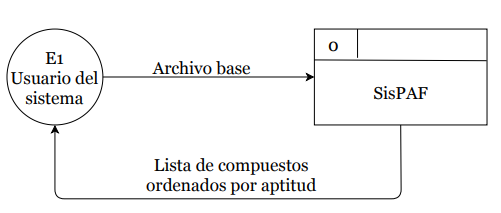
\includegraphics[scale=0.7]{Capitulo2/images/DFDContext.png}
    \caption{Nivel de contexto.}
    \label{nivel contexto}
\end{figure}
%%%%%%%
\begin{figure}[H]
    \centering
    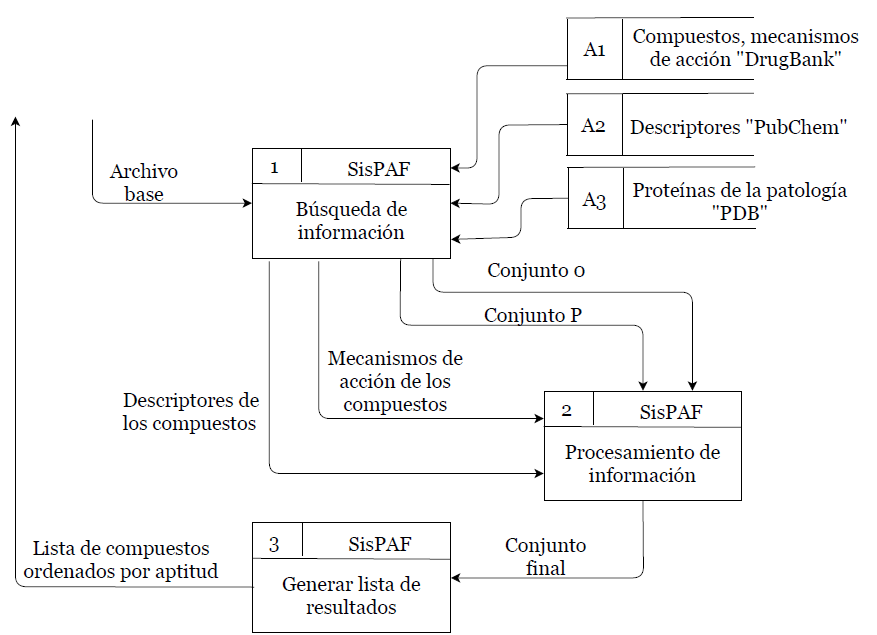
\includegraphics[scale=0.65]{Capitulo2/images/DFDN-1.png}
    \caption{Nivel 1}
    \label{nivel_1}
\end{figure}
%%%%%%%
\begin{figure}[H]
    \centering
    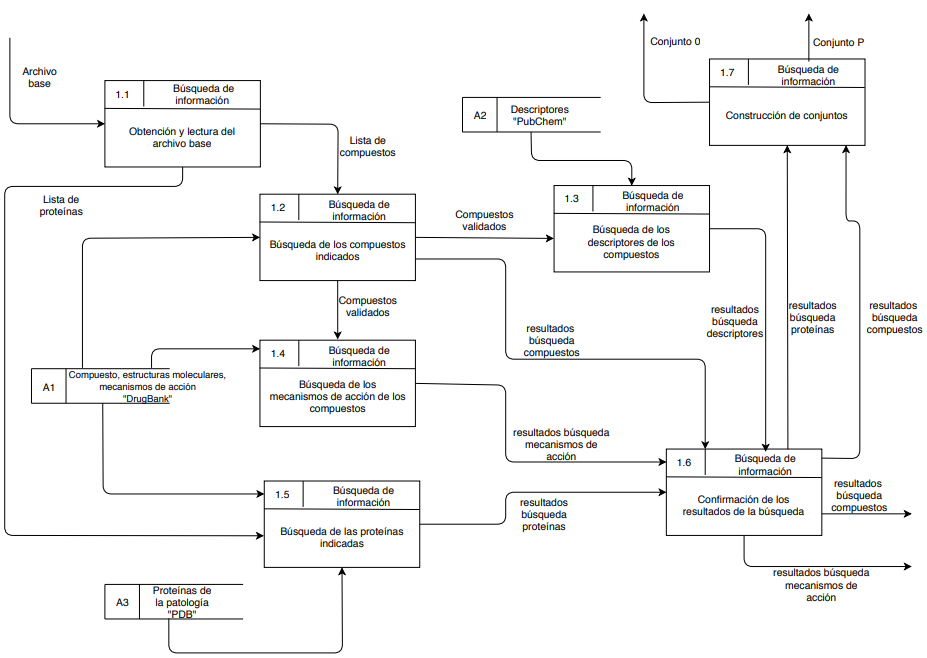
\includegraphics[scale=0.5]{Capitulo2/images/DFD-1.png}
    \caption{Nivel 2 - Requerimiento 1}
    \label{nivel_2_req1}
\end{figure}
%%%%%%%
\begin{figure}[H]
    \centering
    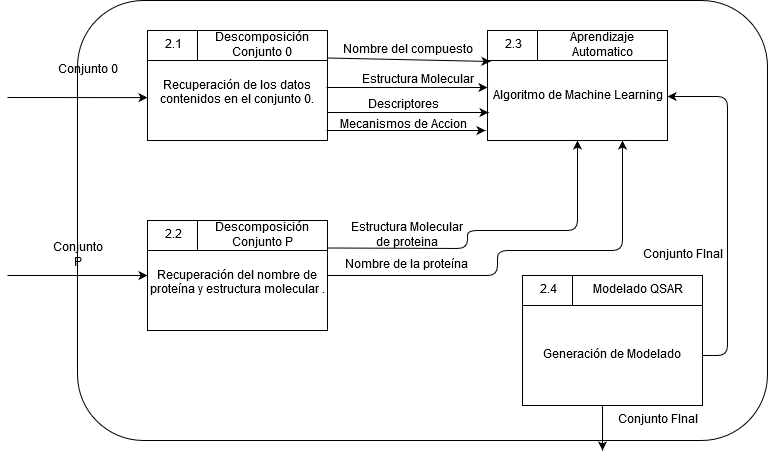
\includegraphics[scale=0.55]{Capitulo2/images/Req2.png}
    \caption{Nivel 2 - Requerimiento 2}
    \label{nivel_2_req2}
\end{figure}
%%%%%%%
\begin{figure}[H]
    \centering
    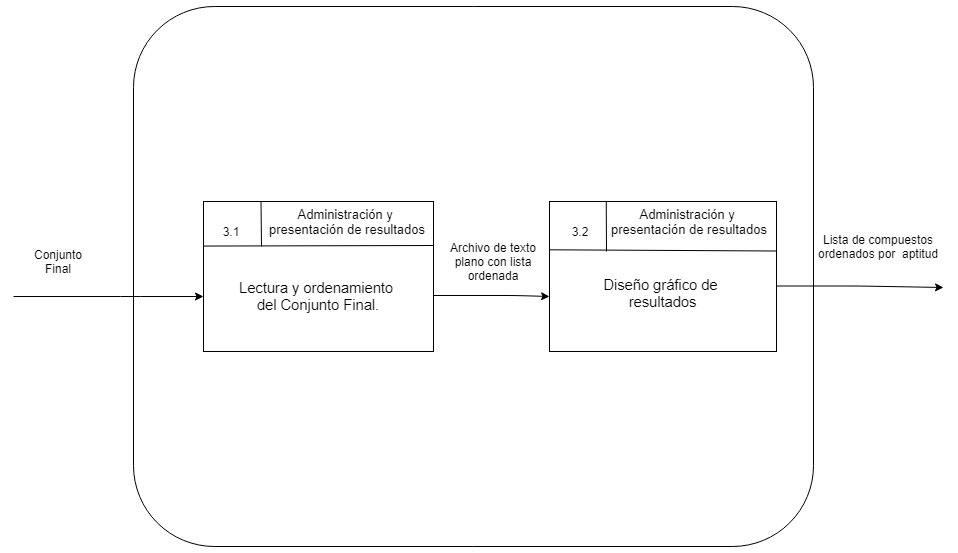
\includegraphics[scale=0.5]{Capitulo2/images/DFD-RF3.png}
    \caption{Nivel 2 - Requerimiento 3}
    \label{nivel_2_req3}
\end{figure}
%%%%%%%
%%%%%%%%%%%%%%%%%%%%%%%%%%%%%%%%%%%%%%%%%%%%%%%
\section{Modelo de Datos}
%%%%%%%%%
\begin{figure}[H]
    \centering
    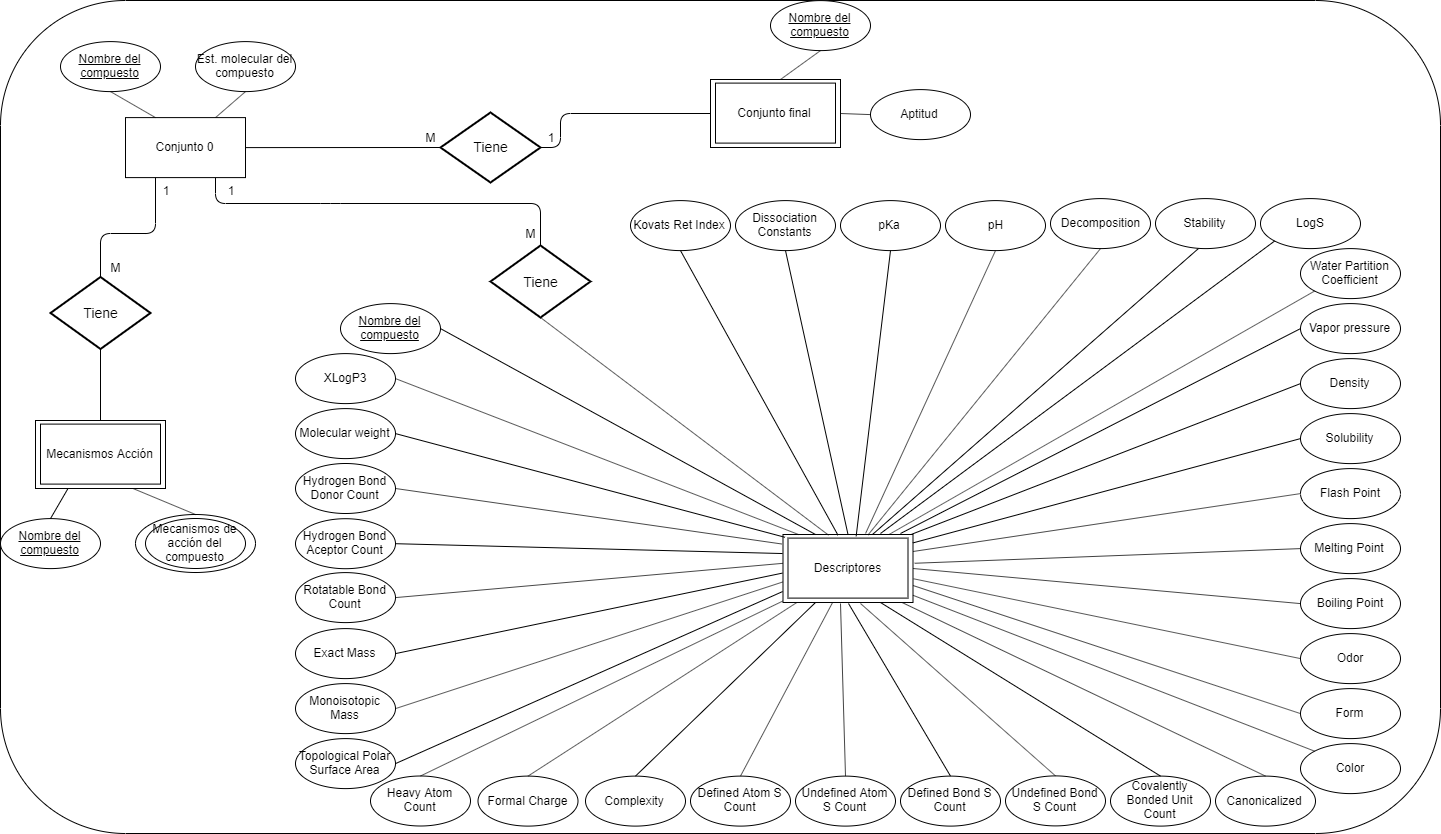
\includegraphics[scale=0.3]{Capitulo2/images/ModeloConceptualDatos.png}
    \caption{Modelo Conceptual de Datos}
    \label{modelo_conceptual}
\end{figure}
%%%%%%%%%
\begin{figure}[H]
    \centering
    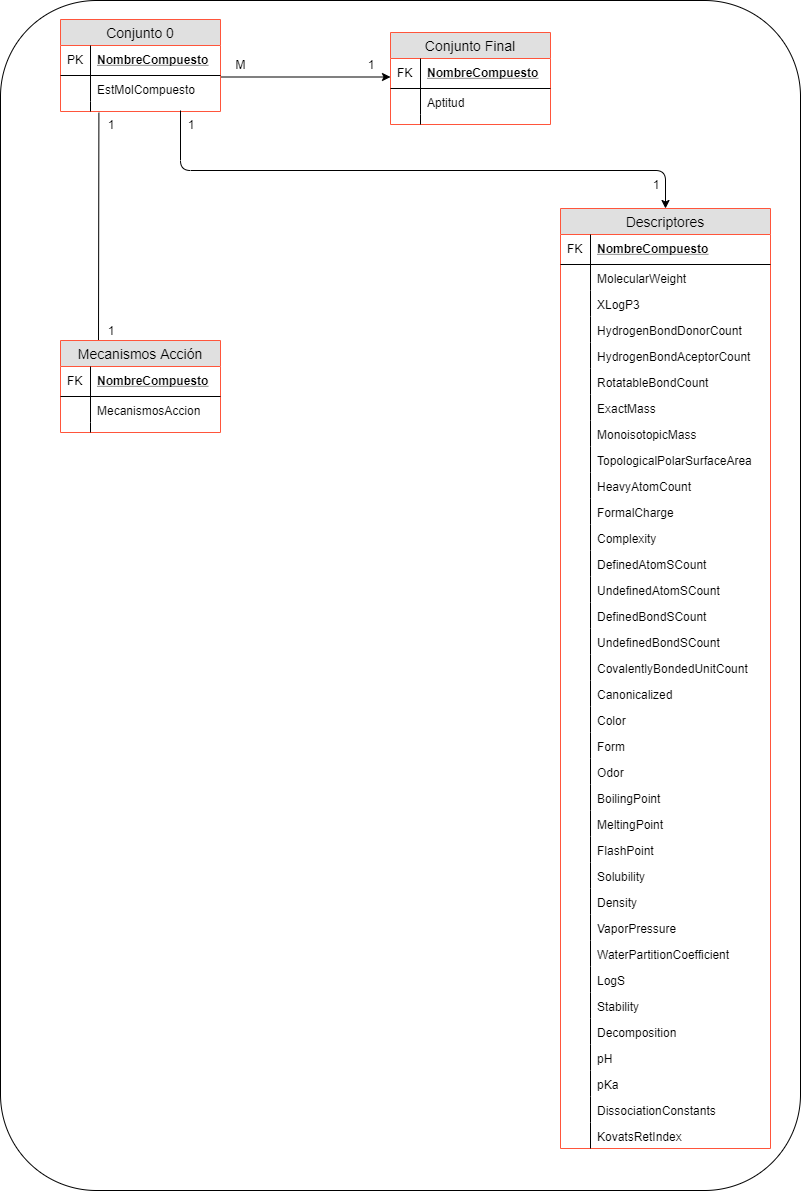
\includegraphics[scale=0.4]{Capitulo2/images/modeloDatosLogico.png}
    \caption{Modelo Lógico de Datos}
    \label{fig:my_label}
\end{figure}
%%%%%%%%
%%%%%%%%%%%%%%%%%%%%%%%%%%%%%%%%%%%%%%%%%%%%%%
\section{Interfaces de usuario} 
\noindent La metodología que pone la base en la cual se desarrolla este proyecto, indica una serie de puntos a tomar en cuenta cuando se realiza el prototipado (medio a través del cual se simula el aspecto visual del sistema mediante la representación de los conceptos, componentes, objetos gráficos, entradas y salidas requeridas para la ejecución de cada función en respuesta a las necesidades planteadas), con el fin de conseguir una interfaz eficiente y compatible con las necesidades de los usuarios. Los puntos se indican en la siguiente lista:\\

-	El principal punto que considerar y que constituye la base sobre la que se centra el diseño de prototipos es la identificación de los usuarios a los que va dirigido.\\

-	Analizar las funciones que va a soportar el sistema, con el fin de establecer las dependencias existentes entre ellas y su secuencia de ejecución.
-	Utilizar conceptos, términos y símbolos familiares al usuario, de modo que sea fácil de aprender y comprender.\\

-	Mantener la coherencia dentro del propio sistema y entre sistemas.\\

-	Facilitar la exploración del sistema sin riesgo, permitiendo interrumpir y deshacer las acciones realizadas. De esta forma, el usuario puede utilizar todas las funcionalidades del sistema y trabajar de forma más rápida y eficiente, con la seguridad de que cualquier error puede rectificarse.\\

-	Dificultar la selección de acciones destructivas y no reversibles, pidiéndole verificación de cualquier acción que conlleve un riesgo importante.\\

-	Proporcionar información sobre el estado de ejecución de las funciones, es decir, si la función invocada está en proceso, si se ha completado satisfactoriamente o se ha producido algún error.\\

-	Agrupar las funciones de forma lógica y presentar primero las más utilizadas.\\

-	Buscar la eficiencia en el diálogo evitando cambios frecuentes entre los dispositivos de entrada, tales como el ratón y el teclado.\\

\noindent Una vez tomados en cuenta esos puntos para realizar el diseño, para definir los formatos individuales de las pantallas se realiza un análisis de la información a presentar en cada una de ellas. Este análisis se debe centrar en los siguientes puntos:\\

-	Identificar los diferentes tipos de información como, por ejemplo, campos de datos, títulos, comandos y mensajes de error, con el fin de organizar la pantalla en áreas específicas y conseguir un equilibrio, regularidad, secuencialidad, así́ como, una simetría en la composición de las mismas.\\

-	Estudiar el espacio disponible en las pantallas para determinar qué datos y en qué situación deben aparecer en las mismas, utilizando un formato de visualización que permita al usuario una rápida asimilación de la información.\\

-	Intentar agrupar los datos relacionados y mostrar solo aquellos que son esenciales para la ejecución de la función o para la toma de una decisión, eliminado todas las entradas que sean innecesarias. Nunca se debe pedir al usuario que introduzca información que pueda adquirirse  automáticamente o calcularse internamente.\\

-	Mantener la coherencia entre la entrada y la visualización de datos.\\

-	Proteger al usuario de intentar alguna acción que podría provocar errores, desactivando los comandos que no son operativos en ese contexto.\\

\noindent Todo esto es tomado en cuenta para el prototipado de interfaces y para su futuro desarrollo e implementación en el código.\\

\noindent En esta actividad se especifican las interfaces entre el sistema y el usuario: formatos de
pantallas, diálogos, e informes, principalmente. El objetivo es realizar un análisis de los
procesos del sistema de información en los que se requiere una interacción del usuario, con el
fin de crear una interfaz que satisfaga todos los requisitos establecidos, teniendo en cuenta los
diferentes perfiles a quiénes va dirigido.\\

\noindent Para el desarrollo de interfaces nos basaremos en la ISO 9241 (Proceso de Diseño Centrado en Usuarios) la cual nos proporciona una guía de actividades a través del ciclo de vida de los sistemas interactivos, que consisten en cuatro tipos diferentes de actividades.\\

\noindent• Entender y especificar el contexto de uso.\\
• Especificar los requerimientos de la organización y del usuario.\\
• Proceder a diseñar soluciones.\\
• Evaluar los diseños con respecto a los requerimientos.\\
De las cuales nos enfocaremos en las últimas dos etapas donde se desarrollarán las siguientes actividades:\\

\noindent 1.Realizaremos diseños de prototipos de nuestro producto con el fin de que pueda ser evaluado.\\
2.Se representará cómo los usuarios pueden interactuar con la aplicación o proyecto.\\
3.Crear un plan de evaluación.\\
4.Reportar los resultados de la evaluación y las recomendaciones de cambio.\\
4.1.Iterar esta actividad hasta que el objetivo del diseño sean logrados.\\
Para poder realizar la actividad 3, debemos crear un plan de evaluación, por lo cual nosotros decidimos tomar un plan creado para evaluar interfaces de windows llamada “Windows: GUI Guidelines 4.1” creada por la empresa “ADD Servicios Informáticos S.A”.\\

\noindent Estas recomendaciones fueron implementadas para un proyecto en específico llamado “Proyecto BOE”, por lo cual se hicieron adecuaciones con respecto a nuestro sistema.\\

 \noindent Estos estándares se encuentran definidos y evaluados en la tabla \ref{estandares}, donde se encuentra definida la norma, su tarea y el como aplica en nuestro proyecto.\\

\subsection{Pantallas del sistema}
\noindent Las siguientes pantallas del sistema muestran los procesos mas importantes con las cuales el usuario tendrá que interactuar.
%%%%%%%%%%%%%%%%%%%%%%%%%%%%%%%%%
\begin{figure}[H]
    \centering
    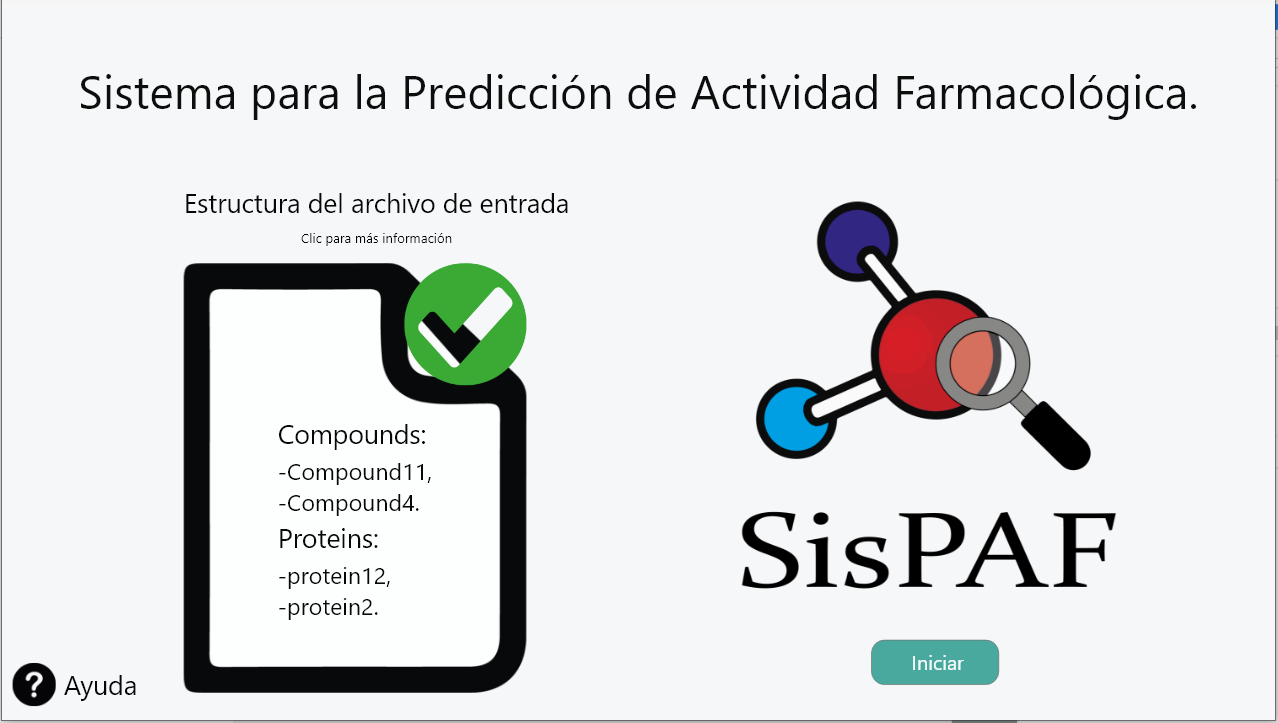
\includegraphics[scale=0.4]{Capitulo2/images/UI/1_tutorial.PNG}
    \caption{Tutorial del archivo base}
    \label{Tutorial_1}
\end{figure}
%%%%%%%%%%%%%%%%%%%%%%%%%%%%%%%
\begin{figure}[H]
    \centering
    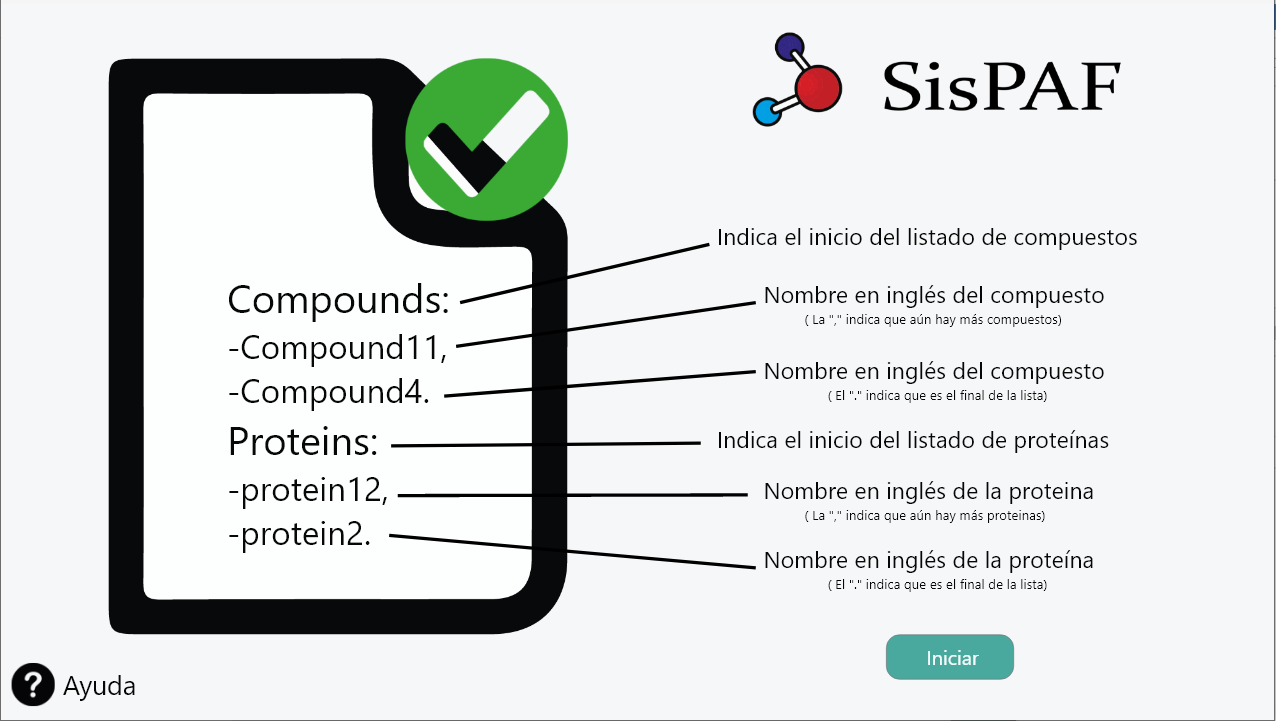
\includegraphics[scale=0.4]{Capitulo2/images/UI/2_tutorial.PNG}
    \caption{Especificación de la estructural del archivo base }
    \label{Tutorial_2}
\end{figure}
%%%%%%%%%%%%%%%%%%%%%%%%%%%%%%
\begin{figure}[H]
    \centering
    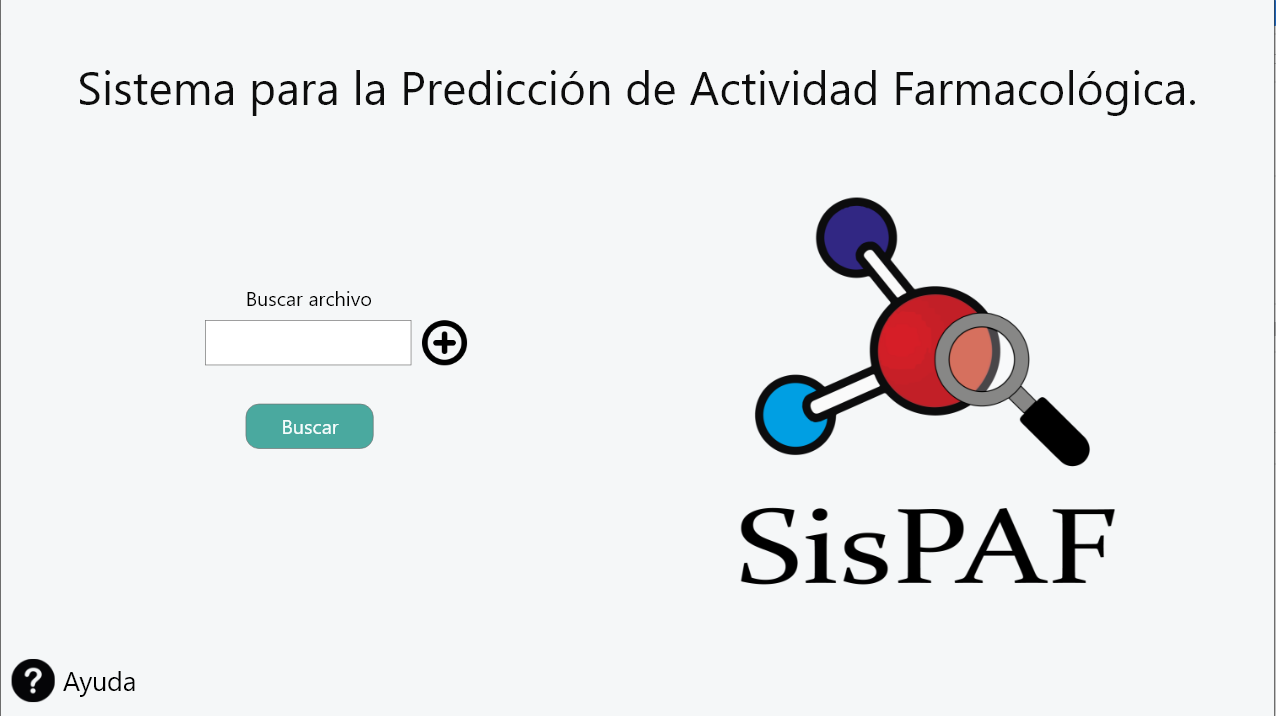
\includegraphics[scale=0.4]{Capitulo2/images/UI/3_pantalla_inicio.PNG}
    \caption{Pantalla de inicio}
    \label{Pantalla_de_inicio}
\end{figure}
%%%%%%%%%%%%%%%%%%%%%%%%%%%%%
\begin{figure}[H]
    \centering
    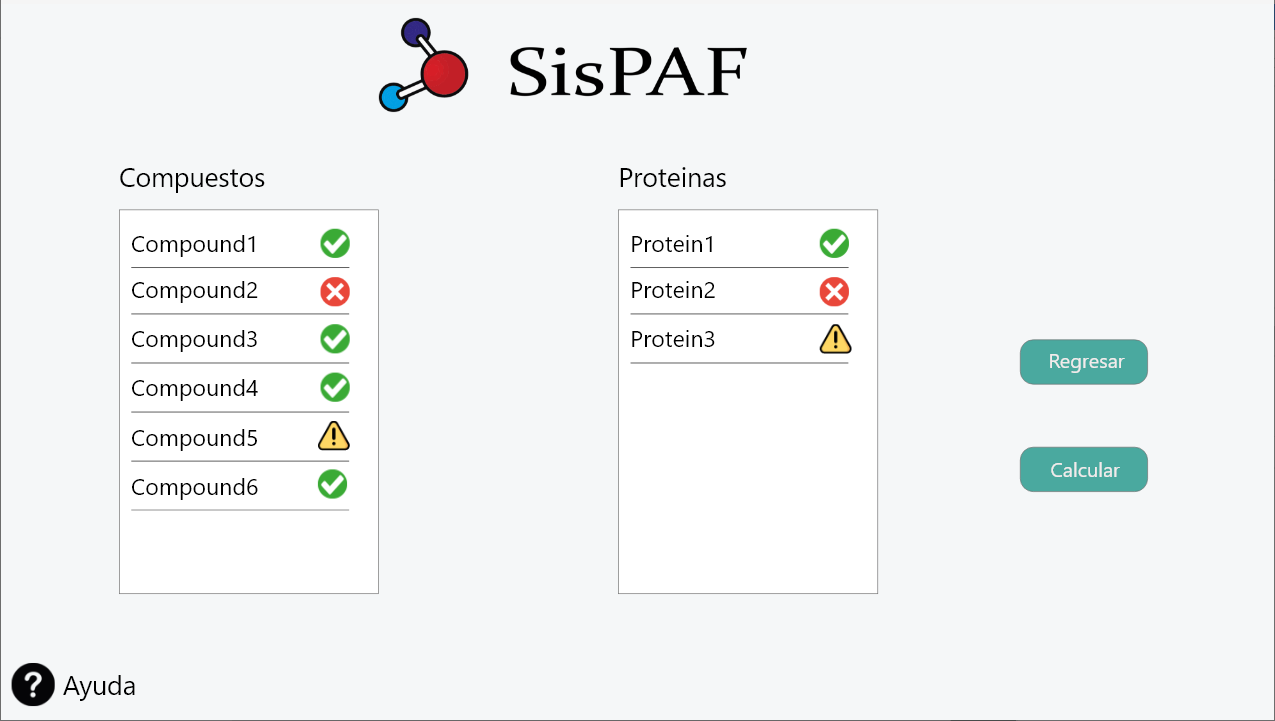
\includegraphics[scale=0.4]{Capitulo2/images/UI/5_preeliminar.PNG}
    \caption{Pantalla preliminar de los elementos encontrados}
    \label{preliminar}
\end{figure}
%%%%%%%%%%%%%%%%%%%%%%%%%%%%%
\begin{figure}[H]
    \centering
    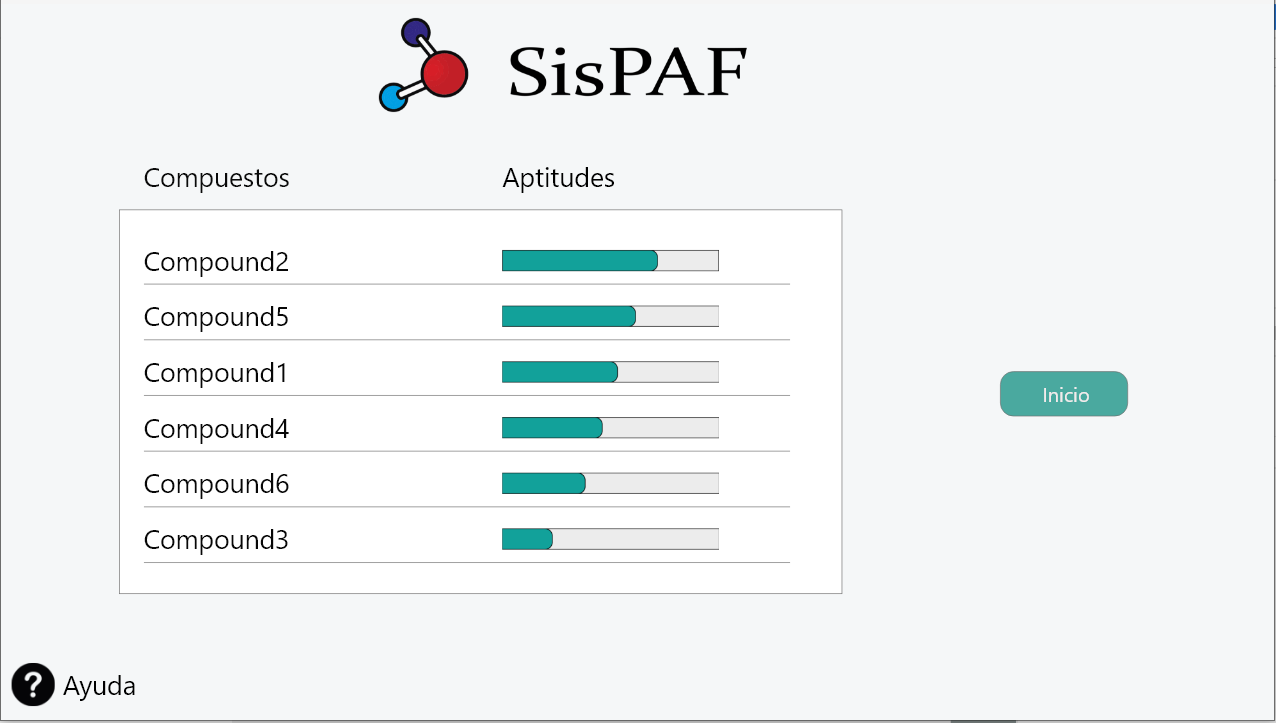
\includegraphics[scale=0.4]{Capitulo2/images/UI/7_resultados.PNG}
    \caption{Resultado arrojado por el sistema (Lista ordenada)}
    \label{Resultados}
\end{figure}
%%%%%%%%%%%%%%%%%%%%%%%%%%%%%
\subsubsection{Pantallas secundarias}
\noindent En este apartado se muestran las pantallas secundarias del sistemas, en la cual solo es cuestión del termino de un proceso interno del sistema. Por lo cual no necesita mayor interacción del usuario.
%%%%%%%%%%%%%%5
\begin{figure}[H]
    \centering
    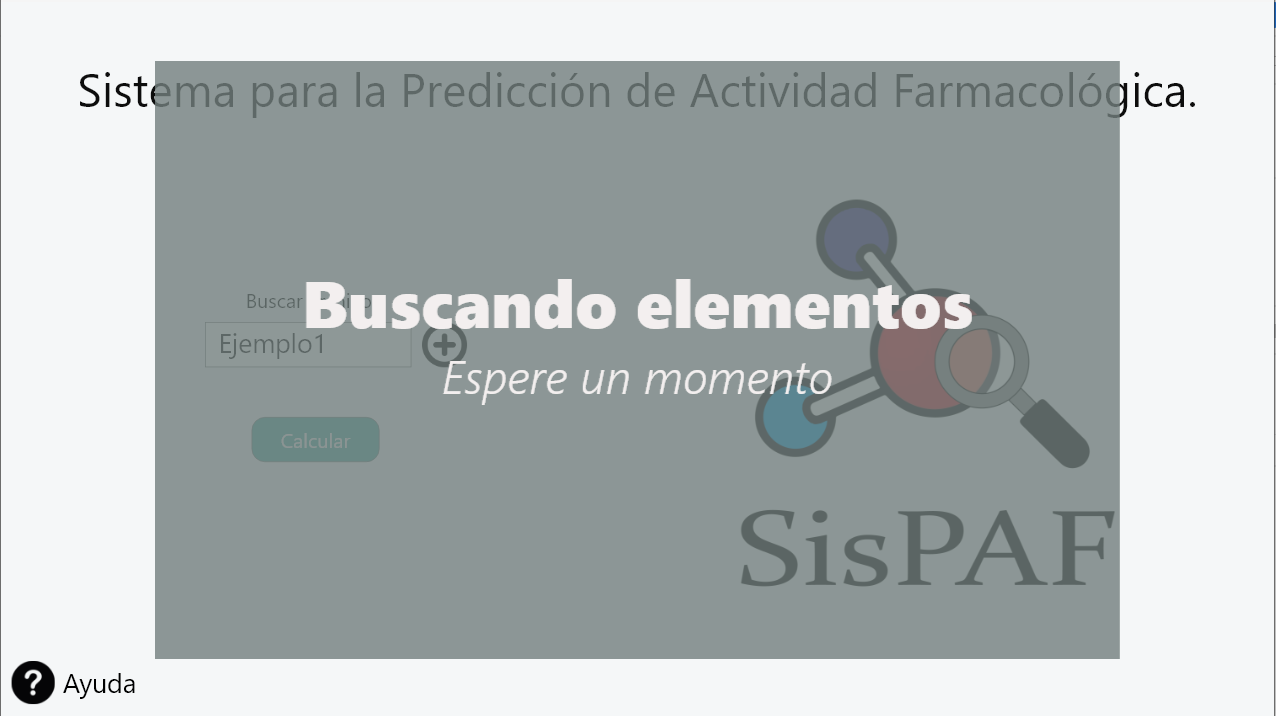
\includegraphics[scale=0.4]{Capitulo2/images/UI/4_Espera_busqueda.PNG}
    \caption{Pantalla de espera mientras la búsqueda de datos se ejecuta}
    \label{Espera_busq}
\end{figure}
%%%%%%%%%%%%%%
\begin{figure}[H]
    \centering
    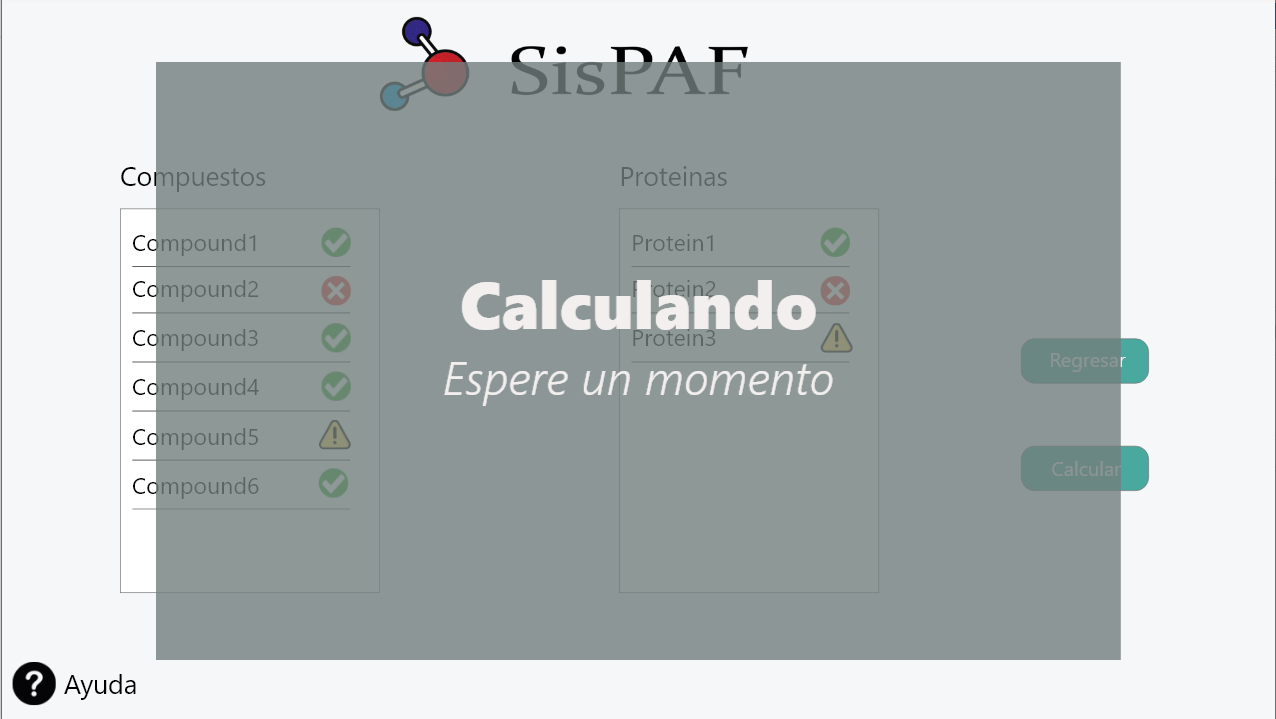
\includegraphics[scale=0.4]{Capitulo2/images/UI/6_espera_calculo.PNG}
    \caption{Pantalla de espera mientras e calculo se efectúa}
    \label{Espera_cal}
\end{figure}
%%%%%%%%%%%%%%%
\subsubsection{Mensajes}
\noindent Estos son los mensajes que se pueden mostrar al usuario por una posible excepción del sistema. 
\begin{figure}[H]
    \centering
    
\includegraphics[scale=0.4]{Capitulo2/images/UI/9_error_conexion.PNG}
    \caption{Mensaje de error de conexión}
    \label{Mensaje_error}
\end{figure}
%%%%%%%%%%%%%%%
\begin{figure}[H]
    \centering
    
\includegraphics[scale=0.4]{Capitulo2/images/UI/10_error_archivo.PNG}
    \caption{Mensaje de error de archivo}
    \label{error_de_Arch}
\end{figure}
%%%%%%%%%%%%%%%%
\begin{figure}[H]
    \centering
    
\includegraphics[scale=0.4]{Capitulo2/images/UI/11_error_datos.PNG}
    \caption{Mensaje de error de datos}
    \label{error_de_datos_notf}
\end{figure}
%%%%%%%%%%%%%%%%
\begin{figure}[H]
    \centering
    
\includegraphics[scale=0.4]{Capitulo2/images/UI/13_advertencia.PNG}
    \caption{Advertencia de datos incompletos}
    \label{advertencia}
\end{figure}

%%%%%%%%%%%%%%%%%%%%%%%%%%%%%%%%%%%%55
\section{Plan de acción}

%Plan de pruebas unitarias
\subsection{Pruebas Unitarias}
\noindent \textbf{Definición:} Verificar la funcionalidad y estructura de cada componente de manera individual.\\
\textbf{Enfoque a usar:} Funcional-Caja negra.\\
\textbf{Descripción:} Se comprueba el correcto funcionamiento de los componentes del sistema de información, analizando las entradas y salidas y verificando que el resultado es el esperado. Se consideran exclusivamente las entradas y salidas del sistema sin preocuparse por la estructura interna del mismo.\\
%%%%%%%%%%%%%%%%%%%%
% Please add the following required packages to your document preamble:
% \usepackage{longtable}
% Note: It may be necessary to compile the document several times to get a multi-page table to line up properly
\begin{longtable}{|l|l|}
\caption{Prueba unitaria RF1.1}
\label{PU_RF1_1}\\
\hline

\textbf{Requerimiento Funcional}                                                       & \textbf{RF1.1 Adquisición del archivo base.}                                                                                                                                                                                                                                                                                                                                                                                                                                                                                                                                                                                                                                                     \\ \hline
\endfirsthead
%
\multicolumn{2}{c}%
{{\bfseries Tabla \thetable\ Continuación de la página anterior}} \\
\endhead
%
\textbf{Perfiles Implicados}                                                           & \begin{tabular}[c]{@{}l@{}}- Desarrollador.\\ - Tester.\end{tabular}                                                                                                                                                                                                                                                                                                                                                                                                                                                                                                                                                                                                                             \\ \hline
\textbf{Planificación temporal}                                                        & \begin{tabular}[c]{@{}l@{}}1. Prueba de compilación.\\ 2. Prueba de funcionamiento.\\ 2.1 Func. botón adquisición archivo.\\ 2.2 Muestra de pantalla selección de\\ archivo.\\ 2.3 Acceso a directorio.\\ 2.4 Carga de archivo.\\ 2.5 Func. botón buscar.\end{tabular}                                                                                                                                                                                                                                                                                                                                                                                                                           \\ \hline
\textbf{Criterio de verificación}                                                      & \begin{tabular}[c]{@{}l@{}}1. Compilación del código.\\ 2. Ejecutable del módulo, hay muestras\\ de que el código hace algo (algo: definido por los \\ siguientes puntos).\\ 2.1 Funcionamiento del botón de Archivo base.\\ 2.2 Visualización de selección de archivo.\\ 2.3 Acceso al directorio correcto o permite acceder \\ a uno distinto desde la pantalla de selección de \\ archivo.\\ 2.4 Carga del archivo correcto.\\ 2.5 El botón se ve adecuadamente y accede al\\ archivo indicado y logra una lectura correcta.\end{tabular}                                                                                                                                                     \\ \hline
\textbf{Criterio de aceptación}                                                        & \begin{tabular}[c]{@{}l@{}}1. No hay errores que impidan la compilación \\ del código.\\ 2. Al usar el ejecutable del módulo, hay muestras \\ de que el código hace algo \\ (algo: definido por los siguientes puntos).\\ 2.1 Se muestra el botón correspondiente, y realiza la \\ acción indicada.\\ 2.2 Es visualizada la pantalla de selección de archivos \\ con cada uno de los componentes.\\ 2.3 La selección de archivos se encuentra en el \\ directorio correcto o permite acceder a uno distinto.\\ 2.4 Solo permite la carga de un archivo de texto \\ plano, y es cargado adecuadamente.\\ 2.5 El botón se ve adecuada, y realiza la acción \\ indicada correctamente.\end{tabular} \\ \hline
\textbf{\begin{tabular}[c]{@{}l@{}}Definición de\\ verificaciones\end{tabular}}        & \begin{tabular}[c]{@{}l@{}}- Errores de Compilación: Ocurren porque la sintaxis \\ del lenguaje no es correcta, de cajón este tipo de \\ errores no permiten que la aplicación se ejecute. \\ \\ - Acción de botón: representa un botón que, cuando \\ es presionado, envía información al que pertenece. \\ La función de  un botón representada  el contenido\\ del elemento.\\ \\ -Visualización de pantalla interfaz de usuario.\end{tabular}                                                                                                                                                                                                                                                \\ \hline
\textbf{\begin{tabular}[c]{@{}l@{}}Análisis y evaluación\\ de resultados\end{tabular}} &                                                                                                                                                                                                                                                                                                                                                                                                                                                                                                                                                                                                                                                                                                  \\ \hline
\textbf{Productos  a entregar}                                                         & \begin{tabular}[c]{@{}l@{}}- Adquisición del archivo base funcionando \\ correctamente.\end{tabular}                                                                                                                                                                                                                                                                                                                                                                                                                                                                                                                                                                                             \\ \hline

\end{longtable}
% Please add the following required packages to your document preamble:
% \usepackage{longtable}
% Note: It may be necessary to compile the document several times to get a multi-page table to line up properly
\begin{longtable}{|l|l|}
\caption{Caso de prueba RF1}
\label{CP_RF1}\\
\hline
\textbf{ID del Caso de prueba}                                                          & CPRF1                                                                                                                                                            \\ \hline
\endfirsthead
%
\multicolumn{2}{c}%
{{\bfseries Tabla \thetable\ Continuación de la página anterior}} \\
\endhead
%
\textbf{Versión}                                                                        & 1.0                                                                                                                                                              \\ \hline
\textbf{Nombre}                                                                         & Caso de prueba para adquisición de archivo base.                                                                                                                 \\ \hline
\textbf{\begin{tabular}[c]{@{}l@{}}Identificador de \\ requerimiento\end{tabular}}      & RF1.1                                                                                                                                                            \\ \hline
\textbf{Propósito}                                                                      & \begin{tabular}[c]{@{}l@{}}Determinar capacidad del sistema para \\ obtener el archivo base.\end{tabular}                                                        \\ \hline
\textbf{Dependencias}                                                                   & N/A                                                                                                                                                              \\ \hline
\textbf{\begin{tabular}[c]{@{}l@{}}Ambiente de \\ prueba/configuración\end{tabular}}    & \begin{tabular}[c]{@{}l@{}}- Hardware: Equipo de computo\\ (preferentemente portatíl)\\ - Software: Compilador python3, \\ IDE y/o editor de texto.\end{tabular} \\ \hline
\textbf{Inicialización}                                                                 & \begin{tabular}[c]{@{}l@{}}- Codificación correspondiente al \\ requerimiento.\\ - Creación del archivo base.\end{tabular}                                       \\ \hline
\textbf{Finalización}                                                                   & N/A                                                                                                                                                              \\ \hline
\textbf{Acciones}                                                                       & \begin{tabular}[c]{@{}l@{}}. Compilar el código correspondiente.\\ - Colocar el archivo en el directorio \\ especificado.\end{tabular}                           \\ \hline
\textbf{\begin{tabular}[c]{@{}l@{}}Descripción de los \\ datos de entrada\end{tabular}} & \begin{tabular}[c]{@{}l@{}}- Archivo de texto plano.\\ - Directorio de la ubicación del archivo base.\end{tabular}                                               \\ \hline
\textbf{Salida esperada}                                                                & \begin{tabular}[c]{@{}l@{}}- Notificación de adecuada adquisición del \\ archivo base.\end{tabular}                                                              \\ \hline
\textbf{Salida obtenida}                                                                &                                                                                                                                                                  \\ \hline
\textbf{Resultado}                                                                      &                                                                                                                                                                  \\ \hline
\textbf{Severidad}                                                                      &                                                                                                                                                                  \\ \hline
\textbf{Evidencia}                                                                      &                                                                                                                                                                  \\ \hline
\textbf{Estado}                                                                         & No Iniciado.                                                                                                                                                     \\ \hline
\end{longtable}

%%%%%%%%%%%%%%%%%%%%
% Please add the following required packages to your document preamble:
% \usepackage{longtable}
% Note: It may be necessary to compile the document several times to get a multi-page table to line up properly
\begin{longtable}{|l|l|}
\caption{Prueba unitaria RF1.2}
\label{PU_RF1_2}\\
\hline
\textbf{Requerimiento Funcional}                                                       & \textbf{RF1.2 Búsqueda de los compuestos indicados..}                                                                                                                                                                                                                                                                                                                                                                                                                                                                                                                                  \\ \hline
\endfirsthead
%
\multicolumn{2}{c}%
{{\bfseries Table \thetable\ Continuación de la página anterior}} \\
\endhead
%
\textbf{Perfiles Implicados}                                                           & \begin{tabular}[c]{@{}l@{}}- Desarrollador.\\ - Tester.\end{tabular}                                                                                                                                                                                                                                                                                                                                                                                                                                                                                                                   \\ \hline
\textbf{Planificación temporal}                                                        & \begin{tabular}[c]{@{}l@{}}1. Prueba de compilación.\\ 2. Prueba de funcionamiento.\\ 2.1 Verificar adecuada lectura del archivo base\\ (token “compunds” ).\\ 2.2 Comprobar conexión a la base de datos \\ “DrugBank”.\\ 2.3 Obtención del .pdb de cada uno de los \\ compuestos enlistados.\\ 2.4 Almacenado del .pdb en el sistema.\end{tabular}                                                                                                                                                                                                                                   \\ \hline
\textbf{Criterio de verificación}                                                      & \begin{tabular}[c]{@{}l@{}}1. Compilación del código.\\ 2. Ejecutable del módulo, hay muestras de que el \\ código hace algo\\ (algo: definido por los siguientes puntos).\\ 2.1 Lectura del token que describe los nombres del\\ compuesto en el archivo base.\\ 2.2 Conexión a  DrugBank y por lo tanto a Internet.\\ 2.3 Adquirir el archivo .pdb del compuesto correcto.\\ 2.4 Almacenamiento de un archivo íntegro en el \\ sistema.\end{tabular}                                                                                                                                \\ \hline
\textbf{Criterio de aceptación}                                                        & \begin{tabular}[c]{@{}l@{}}1. No hay errores que impidan la compilación del \\ código.\\ 2. Al usar el ejecutable del módulo, hay muestras \\ de que el código hace algo\\ (algo: definido por los siguientes puntos).\\ 2.1 No se pierde ningún valor ni dato existente en el\\ archivo base.\\ 2.2 El sistema informa la correcta conexión a \\ “DrugBank”.\\ 2.3 El sistema informa que el compuesto existe \\ en la base de datos y confirma la adquisición \\ del .pdb.\\ 2.4 El sistema notifica la correcta obtención del \\ archivo .pdb y correcto  almacenado.\end{tabular} \\ \hline
\textbf{\begin{tabular}[c]{@{}l@{}}Definición de\\ verificaciones\end{tabular}}        & \begin{tabular}[c]{@{}l@{}}- Errores de Compilación: Ocurren porque la sintaxis \\ del lenguaje no es correcta, de cajón este tipo de \\ errores no permiten que la aplicación se ejecute. \\ \\ - Conexión a base de datos online:Una conexión a \\ base de datos es un archivo de configuración donde \\ se especifica los detalles físicos de una base de datos \\ como por ejemplo el tipo de base de datos y la \\ versión, y los parámetros que permiten una conexión\end{tabular}                                                                                               \\ \hline
\textbf{\begin{tabular}[c]{@{}l@{}}Análisis y evaluación\\ de resultados\end{tabular}} &                                                                                                                                                                                                                                                                                                                                                                                                                                                                                                                                                                                        \\ \hline
\textbf{Productos  a entregar}                                                         & \begin{tabular}[c]{@{}l@{}}- Búsqueda de los compuestos indicados \\ funcionando correctamente.\end{tabular}                                                                                                                                                                                                                                                                                                                                                                                                                                                                           \\ \hline
\end{longtable}
% Please add the following required packages to your document preamble:
% \usepackage{longtable}
% Note: It may be necessary to compile the document several times to get a multi-page table to line up properly
\begin{longtable}{|l|l|}
\caption{Caso de prueba RF1.2}
\label{CP_RF1_2}\\
\hline
\textbf{ID del Caso de prueba}                                                          & CPRF2                                                                                                                                                                                                                                        \\ \hline
\endfirsthead
%
\multicolumn{2}{c}%
{{\bfseries Tabla \thetable\ Continuación de la página anterior}} \\
\endhead
%
\textbf{Versión}                                                                        & 1.0                                                                                                                                                                                                                                          \\ \hline
\textbf{Nombre}                                                                         & \begin{tabular}[c]{@{}l@{}}Caso de prueba para la búsqueda de los \\ compuestos indicados.\end{tabular}                                                                                                                                      \\ \hline
\textbf{\begin{tabular}[c]{@{}l@{}}Identificador de \\ requerimiento\end{tabular}}      & RF1.2                                                                                                                                                                                                                                        \\ \hline
\textbf{Propósito}                                                                      & \begin{tabular}[c]{@{}l@{}}Calificar la búsqueda del compuesto en la base \\ de datos “Drug Bank” , desde obtener el nombre \\ en el archivo base a la adquisición del .pdb.\end{tabular}                                                  \\ \hline
\textbf{Dependencias}                                                                   & Correcta obtención del archivo base.                                                                                                                                                                                                         \\ \hline
\textbf{\begin{tabular}[c]{@{}l@{}}Ambiente de \\ prueba/configuración\end{tabular}}    & \begin{tabular}[c]{@{}l@{}}- Hardware: Equipo de computo\\ (preferentemente portatíl)\\ - Software: Compilador python3, \\ IDE y/o editor de texto.\end{tabular}                                                                             \\ \hline
\textbf{Inicialización}                                                                 & \begin{tabular}[c]{@{}l@{}}- Codificación correspondiente al \\ requerimiento.\\ - Creación del archivo base.\end{tabular}                                                                                                                   \\ \hline
\textbf{Finalización}                                                                   & N/A                                                                                                                                                                                                                                          \\ \hline
\textbf{Acciones}                                                                       & \begin{tabular}[c]{@{}l@{}}. Compilar el código correspondiente.\\ - Contar con el archivo base previamente \\ cargado.\end{tabular}                                                                                                         \\ \hline
\textbf{\begin{tabular}[c]{@{}l@{}}Descripción de los \\ datos de entrada\end{tabular}} & \begin{tabular}[c]{@{}l@{}}- Archivo de texto plano.\\ - Dirección para la conexión a “Drug Bank”.\end{tabular}                                                                                                                              \\ \hline
\textbf{Salida esperada}                                                                & \begin{tabular}[c]{@{}l@{}}Notificación de adecuada estado del \\ compuesto en “Drug Bank” (Existente o no).\\ - De existir, informar que el compuesto \\ existe al igual que el archivo .pdb\\ - Adquisición correcta del .pdb\end{tabular} \\ \hline
\textbf{Salida obtenida}                                                                &                                                                                                                                                                                                                                              \\ \hline
\textbf{Resultado}                                                                      &                                                                                                                                                                                                                                              \\ \hline
\textbf{Severidad}                                                                      &                                                                                                                                                                                                                                              \\ \hline
\textbf{Evidencia}                                                                      &                                                                                                                                                                                                                                              \\ \hline
\textbf{Estado}                                                                         & No Iniciado.                                                                                                                                                                                                                                 \\ \hline
\end{longtable}

%%%%%%%%%%%%%%%%%%%%
% Please add the following required packages to your document preamble:
% \usepackage{longtable}
% Note: It may be necessary to compile the document several times to get a multi-page table to line up properly
\begin{longtable}{|l|l|}
\caption{Prueba unitaria RF1.3}
\label{PU_RF1_3}\\
\hline
\textbf{Requerimiento Funcional}                                                       & \textbf{\begin{tabular}[c]{@{}l@{}}RF1.3 Búsqueda de los descriptores de los \\ compuestos.\end{tabular}}                                                                                                                                                                                                                                                                                                                                                                                                                                                                                                                                                                                                                                                                                                                                                                                      \\ \hline
\endfirsthead
%
\multicolumn{2}{c}%
{{\bfseries Tabla \thetable\ Continuación de la página anterior}} \\
\endhead
%
\textbf{Perfiles Implicados}                                                           & \begin{tabular}[c]{@{}l@{}}- Desarrollador.\\ - Tester.\end{tabular}                                                                                                                                                                                                                                                                                                                                                                                                                                                                                                                                                                                                                                                                                                                                                                                                                           \\ \hline
\textbf{Planificación temporal}                                                        & \begin{tabular}[c]{@{}l@{}}1. Prueba de compilación.\\ 2. Prueba de funcionamiento.\\ 2.1 Verificar que el sistema mantiene el nombre \\ del compuesto sobre del que están obteniendo \\ los datos.\\ 2.2 Comprobar conexión a la base de datos \\ “ChemSpider” y “PubChem”.\\ 2.3 Búsqueda del compuesto en las bases de \\ datos.\\ 2.3.1  Existe el compuesto con el nombre \\ exacto en “PubChem”. \\ 2.3.2 Existe el compuesto con el nombre \\ exacto en “ChemSpider”.\\ 2.4 Adquisición de los descriptores del \\ compuesto en las bases de datos.\\ 2.3.1  Se adquieren  los descriptores  existentes en \\ “PubChem” del compuesto. \\ 2.3.2 Se adquieren  los descriptores  existentes en \\ “ChemSpider” del compuesto.\\ 2.4 Creación del archivo “Descriptors”.\\ 2.5 Almacenado de los datos adquiridos en \\ el archivo correspondiente , recientemente creado.\end{tabular} \\ \hline
\textbf{Criterio de verificación}                                                      & \begin{tabular}[c]{@{}l@{}}1. Compilación del código.\\ 2. Ejecutable del módulo, hay muestras de que el \\ código hace algo\\ (algo: definido por los siguientes puntos).\\ 2.1Verificación de integridad de la variable que \\ contiene el nombre del compuesto.\\ 2.2 Conexión a  “ChemSpider” y “PubChem” \\ y por lo tanto a Internet.\\ 2.3 Adecuada búsqueda del del compuesto exacto \\ en la base de datos.\\ 2.3.1 Correcta adquisición de los descriptores en\\ “PubChem”.\\ 2.3.2 Correcta adquisición de los descriptores en\\ “ChemSpider”.\\ 2.4 Creación del archivo “Descriptors” \\ correspondiente con el compuesto.\\ 2.5 Corroborar guardado de la información \\ obtenida en el archivo creado.\end{tabular}                                                                                                                                                          \\ \hline
\textbf{Criterio de aceptación}                                                        & \begin{tabular}[c]{@{}l@{}}1. No hay errores que impidan la compilación \\ del código.\\ 2. Al usar el ejecutable del módulo, hay muestras \\ de que el código hace algo\\ (algo: definido por los siguientes puntos).\\ 2.1 No se distorsiona el nombre del compuesto \\ de interés.\\ 2.2 El sistema informa la correcta conexión a\\ “ChemSpider”.\\ 2.3 El sistema informa la correcta conexión a \\ “PubChem”.\\ 2.4 El sistema informa que el mismo compuesto \\ existe en ambos repositorios.\\ 2.5. Se notifica la adecuada obtención de los \\ descriptores del compuesto.\\ 2.6 El sistema informa la correcta creación del\\  archivo.\\ 2.7 El archivo y la información que contiene es \\ integra.\end{tabular}                                                                                                                                                                   \\ \hline
\textbf{\begin{tabular}[c]{@{}l@{}}Definición de\\ verificaciones\end{tabular}}        & \begin{tabular}[c]{@{}l@{}}- Errores de Compilación: Ocurren porque la \\ sintaxis del lenguaje no es correcta, de cajón \\ este tipo de errores no permiten que la \\ aplicación se ejecute. \\ \\ - Conexión a base de datos online: \\ Una conexión a base de datos es un archivo \\ de configuración donde se especifica los \\ detalles físicos de una base de datos como por \\ ejemplo el tipo de base de datos y la versión, y \\ los parámetros que permiten una conexión\end{tabular}                                                                                                                                                                                                                                                                                                                                                                                                \\ \hline
\textbf{\begin{tabular}[c]{@{}l@{}}Análisis y evaluación\\ de resultados\end{tabular}} & - Resultados:                                                                                                                                                                                                                                                                                                                                                                                                                                                                                                                                                                                                                                                                                                                                                                                                                                                                                  \\ \hline
\textbf{Productos  a entregar}                                                         & \begin{tabular}[c]{@{}l@{}}- Búsqueda de los descriptores correspondientes\\  al compuesto de interés.\end{tabular}                                                                                                                                                                                                                                                                                                                                                                                                                                                                                                                                                                                                                                                                                                                                                                            \\ \hline
\end{longtable}
% Please add the following required packages to your document preamble:
% \usepackage{longtable}
% Note: It may be necessary to compile the document several times to get a multi-page table to line up properly
\begin{longtable}{|l|l|}
\caption{Caso de prueba RF1.3}
\label{CP_RF1_3}\\
\hline
\textbf{ID del Caso de prueba}                                                          & CPRF3                                                                                                                                                                                                                                                          \\ \hline
\endfirsthead
%
\multicolumn{2}{c}%
{{\bfseries Tabla \thetable\ Continuación de la página anterior}} \\
\endhead
%
\textbf{Versión}                                                                        & 1.0                                                                                                                                                                                                                                                            \\ \hline
\textbf{Nombre}                                                                         & \begin{tabular}[c]{@{}l@{}}Caso de prueba para la búsqueda de los \\ descriptores de los compuestos.\end{tabular}                                                                                                                                              \\ \hline
\textbf{\begin{tabular}[c]{@{}l@{}}Identificador de \\ requerimiento\end{tabular}}      & RF1.3                                                                                                                                                                                                                                                          \\ \hline
\textbf{Propósito}                                                                      & \begin{tabular}[c]{@{}l@{}}Identificar el funcionamiento del sistema al \\ momento de conectarse a las dos bases de datos \\ contenedoras de descriptores de compuestos, \\ “ChemSpider” y “PubChem”.\end{tabular}                                             \\ \hline
\textbf{Dependencias}                                                                   & Correcta obtención del archivo base.                                                                                                                                                                                                                           \\ \hline
\textbf{\begin{tabular}[c]{@{}l@{}}Ambiente de \\ prueba/configuración\end{tabular}}    & \begin{tabular}[c]{@{}l@{}}- Hardware: Equipo de computo\\ (preferentemente portatíl)\\ - Software: Compilador python3, \\ IDE y/o editor de texto.\end{tabular}                                                                                               \\ \hline
\textbf{Inicialización}                                                                 & \begin{tabular}[c]{@{}l@{}}- Codificación correspondiente al \\ requerimiento.\\ - Creación del archivo base.\end{tabular}                                                                                                                                     \\ \hline
\textbf{Finalización}                                                                   & N/A                                                                                                                                                                                                                                                            \\ \hline
\textbf{Acciones}                                                                       & \begin{tabular}[c]{@{}l@{}}. Compilar el código correspondiente.\\ - Contar con el archivo base previamente \\ cargado.\end{tabular}                                                                                                                           \\ \hline
\textbf{\begin{tabular}[c]{@{}l@{}}Descripción de los \\ datos de entrada\end{tabular}} & \begin{tabular}[c]{@{}l@{}}- Nombre del compuesto.\\ - Dirección para la conexión a \\ “ChemSpider” y “PubChem”.\end{tabular}                                                                                                                                  \\ \hline
\textbf{Salida esperada}                                                                & \begin{tabular}[c]{@{}l@{}}- Notificación de adecuada estado del \\ compuesto en\\ “ChemSpider” y “PubChem”. (Existente o no).\\ - De existir, informar que el compuesto existe \\ al igual que el archivo .pdb\\ - Adquisición correcta del .pdb\end{tabular} \\ \hline
\textbf{Salida obtenida}                                                                &                                                                                                                                                                                                                                                                \\ \hline
\textbf{Resultado}                                                                      &                                                                                                                                                                                                                                                                \\ \hline
\textbf{Severidad}                                                                      &                                                                                                                                                                                                                                                                \\ \hline
\textbf{Evidencia}                                                                      &                                                                                                                                                                                                                                                                \\ \hline
\textbf{Estado}                                                                         & No Iniciado.                                                                                                                                                                                                                                                   \\ \hline
\end{longtable}

%%%%%%%%%%%%%%%%%%%
% Please add the following required packages to your document preamble:
% \usepackage{longtable}
% Note: It may be necessary to compile the document several times to get a multi-page table to line up properly
\begin{longtable}{|l|l|}
\caption{Prueba unitaria RF1.4}
\label{PU_RF1_4}\\
\hline
\textbf{Requerimiento Funcional}                                                       & \textbf{\begin{tabular}[c]{@{}l@{}}RF1.4 Búsqueda de los mecanismos de \\acción de los compuestos.\end{tabular}}                                                                                                                                                                                                                                                                                                                                                                                                                                                                                                                                                                                                                                                                                                         \\ \hline
\endfirsthead
%
\multicolumn{2}{c}%
{{\bfseries Tabla \thetable\ Continuación de la página anterior}} \\
\endhead
%
\textbf{Perfiles Implicados}                                                           & \begin{tabular}[c]{@{}l@{}}- Desarrollador.\\ - Tester.\end{tabular}                                                                                                                                                                                                                                                                                                                                                                                                                                                                                                                                                                                                                                                                                                                                                        \\ \hline
\textbf{Planificación temporal}                                                        & \begin{tabular}[c]{@{}l@{}}1. Prueba de compilación.\\ 2. Prueba de funcionamiento.\\ 2.1 Verificar que el sistema mantiene el nombre \\ del compuesto sobre del que están obteniendo \\ los datos.\\ 2.2 Comprobar estado de la conexión a la base \\ de datos “DrugBank”.\\ 2.3 Comprobar que se mantiene la dirección\\ correspondiente  a el compuesto sobre el que \\ se está trabajando.\\ 2.4 Adquisición de la representación cuantitativa  \\ de la actividad biológica del compuesto en la \\ bases de datos “DrugBank”. \\ 2.5 Creación del archivo “BioActivity”.\\ 2.6 Almacenado de los datos adquiridos en el \\ archivo correspondiente , recientemente creado.\end{tabular}                                                                                                                                \\ \hline
\textbf{Criterio de verificación}                                                      & \begin{tabular}[c]{@{}l@{}}1. Compilación del código.\\ 2. Ejecutable del módulo, hay muestras de que el \\ código hace algo\\ (algo: definido por los siguientes puntos).\\ 2.1Verificación de integridad de la variable que \\ contiene el nombre del compuesto.\\ 2.2 Conexión a  “DrugBank” y por lo tanto a \\ Internet.\\ 2.3 Adecuada búsqueda del compuesto exacto \\ en la base de datos.\\ 2.4 Correcta adquisición de las cantidades \\ descriptivas de la actividad biológica en \\ “DrugBank”.\\ 2.5 Creación del archivo “BioActivity” \\ correspondiente con el compuesto.\\ 2.6 Corroborar guardado de la información \\ obtenida en el archivo creado\end{tabular}                                                                                                                                       \\ \hline
\textbf{Criterio de aceptación}                                                        & \begin{tabular}[c]{@{}l@{}}1. No hay errores que impidan la compilación \\ del código.\\ 2. Al usar el ejecutable del módulo, hay \\ muestras de que el código hace algo\\ (algo: definido por los siguientes puntos).\\ 2.1 No se distorsiona el nombre del compuesto \\ de interés.\\ 2.2 El sistema informa la correcta conexión a \\ “DrugBank”.\\ 2.3. Se notifica la adecuada obtención de los \\ datos cuantitativos de la actividad biológica \\ del compuesto.\\ 2.4 El sistema informa la correcta creación \\ del archivo.\\ 2.5 Son guardados todos los datos obtenidos \\ de DrugBank en el archivo creado.\end{tabular}                                                                                                                                                                                       \\ \hline
\textbf{\begin{tabular}[c]{@{}l@{}}Definición de\\ verificaciones\end{tabular}}        & \begin{tabular}[c]{@{}l@{}}- Errores de Compilación: Ocurren porque \\ la sintaxis del lenguaje no es correcta, de \\ cajón este tipo de errores no permiten que \\ la aplicación se ejecute. \\ \\ - Conexión a base de datos online: Una conexión \\ a base de datos es un archivo de configuración \\ donde se especifica los detalles físicos de una \\ base de datos como por ejemplo el tipo de \\ base de datos y la versión, y los parámetros que \\ permiten una conexión.\\ \\ - Manejo de Archivos: Un programa no puede \\ manipular los datos de un archivo directamente. \\ Para usar un archivo, un programa siempre \\ abrir el archivo y asignarlo a una variable, que \\ llamaremos el archivo lógico. Todas las \\ operaciones sobre un archivo se realizan a través \\ del archivo lógico.\end{tabular} \\ \hline
\textbf{\begin{tabular}[c]{@{}l@{}}Análisis y evaluación\\ de resultados\end{tabular}} & - Resultados:                                                                                                                                                                                                                                                                                                                                                                                                                                                                                                                                                                                                                                                                                                                                                                                                               \\ \hline
\textbf{Productos  a entregar}                                                         & \begin{tabular}[c]{@{}l@{}}-Búsqueda de la actividad biológica del \\ compuesto de interés funcionando correctamente.\end{tabular}                                                                                                                                                                                                                                                                                                                                                                                                                                                                                                                                                                                                                                                                                          \\ \hline
\end{longtable}
% Please add the following required packages to your document preamble:
% \usepackage{longtable}
% Note: It may be necessary to compile the document several times to get a multi-page table to line up properly
\begin{longtable}{|l|l|}
\caption{Caso de prueba RF1.4}
\label{CP_RF_4}\\
\hline
\textbf{ID del Caso de prueba}                                                          & CPRF4                                                                                                                                                                                                                                                                                                                         \\ \hline
\endfirsthead
%
\multicolumn{2}{c}%
{{\bfseries Tabla \thetable\ Continuación de la página anterior}} \\
\endhead
%
\textbf{Versión}                                                                        & 1.0                                                                                                                                                                                                                                                                                                                           \\ \hline
\textbf{Nombre}                                                                         & \begin{tabular}[c]{@{}l@{}}Caso de prueba para la búsqueda de los \\ mecanismos de acción de los compuestos.\end{tabular}                                                                                                                                                                                                             \\ \hline
\textbf{\begin{tabular}[c]{@{}l@{}}Identificador de \\ requerimiento\end{tabular}}      & RF1.4                                                                                                                                                                                                                                                                                                                         \\ \hline
\textbf{Propósito}                                                                      & \begin{tabular}[c]{@{}l@{}}Identificar el funcionamiento del sistema al \\ momento de re-conectarse o mantenerse conectado\\ a la base de datos contenedora de los datos \\ cuantitativos representantes de la actividad \\ biológica de los compuestos, “DrugBank”.\end{tabular}                                            \\ \hline
\textbf{Dependencias}                                                                   & \begin{tabular}[c]{@{}l@{}}- Correcta obtención del archivo base.\\ - Correcta adquisición de la estructura molecular \\ del compuesto.\\ - Adecuada conexión de la base de datos \\ “DrugBank”.\end{tabular}                                                                                                                 \\ \hline
\textbf{\begin{tabular}[c]{@{}l@{}}Ambiente de \\ prueba/configuración\end{tabular}}    & \begin{tabular}[c]{@{}l@{}}- Hardware: Equipo de computo\\ (preferentemente portatíl)\\ - Software: Compilador python3, \\ IDE y/o editor de texto.\end{tabular}                                                                                                                                                              \\ \hline
\textbf{Inicialización}                                                                 & \begin{tabular}[c]{@{}l@{}}- Codificación correspondiente al \\ requerimiento.\\ - Creación del archivo base.\end{tabular}                                                                                                                                                                                                    \\ \hline
\textbf{Finalización}                                                                   & N/A                                                                                                                                                                                                                                                                                                                           \\ \hline
\textbf{Acciones}                                                                       & \begin{tabular}[c]{@{}l@{}}. Compilar el código correspondiente.\\ - Contar con el archivo base previamente \\ cargado.\end{tabular}                                                                                                                                                                                          \\ \hline
\textbf{\begin{tabular}[c]{@{}l@{}}Descripción de los \\ datos de entrada\end{tabular}} & \begin{tabular}[c]{@{}l@{}}- Nombre del compuesto.\\ - Dirección para la conexión a “DrugBank”.\end{tabular}                                                                                                                                                                                                                  \\ \hline
\textbf{Salida esperada}                                                                & \begin{tabular}[c]{@{}l@{}}- Notificación de adecuada estado del \\ compuesto en “DrugBank”. (Existente o no).\\ - De existir, informar la adecuada obtención \\ de los datos que conforman la actividad \\ biológica del compuesto.\\ - Informar correcta creación del archivo \\ “BioActivity” y su contenido.\end{tabular} \\ \hline
\textbf{Salida obtenida}                                                                &                                                                                                                                                                                                                                                                                                                               \\ \hline
\textbf{Resultado}                                                                      &                                                                                                                                                                                                                                                                                                                               \\ \hline
\textbf{Severidad}                                                                      &                                                                                                                                                                                                                                                                                                                               \\ \hline
\textbf{Evidencia}                                                                      &                                                                                                                                                                                                                                                                                                                               \\ \hline
\textbf{Estado}                                                                         & No Iniciado.                                                                                                                                                                                                                                                                                                                  \\ \hline
\end{longtable}

%%%%%%%%%%%%%%%%%%%
% Please add the following required packages to your document preamble:
% \usepackage{longtable}
% Note: It may be necessary to compile the document several times to get a multi-page table to line up properly
\begin{longtable}{|l|l|}
\caption{Prueba unitaria RF1.5}
\label{PU_RF1_5}\\
\hline
\textbf{Requerimiento Funcional}                                                       & \textbf{RF1.5 Búsqueda de las proteínas indicadas.}                                                                                                                                                                                                                                                                                                                                                                                                                                                                                                                                                                                                                                                                                                                                                                                                                                                                                                                                       \\ \hline
\endfirsthead
%
\multicolumn{2}{c}%
{{\bfseries Tabla \thetable\ Continuación de la página anterior}} \\
\endhead
%
\textbf{Perfiles Implicados}                                                           & \begin{tabular}[c]{@{}l@{}}- Desarrollador.\\ - Tester.\end{tabular}                                                                                                                                                                                                                                                                                                                                                                                                                                                                                                                                                                                                                                                                                                                                                                                                                                                                                                                      \\ \hline
\textbf{Planificación temporal}                                                        & \begin{tabular}[c]{@{}l@{}}1. Prueba de compilación.\\ 2. Prueba de funcionamiento.\\ 2.1 Func. botón adquisición archivo.\\ 2.2 Muestra de pantalla selección de archivo.\\ 2.3 Acceso a directorio.\\ 2.4 Carga de archivo.\\ 2.5 Func. botón buscar.\\ 2.6 Conexión a PDB\\ 2.7 Búsqueda del compuesto en la base de datos.\\ 2.8 Adquisición de la estructura molecular \\ correspondiente al  compuesto.\\ 2.9 Creación del archivo “Proteins”.\\ 2.10 Guardado de los datos en el archivo creado.\end{tabular}                                                                                                                                                                                                                                                                                                                                                                                                                                                                      \\ \hline
\textbf{Criterio de verificación}                                                      & \begin{tabular}[c]{@{}l@{}}1. Compilación del código.\\ 2. Ejecutable del módulo, hay muestras de que \\ el código hace algo \\ (algo: definido por los siguientes puntos).\\ 2.1 Funcionamiento del botón de Archivo base.\\ 2.2 Visualización de selección de archivo.\\ 2.3 Acceso al directorio correcto o permite \\ acceder a uno distinto desde la pantalla de \\ selección de archivo.\\ 2.4 Carga del archivo correcto.\\ 2.5 El botón se ve adecuadamente y accede al \\ archivo indicado y logra una lectura correcta.\\ 2.6 Funciona la accion del boton logrando la \\ correcta conexión a la base de datos PDB\\ 2.7 Búsqueda del compuesto en PDB.\\ 2.8 Adquisición de la estructura molecular del \\ archivo .pdb\\ 2.9 Creación del archivo “Proteins”\\ 2.10 Almacenado de la estructura molecular \\ en el archivo creado.\end{tabular}                                                                                                                               \\ \hline
\textbf{Criterio de aceptación}                                                        & \begin{tabular}[c]{@{}l@{}}1. No hay errores que impidan la compilación \\ del código.\\ 2. Al usar el ejecutable del módulo, hay muestras \\ de que el código hace algo\\ (algo: definido por los siguientes puntos).\\ 2.1 Se muestra el botón correspondiente, \\ y realiza la acción indicada.\\ 2.2 Es visualizada la pantalla de selección de \\ archivos con cada uno de los componentes.\\ 2.3 La selección de archivos se encuentra en el \\ directorio correcto o permite acceder a uno \\ distinto. \\ 2.4 Solo permite la carga de un archivo de texto \\ plano, y es cargado adecuadamente.\\ 2.5 El botón se ve adecuada, y realiza la acción \\ indicada correctamente. \\ 2.6 Se comprueba la adecuada conexión a PDB.\\ 2.7 Búsqueda adecuada del compuesto en PDB.\\ 2.8 Verificar que se creó correctamente el archivo\\ “Proteins”\\ 2.9 Adecuada adquisición de la estructura \\ molecular, para posteriormente ser almacenada \\ en el archivo creado.\end{tabular} \\ \hline
\textbf{\begin{tabular}[c]{@{}l@{}}Definición de\\ verificaciones\end{tabular}}        & \begin{tabular}[c]{@{}l@{}}- Errores de Compilación: Ocurren porque la \\ sintaxis del lenguaje no es correcta, de cajón \\ este tipo de errores no permiten que la \\ aplicación se ejecute. \\ \\ - Acción de botón: representa un botón que, \\ cuando es presionado, envía información al que \\ pertenece. La función de  un botón representada  \\ el contenido del elemento.\\ \\ - Visualización de pantalla interfaz de usuario.\\ \\  - Manejo de Archivos: Un programa no puede \\ manipular los datos de un archivo directamente. \\ Para usar un archivo, un programa siempre abrir \\ el archivo y asignarlo a una variable, que \\ llamaremos el archivo lógico. Todas las\\ operaciones sobre un archivo se realizan \\ a través del archivo lógico.\end{tabular}                                                                                                                                                                                                         \\ \hline
\textbf{\begin{tabular}[c]{@{}l@{}}Análisis y evaluación\\ de resultados\end{tabular}} & - Resultados:                                                                                                                                                                                                                                                                                                                                                                                                                                                                                                                                                                                                                                                                                                                                                                                                                                                                                                                                                                             \\ \hline
\textbf{Productos  a entregar}                                                         & \begin{tabular}[c]{@{}l@{}}Adquisición del archivo base funcionando \\ correctamente.\end{tabular}                                                                                                                                                                                                                                                                                                                                                                                                                                                                                                                                                                                                                                                                                                                                                                                                                                                                                        \\ \hline
\end{longtable}
% Please add the following required packages to your document preamble:
% \usepackage{longtable}
% Note: It may be necessary to compile the document several times to get a multi-page table to line up properly
\begin{longtable}{|l|l|}
\caption{Caso de prueba RF1.5}
\label{CP_RF1_5}\\
\hline
\textbf{ID del Caso de prueba}                                                          & CPRF5                                                                                                                                                                                                                                        \\ \hline
\endfirsthead
%
\multicolumn{2}{c}%
{{\bfseries Tabla \thetable\ Continuación de la página anterior}} \\
\endhead
%
\textbf{Versión}                                                                        & 1.0                                                                                                                                                                                                                                          \\ \hline
\textbf{Nombre}                                                                         & Caso de prueba para adquisición de archivo base.                                                                                                                                                                                             \\ \hline
\textbf{\begin{tabular}[c]{@{}l@{}}Identificador de \\ requerimiento\end{tabular}}      & RF1.5                                                                                                                                                                                                                                        \\ \hline
\textbf{Propósito}                                                                      & \begin{tabular}[c]{@{}l@{}}Identificar el funcionamiento del sistema al obtener \\ el archivo que contiene el nombre de las proteínas, \\ la obtención de su estructura molecular a partir de \\ la conexión establecida a PDB.\end{tabular} \\ \hline
\textbf{Dependencias}                                                                   & - Correcta obtención del archivo base.                                                                                                                                                                                                       \\ \hline
\textbf{\begin{tabular}[c]{@{}l@{}}Ambiente de \\ prueba/configuración\end{tabular}}    & \begin{tabular}[c]{@{}l@{}}- Hardware: Equipo de computo\\ (preferentemente portatíl)\\ - Software: Compilador python3, \\ IDE y/o editor de texto.\end{tabular}                                                                             \\ \hline
\textbf{Inicialización}                                                                 & \begin{tabular}[c]{@{}l@{}}- Codificación correspondiente al \\ requerimiento.\\ - Creación del archivo base.\end{tabular}                                                                                                                   \\ \hline
\textbf{Finalización}                                                                   & N/A                                                                                                                                                                                                                                          \\ \hline
\textbf{Acciones}                                                                       & \begin{tabular}[c]{@{}l@{}}. Compilar el código correspondiente.\\ - Contar con el archivo base previamente \\ cargado.\end{tabular}                                                                                                         \\ \hline
\textbf{\begin{tabular}[c]{@{}l@{}}Descripción de los \\ datos de entrada\end{tabular}} & \begin{tabular}[c]{@{}l@{}}- Nombre de la proteina.\\ -Dirección para la conexión a “PDB”.\end{tabular}                                                                                                                                      \\ \hline
\textbf{Salida esperada}                                                                & \begin{tabular}[c]{@{}l@{}}- Notificación de adecuada estado del \\ compuesto en  “PDB”.(Existente o no).\\ - De existir, informar que el compuesto \\ existe al igual que el archivo .pdb\\ - Adquisición correcta del .pdb\end{tabular}    \\ \hline
\textbf{Salida obtenida}                                                                &                                                                                                                                                                                                                                              \\ \hline
\textbf{Resultado}                                                                      &                                                                                                                                                                                                                                              \\ \hline
\textbf{Severidad}                                                                      &                                                                                                                                                                                                                                              \\ \hline
\textbf{Evidencia}                                                                      &                                                                                                                                                                                                                                              \\ \hline
\textbf{Estado}                                                                         & No Iniciado.                                                                                                                                                                                                                                 \\ \hline
\end{longtable}

%%%%%%%%%%%%%%%%%%%
% Please add the following required packages to your document preamble:
% \usepackage{longtable}
% Note: It may be necessary to compile the document several times to get a multi-page table to line up properly
\begin{longtable}{|l|l|}
\caption{Prueba unitaria RF1.6}
\label{PU_RF1_6}\\
\hline
\textbf{Requerimiento Funcional}                                                       & \textbf{\begin{tabular}[c]{@{}l@{}}RF1.6  Confirmación de los resultados de la\\ búsqueda.\end{tabular}}                                                                                                                                                                                                                                                                                                                                                                                                                                                                                                                                                                                                                                                                                                                                                                                                                                                                                                               \\ \hline
\endfirsthead
%
\multicolumn{2}{c}%
{{\bfseries Tabla \thetable\ Continuación de la página anterior}} \\
\endhead
%
\textbf{Perfiles Implicados}                                                           & \begin{tabular}[c]{@{}l@{}}- Desarrollador.\\ - Tester.\end{tabular}                                                                                                                                                                                                                                                                                                                                                                                                                                                                                                                                                                                                                                                                                                                                                                                                                                                                                                                                                   \\ \hline
\textbf{Planificación temporal}                                                        & \begin{tabular}[c]{@{}l@{}}1. Prueba de compilación.\\ 2. Prueba de funcionamiento.\\ 2.1 Verificar despliegue de la interfaz que \\ informa el fin de adquisición de datos.\\ 2.2 Chequeo en que el sistema contemple los \\ directorios donde se encuentran cada uno de los \\ archivos creados.\\ 2.2.1 Existencia del directorio y de los archivos\\ correspondientes a la estructura molecular del \\ compuesto.\\ 2.2.2 Existencia del directorio y de los archivos\\ correspondientes a los descriptores del compuesto.\\ 2.2.3 Existencia del directorio y de los archivos\\ correspondientes a la actividad biológica del \\ compuesto.\\ 2.2.4 Existencia del directorio y del archivo \\ correspondiente a la(s) proteina(s)\\ 2.5 Interfaz que indica estado de cada uno de los \\ archivos.\\ 2.5.1 Se indica si la estructura del archivo es \\ correcta con el contenido adecuado.\\ 2.5.2 Se notifica si existe un error en el archivo,\\ especificando este, así como la posible causa.\end{tabular} \\ \hline
\textbf{Criterio de verificación}                                                      & \begin{tabular}[c]{@{}l@{}}1. Compilación del código.\\ 2. Ejecutable del módulo, hay muestras de que \\ el código hace algo\\ (algo: definido por los siguientes puntos).\\ 2.1 Verificación de integridad en los archivos \\ creados para cada uno de los datos perteneciente \\ a los compuestos.\\ 2.2 Rectificar la cantidad de archivos creados \\ para cada compuesto, y que estos coinciden con \\ los estimados.\\ 2.3 Verificación de la creación y estructura \\ adecuada del archivo que contiene la estructura \\ de cada una de la(s) proteínas.\\ 2.4 Chequeo a las pantallas que muestran los \\ resultados para la adquisición de información.\\ 2.5 Aparición en el momento indicado de \\ mensajes que indiquen algún error, falla o \\ información que requiera saber el usuario.\\ 2.4 Creación del archivo “\\ Descriptors” correspondiente con el compuesto.\\ 2.5 Corroborar guardado de la información \\ obtenida en el archivo creado.\end{tabular}                                      \\ \hline
\textbf{Criterio de aceptación}                                                        & \begin{tabular}[c]{@{}l@{}}1. No hay errores que impidan la compilación \\ del código.\\ 2. Al usar el ejecutable del módulo, hay muestras \\ de que el código hace algo\\ (algo: definido por los siguientes puntos).\\ 2.1 No se distorsiona el nombre del compuesto \\ de interés.\\ 2.2 El sistema informa la correcta conexión a\\ “ChemSpider”.\\ 2.3 El sistema informa la correcta conexión a\\ “PubChem”.\\ 2.4 El sistema informa que el mismo compuesto \\ existe en ambos repositorios.\\ 2.5. Se notifica la adecuada obtención de los \\ descriptores del compuesto.\\ 2.6 El sistema informa la correcta creación \\ del archivo.\\ 2.7 El archivo y la información que contiene \\ es integra.\end{tabular}                                                                                                                                                                                                                                                                                            \\ \hline
\textbf{\begin{tabular}[c]{@{}l@{}}Definición de\\ verificaciones\end{tabular}}        & \begin{tabular}[c]{@{}l@{}}- Errores de Compilación: Ocurren porque la \\ sintaxis del lenguaje no es correcta, de cajón \\ este tipo de errores no permiten que la \\ aplicación se ejecute. \\ \\ - Acción de botón: representa un botón que, \\ cuando es presionado, envía información al que \\ pertenece. La función de  un botón representada  \\ el contenido del elemento.\\ \\ - Visualización de pantalla interfaz de usuario.\\ \\  - Manejo de Archivos: Un programa no puede \\ manipular los datos de un archivo directamente. \\ Para usar un archivo, un programa siempre abrir \\ el archivo y asignarlo a una variable, que \\ llamaremos el archivo lógico. Todas las\\ operaciones sobre un archivo se realizan \\ a través del archivo lógico.\end{tabular}                                                                                                                                                                                                                                      \\ \hline
\textbf{\begin{tabular}[c]{@{}l@{}}Análisis y evaluación\\ de resultados\end{tabular}} & - Resultados:                                                                                                                                                                                                                                                                                                                                                                                                                                                                                                                                                                                                                                                                                                                                                                                                                                                                                                                                                                                                          \\ \hline
\textbf{Productos  a entregar}                                                         & \begin{tabular}[c]{@{}l@{}}- Confirmación de los resultados de la búsqueda \\ funcionando correctamente.\end{tabular}                                                                                                                                                                                                                                                                                                                                                                                                                                                                                                                                                                                                                                                                                                                                                                                                                                                                                                  \\ \hline
\end{longtable}
% Please add the following required packages to your document preamble:
% \usepackage{longtable}
% Note: It may be necessary to compile the document several times to get a multi-page table to line up properly
\begin{longtable}{|l|l|}
\caption{Caso de prueba RF1.6}
\label{CP_RF1_6}\\
\hline
\textbf{ID del Caso de prueba}                                                          & CPRF6                                                                                                                                                                                                                                                                    \\ \hline
\endfirsthead
%
\multicolumn{2}{c}%
{{\bfseries Tabla \thetable\ Continuación de la página anterior}} \\
\endhead
%
\textbf{Versión}                                                                        & 1.0                                                                                                                                                                                                                                                                      \\ \hline
\textbf{Nombre}                                                                         & Confirmación de los resultados de la búsqueda.                                                                                                                                                                                                                           \\ \hline
\textbf{\begin{tabular}[c]{@{}l@{}}Identificador de \\ requerimiento\end{tabular}}      & RF1.6                                                                                                                                                                                                                                                                    \\ \hline
\textbf{Propósito}                                                                      & \begin{tabular}[c]{@{}l@{}}Rectificar el funcionamiento del sistema para \\ indicar el estatus de la información obtenida de \\ los previos requerimientos referente a\\ compuestos y proteína(s) de interés.\end{tabular}                                               \\ \hline
\textbf{Dependencias}                                                                   & \begin{tabular}[c]{@{}l@{}}Correcta obtención de la información necesaria \\ de los compuestos y la requerida para la(s) \\ proteína(s) objetivo.\end{tabular}                                                                                                           \\ \hline
\textbf{\begin{tabular}[c]{@{}l@{}}Ambiente de \\ prueba/configuración\end{tabular}}    & \begin{tabular}[c]{@{}l@{}}- Hardware: Equipo de computo\\ (preferentemente portatíl)\\ - Software: Compilador python3, \\ IDE y/o editor de texto.\end{tabular}                                                                                                         \\ \hline
\textbf{Inicialización}                                                                 & \begin{tabular}[c]{@{}l@{}}- Codificación correspondiente al \\ requerimiento.\\ - Previa realización de la pruebas  de los\\  RF previos, especialmente para trabajar \\ bajo la creación de los archivos \\ correspondientes de a compuestos y proteinas.\end{tabular} \\ \hline
\textbf{Finalización}                                                                   & N/A                                                                                                                                                                                                                                                                      \\ \hline
\textbf{Acciones}                                                                       & \begin{tabular}[c]{@{}l@{}}- Compilar el código correspondiente.\\ - Contar con los archivos creados \\ previamente (compuesto y proteína(s)).\end{tabular}                                                                                                              \\ \hline
\textbf{\begin{tabular}[c]{@{}l@{}}Descripción de los \\ datos de entrada\end{tabular}} & \begin{tabular}[c]{@{}l@{}}- Nombre del compuesto.\\ - Directorio de los archivos \\ correspondiente a los compuestos.\\ - Directorio de los archivos que \\ pertenecen a la(s) proteína(s).\end{tabular}                                                                \\ \hline
\textbf{Salida esperada}                                                                & \begin{tabular}[c]{@{}l@{}}- Notificación de los estados de cada uno de\\  los archivos, dependiendo de su origen, ya sea \\ de un compuesto o de una proteína.\end{tabular}                                                                                             \\ \hline
\textbf{Salida obtenida}                                                                &                                                                                                                                                                                                                                                                          \\ \hline
\textbf{Resultado}                                                                      &                                                                                                                                                                                                                                                                          \\ \hline
\textbf{Severidad}                                                                      &                                                                                                                                                                                                                                                                          \\ \hline
\textbf{Evidencia}                                                                      &                                                                                                                                                                                                                                                                          \\ \hline
\textbf{Estado}                                                                         & No Iniciado.                                                                                                                                                                                                                                                             \\ \hline
\end{longtable}

%%%%%%%%%%%%%%%%%%%
% Please add the following required packages to your document preamble:
% \usepackage{longtable}
% Note: It may be necessary to compile the document several times to get a multi-page table to line up properly
\begin{longtable}{|l|l|}
\caption{Prueba unitaria RF1.7.1}
\label{PU_RF1_7_1}\\
\hline
\textbf{Requerimiento Funcional}                                                       & \textbf{RF1.7.1 Construcción del conjunto cero.}                                                                                                                                                                                                                                                                                                                                                                                                                                                                                                                                                                                                                                                                                                                                                                                            \\ \hline
\endfirsthead
%
\multicolumn{2}{c}%
{{\bfseries Tabla \thetable\ Continuación de la página anterior}} \\
\endhead
%
\textbf{Perfiles Implicados}                                                           & \begin{tabular}[c]{@{}l@{}}- Desarrollador.\\ - Tester.\end{tabular}                                                                                                                                                                                                                                                                                                                                                                                                                                                                                                                                                                                                                                                                                                                                                                        \\ \hline
\textbf{Planificación temporal}                                                        & \begin{tabular}[c]{@{}l@{}}1. Prueba de compilación.\\ 2. Prueba de funcionamiento.\\ 2.1 Verificar que no existió errores en la \\ obtención de información.\\ 2.2 Comprobar adecuada estructura de cada \\ uno de los archivos que conforman el conjunto 0.\\ 2.3 Chequeo de la correcta apertura  y lectura \\ de cada uno de los archivos creados por proteína \\ del listado.\\ 2.4 Creación del archivo que se define como \\ conjunto0, que contendrá toda la información \\ respecto a descriptores.\\ 2.5  Verificación por cada iteración el cambio \\ al archivo correspondiente para agregar la \\ información necesaria, especialmente que no \\ existe pérdida de información.\end{tabular}                                                                                                                                 \\ \hline
\textbf{Criterio de verificación}                                                      & \begin{tabular}[c]{@{}l@{}}1. Compilación del código.\\ 2. Ejecutable del módulo, hay muestras de que \\ el código hace algo\\ (algo: definido por los siguientes puntos).\\ 2.1 Verificación de errores en la adquisición de \\ datos de cada uno de  los compuestos.\\ 2.2 Revisión de la estructura en cada uno de \\ los archivos pertenecientes a cada compuesto de \\ la lista (Archivo base).\\ 2.3 Lectura de los archivos de los cuales se \\ extraerán los datos que contiene el conjunto0.\\ 2.4 Creación del archivo conjunto0.\\ 2.5 Modificación por cada iteración del archivo\\ conjunto0, en el que se agrega datos de cada \\ compuesto.\end{tabular}                                                                                                                                                                    \\ \hline
\textbf{Criterio de aceptación}                                                        & \begin{tabular}[c]{@{}l@{}}1. No hay errores que impidan la compilación \\ del código.\\ 2. Al usar el ejecutable del módulo, hay muestras \\ de que el código hace algo\\ (algo: definido por los siguientes puntos).\\ 2.1El sistema notifica la adquisición correcta o \\ incorrecta la adquisición completa de los datos \\ referentes a los compuestos.\\ 2.2El sistema muestra mensajes de error, en \\ caso de presentarse alguna falla en los archivos \\ contenedores de datos.\\ 2.3 El sistema accede y lee adecuadamente cada \\ uno de los archivos.\\ 2.4 El sistema informa adecuada creación del \\ conjunto 0 o muestra el error en caso de existir.\\ 2.5. Informa errores en el caso de existir al \\ crear el contenido del conjunto 0.\\ 2.6 El sistema informa la correcta estructura \\ del conjunto0\end{tabular} \\ \hline
\textbf{\begin{tabular}[c]{@{}l@{}}Definición de\\ verificaciones\end{tabular}}        & \begin{tabular}[c]{@{}l@{}}- Errores de Compilación: Ocurren porque la \\ sintaxis del lenguaje no es correcta, de cajón \\ este tipo de errores no permiten que la \\ aplicación se ejecute. \\ \\ - Visualización de pantalla interfaz de usuario.\\ \\  - Manejo de Archivos: Un programa no puede \\ manipular los datos de un archivo directamente. \\ Para usar un archivo, un programa siempre abrir \\ el archivo y asignarlo a una variable, que \\ llamaremos el archivo lógico. Todas las\\ operaciones sobre un archivo se realizan \\ a través del archivo lógico.\end{tabular}                                                                                                                                                                                                                                                \\ \hline
\textbf{\begin{tabular}[c]{@{}l@{}}Análisis y evaluación\\ de resultados\end{tabular}} & - Resultados:                                                                                                                                                                                                                                                                                                                                                                                                                                                                                                                                                                                                                                                                                                                                                                                                                               \\ \hline
\textbf{Productos  a entregar}                                                         & \begin{tabular}[c]{@{}l@{}}- Búsqueda de los compuestos indicados \\ funcionando correctamente.\end{tabular}                                                                                                                                                                                                                                                                                                                                                                                                                                                                                                                                                                                                                                                                                                                                \\ \hline
\end{longtable}
% Please add the following required packages to your document preamble:
% \usepackage{longtable}
% Note: It may be necessary to compile the document several times to get a multi-page table to line up properly
\begin{longtable}{|l|l|}
\caption{Caso de prueba RF1.7.1}
\label{CP_RF1_7}\\
\hline
\textbf{ID del Caso de prueba}                                                          & CPRF7                                                                                                                                                                            \\ \hline
\endfirsthead
%
\multicolumn{2}{c}%
{{\bfseries Tabla \thetable\ Continuación de la página anterior}} \\
\endhead
%
\textbf{Versión}                                                                        & 1.0                                                                                                                                                                              \\ \hline
\textbf{Nombre}                                                                         & Caso de prueba para adquisición de archivo base.                                                                                                                                 \\ \hline
\textbf{\begin{tabular}[c]{@{}l@{}}Identificador de \\ requerimiento\end{tabular}}      & RF1.7.1                                                                                                                                                                          \\ \hline
\textbf{Propósito}                                                                      & \begin{tabular}[c]{@{}l@{}}Identificar el funcionamiento del sistema al \\ crear el archivo “conjunto0” que posee la \\ información de cada uno de los compuestos.\end{tabular}  \\ \hline
\textbf{Dependencias}                                                                   & \begin{tabular}[c]{@{}l@{}}Correcta obtención de la información necesaria \\ de los compuestos y la requerida para la(s) \\ proteína(s) objetivo.\end{tabular}                   \\ \hline
\textbf{\begin{tabular}[c]{@{}l@{}}Ambiente de \\ prueba/configuración\end{tabular}}    & \begin{tabular}[c]{@{}l@{}}- Hardware: Equipo de computo\\ (preferentemente portatíl)\\ - Software: Compilador python3, \\ IDE y/o editor de texto.\end{tabular}                 \\ \hline
\textbf{Inicialización}                                                                 & \begin{tabular}[c]{@{}l@{}}- Codificación correspondiente al \\ requerimiento.\\ - Directorio y existencia de los \\ archivos correspondiente a los compuestos.\end{tabular}     \\ \hline
\textbf{Finalización}                                                                   & N/A                                                                                                                                                                              \\ \hline
\textbf{Acciones}                                                                       & \begin{tabular}[c]{@{}l@{}}- Compilar el código correspondiente.\\ - Contar con los archivos creados para \\ cada uno de los datos de interés de cada \\ compuesto.\end{tabular} \\ \hline
\textbf{\begin{tabular}[c]{@{}l@{}}Descripción de los \\ datos de entrada\end{tabular}} & \begin{tabular}[c]{@{}l@{}}- Nombre del compuesto.\\ - Directorio y nombre de cada uno de los \\ archivos para el o los compuesto(s).\end{tabular}                               \\ \hline
\textbf{Salida esperada}                                                                & \begin{tabular}[c]{@{}l@{}}- Notificación de adecuada existencia \\ de los archivos para cada compuesto.\end{tabular}                                                            \\ \hline
\textbf{Salida obtenida}                                                                &                                                                                                                                                                                  \\ \hline
\textbf{Resultado}                                                                      &                                                                                                                                                                                  \\ \hline
\textbf{Severidad}                                                                      &                                                                                                                                                                                  \\ \hline
\textbf{Evidencia}                                                                      &                                                                                                                                                                                  \\ \hline
\textbf{Estado}                                                                         & No Iniciado.                                                                                                                                                                     \\ \hline
\end{longtable}

%%%%%%%%%%%%%%%%%%%
% Please add the following required packages to your document preamble:
% \usepackage{longtable}
% Note: It may be necessary to compile the document several times to get a multi-page table to line up properly
\begin{longtable}{|l|l|}
\caption{Prueba unitaria RF2.1}
\label{PU_RF2_1}\\
\hline
\textbf{Requerimiento Funcional}                                                       & \textbf{\begin{tabular}[c]{@{}l@{}}RF 2.1 Adquisición y descomposición \\ del conjunto 0.\end{tabular}}                                                                                                                                                                                                                                                                                                                                                                                                                                                                                                                                                                                                                                                                                                                                                                                                                     \\ \hline
\endfirsthead
%
\multicolumn{2}{c}%
{{\bfseries Tabla \thetable\ Continuación de la página anterior}} \\
\endhead
%
\textbf{Perfiles Implicados}                                                           & \begin{tabular}[c]{@{}l@{}}- Desarrollador.\\ - Tester.\end{tabular}                                                                                                                                                                                                                                                                                                                                                                                                                                                                                                                                                                                                                                                                                                                                                                                                                                                        \\ \hline
\textbf{Planificación temporal}                                                        & \begin{tabular}[c]{@{}l@{}}1. Prueba de compilación.\\ 2. Prueba de funcionamiento.\\ 2.1 Verificar que el sistema reconoce el \\ conjunto 0 y puede acceder a este.\\ 2.2 Comprobar lectura adecuada del \\ conjunto 0.\\ 2.3 Adquisición de información por medio \\ del contenido de conjunto 0.\\ 2.4 Reconocer que la información se adquiere por \\ iteración, y pertenece únicamente a un compuesto. \\ 2.5. Adquisición de los datos y transferencia a \\ variables.\end{tabular}                                                                                                                                                                                                                                                                                                                                                                                                                                   \\ \hline
\textbf{Criterio de verificación}                                                      & \begin{tabular}[c]{@{}l@{}}1. Compilación del código.\\ 2. Ejecutable del módulo, hay muestras de que \\ el código hace algo\\ (algo: definido por los siguientes puntos).\\ 2.1Verificación de acceso a directorio y \\ archivo “conjunto0”.\\ 2.2 Comprobar lectura adecuada del \\ “conjunto0”.\\ 2.3 Revisión de la creación de variables para \\ manejo de los datos de compuestos por parte \\ del sistema.\\ 2.3.1 Verificación de integridad y adecuado \\ valor de las  variables creadas.\end{tabular}                                                                                                                                                                                                                                                                                                                                                                                                            \\ \hline
\textbf{Criterio de aceptación}                                                        & \begin{tabular}[c]{@{}l@{}}1. No hay errores que impidan la compilación \\ del código.\\ 2. Al usar el ejecutable del módulo, hay muestras \\ de que el código hace algo(\\ algo: definido por los siguientes puntos).\\ 2.1 Se encuentra fácilmente el archivo “conjunto0” \\ y el sistema informa al usuario que se obtuvo \\ adecuadamente, o en caso contrario, muestra \\ la causa de error.\\ 2.2 El sistema puede leer el archivo”conjunto0”\\ 2.3 El sistema adquiere y guarda en variables \\ la información contenida en el “conjunto0”.\\ 2.4 Se comprueba que el manejo de la variables \\ que contienen información pueden ser usadas \\ fácilmente.\end{tabular}                                                                                                                                                                                                                                              \\ \hline
\textbf{\begin{tabular}[c]{@{}l@{}}Definición de\\ verificaciones\end{tabular}}        & \begin{tabular}[c]{@{}l@{}}- Errores de Compilación: Ocurren porque la \\ sintaxis del lenguaje no es correcta, de cajón \\ este tipo de errores no permiten que la \\ aplicación se ejecute. \\ - Variables de programación: La variable está \\ formada por un espacio en el sistema de almacenaje \\ (memoria principal de un ordenador) y un nombre \\ simbólico (un identificador) que está asociado \\ a dicho espacio. Ese espacio contiene una cantidad \\ de información conocida o desconocida, es decir \\ un valor.\\  - Visualización de pantalla interfaz de usuario.\\   - Manejo de Archivos: Un programa no puede \\ manipular los datos de un archivo directamente. \\ Para usar un archivo, un programa siempre abrir \\ el archivo y asignarlo a una variable, que \\ llamaremos el archivo lógico. Todas las\\ operaciones sobre un archivo se realizan \\ a través del archivo lógico.\end{tabular} \\ \hline
\textbf{\begin{tabular}[c]{@{}l@{}}Análisis y evaluación\\ de resultados\end{tabular}} & - Resultados:                                                                                                                                                                                                                                                                                                                                                                                                                                                                                                                                                                                                                                                                                                                                                                                                                                                                                                               \\ \hline
\textbf{Productos  a entregar}                                                         & \begin{tabular}[c]{@{}l@{}}- Adquisición y descomposición del \\ conjunto 0 funcionando correctamente.\end{tabular}                                                                                                                                                                                                                                                                                                                                                                                                                                                                                                                                                                                                                                                                                                                                                                                                         \\ \hline
\end{longtable}
% Please add the following required packages to your document preamble:
% \usepackage{longtable}
% Note: It may be necessary to compile the document several times to get a multi-page table to line up properly
\begin{longtable}{|l|l|}
\caption{Caso de prueba RF2.1}
\label{CP_RF2_1}\\
\hline
\textbf{ID del Caso de prueba}                                                          & CPRF9                                                                                                                                                                          \\ \hline
\endfirsthead
%
\multicolumn{2}{c}%
{{\bfseries Tabla \thetable\ Continuación de la página anterior}} \\
\endhead
%
\textbf{Versión}                                                                        & 1.0                                                                                                                                                                            \\ \hline
\textbf{Nombre}                                                                         & \begin{tabular}[c]{@{}l@{}}Caso de prueba para Adquisición\\  y descomposición del conjunto0.\end{tabular}                                                                     \\ \hline
\textbf{\begin{tabular}[c]{@{}l@{}}Identificador de \\ requerimiento\end{tabular}}      & RF2.1                                                                                                                                                                          \\ \hline
\textbf{Propósito}                                                                      & \begin{tabular}[c]{@{}l@{}}- Identificar el funcionamiento del sistema \\ para adquirir el conjunto0 y \\ descomponerlo en datos.\end{tabular}                                 \\ \hline
\textbf{Dependencias}                                                                   & - Correcta creación del conjunto0                                                                                                                                              \\ \hline
\textbf{\begin{tabular}[c]{@{}l@{}}Ambiente de \\ prueba/configuración\end{tabular}}    & \begin{tabular}[c]{@{}l@{}}- Hardware: Equipo de computo\\ (preferentemente portatíl)\\ - Software: Compilador python3, \\ IDE y/o editor de texto.\end{tabular}               \\ \hline
\textbf{Inicialización}                                                                 & \begin{tabular}[c]{@{}l@{}}- Codificación correspondiente al requerimiento.\\ - Carga  del archivo base.\end{tabular}                                                          \\ \hline
\textbf{Finalización}                                                                   & N/A                                                                                                                                                                            \\ \hline
\textbf{Acciones}                                                                       & \begin{tabular}[c]{@{}l@{}}- Compilar el código correspondiente.\\ - Contar con el archivo conjunto0\\  creado.\end{tabular}                                                   \\ \hline
\textbf{\begin{tabular}[c]{@{}l@{}}Descripción de los \\ datos de entrada\end{tabular}} & \begin{tabular}[c]{@{}l@{}}- Directorio del conjunto0\\ - Adquisición de dicho archivo.\end{tabular}                                                                           \\ \hline
\textbf{Salida esperada}                                                                & \begin{tabular}[c]{@{}l@{}}- Notificación de correcta lectura del \\ conjunto0\\ - El sistema informa que adquirió correctamente \\ la información del conjunto0.\end{tabular} \\ \hline
\textbf{Salida obtenida}                                                                &                                                                                                                                                                                \\ \hline
\textbf{Resultado}                                                                      &                                                                                                                                                                                \\ \hline
\textbf{Severidad}                                                                      &                                                                                                                                                                                \\ \hline
\textbf{Evidencia}                                                                      &                                                                                                                                                                                \\ \hline
\textbf{Estado}                                                                         & No Iniciado.                                                                                                                                                                   \\ \hline
\end{longtable}

%%%%%%%%%%%%%%%%%%%
% Please add the following required packages to your document preamble:
% \usepackage{longtable}
% Note: It may be necessary to compile the document several times to get a multi-page table to line up properly
\begin{longtable}{|l|l|}
\caption{Prueba unitaria RF2.2}
\label{PU_RF_2_2}\\
\hline
\textbf{Requerimiento Funcional}                                                        & \textbf{\begin{tabular}[c]{@{}l@{}}RF 2.2 Adquisición y descomposición \\ del conjuntoP.\end{tabular}}                                                                                                                                                                                                                                                                                                                                                                                                                                                                                                                                                                                                                                                                                                                                                                                                                   \\ \hline
\endfirsthead
%
\multicolumn{2}{c}%
{{\bfseries Tabla \thetable\ Continuación de la página anterior}} \\
\endhead
%
\textbf{Perfiles Implicados}                                                            & \begin{tabular}[c]{@{}l@{}}- Desarrollador.\\ - Tester.\end{tabular}                                                                                                                                                                                                                                                                                                                                                                                                                                                                                                                                                                                                                                                                                                                                                                                                                                                     \\ \hline
\textbf{Planificación temporal}                                                         & \begin{tabular}[c]{@{}l@{}}1. Prueba de compilación.\\ 2. Prueba de funcionamiento.\\ 2.1 Verificar que el sistema reconoce el \\ conjuntoP\\  y puede acceder a este.\\ 2.2 Comprobar lectura adecuada del \\ conjuntoP.\\ 2.3 Adquisición de información por medio del \\ contenido de conjuntoP.\\ 2.4 Reconocer que la información se adquiere \\ por iteración, y pertenece únicamente a un \\ compuesto. \\ 2.5. Adquisición de los datos y \\ transferencia a variables.\end{tabular}                                                                                                                                                                                                                                                                                                                                                                                                                             \\ \hline
\textbf{Criterio de verificación}                                                       & \begin{tabular}[c]{@{}l@{}}- Compilación del código.\\ - Ejecutable del módulo, hay muestras de que \\ el código hace algo\\ (algo: definido por los siguientes puntos).\\ 2.1 Verificación de acceso a directorio y archivo \\ conjuntoP.\\ 2.2 Comprobar lectura adecuada del \\ conjuntoP.\\ 2.3 Revisión de la creación de variables para \\ manejo de los datos de compuestos por parte \\ del sistema.\\ 2.3.1 Verificación de integridad y adecuado \\ valor de las  variables creadas.\end{tabular}                                                                                                                                                                                                                                                                                                                                                                                                              \\ \hline
\textbf{Criterio de aceptación}                                                         & \begin{tabular}[c]{@{}l@{}}1. No hay errores que impidan la compilación \\ del código.\\ 2. Al usar el ejecutable del módulo, hay muestras \\ de que el código hace algo\\ (algo: definido por los siguientes puntos).\\ 2.1 Se encuentra fácilmente el archivo conjuntoP\\  y el sistema informa al usuario que se obtuvo \\ adecuadamente, o en caso contrario, muestra la \\ causa de error.\\ 2.2 El sistema puede leer el archivo conjuntoP.\\ 2.3 El sistema adquiere y guarda en variables la \\ información contenida en el conjuntoP.\\ 2.4 Se comprueba que el manejo de la variables \\ que contienen información pueden ser usadas \\ fácilmente.\end{tabular}                                                                                                                                                                                                                                               \\ \hline
\textbf{Definición de verificaciones}                                                   & \begin{tabular}[c]{@{}l@{}}- Errores de Compilación: Ocurren porque la \\ sintaxis del lenguaje no es correcta, de cajón \\ este tipo de errores no permiten que la \\ aplicación se ejecute. \\ - Variables de programación:la variable está \\ formada por un espacio en el sistema de \\ almacenaje (memoria principal de un ordenador) \\ y un nombre simbólico (un identificador) que \\ está asociado a dicho espacio. Ese espacio \\ contiene una cantidad de información \\ conocida o desconocida, es decir un valor.\\ - Visualización de pantalla interfaz de usuario.\\  - Manejo de Archivos: Un programa no \\ puede manipular los datos de un archivo \\ directamente. Para usar un archivo, un\\ programa siempre abrir el archivo y \\ asignarlo a una variable, que llamaremos \\ el archivo lógico. Todas las operaciones sobre \\ un archivo se realizan a través del\\ archivo lógico.\end{tabular}                                                                                                                                                                                                                                                                                                                                                                                                                                                                                                                                                                                                                                                                      \\ \hline
\textbf{\begin{tabular}[c]{@{}l@{}}Análisis y \\ evaluación de resultados\end{tabular}} & - Resultados:                                                                                                                                                                                                                                                                                                                                                                                                                                                                                                                                                                                                                                                                                                                                                                                                                                                                                                            \\ \hline
\textbf{Productos  a entregar}                                                          & \begin{tabular}[c]{@{}l@{}}-Adquisición y descomposición del \\ conjuntoP funcionando correctamente.\end{tabular}                                                                                                                                                                                                                                                                                                                                                                                                                                                                                                                                                                                                                                                                                                                                                                                                        \\ \hline
\end{longtable}
% Please add the following required packages to your document preamble:
% \usepackage{longtable}
% Note: It may be necessary to compile the document several times to get a multi-page table to line up properly
\begin{longtable}{|l|l|}
\caption{Caso de prueba RF2.2}
\label{CP_RF2_2}\\
\hline
\textbf{ID del Caso de prueba}                                                          & CPRF10                                                                                                                                                                          \\ \hline
\endfirsthead
%
\multicolumn{2}{c}%
{{\bfseries Tabla \thetable\ Continuación de la página anterior}} \\
\endhead
%
\textbf{Versión}                                                                        & 1.0                                                                                                                                                                             \\ \hline
\textbf{Nombre}                                                                         & \begin{tabular}[c]{@{}l@{}}Caso de prueba para Adquisición y \\ descomposición del conjuntoP.\end{tabular}                                                                      \\ \hline
\textbf{\begin{tabular}[c]{@{}l@{}}Identificador de \\ requerimiento\end{tabular}}      & RF2.2                                                                                                                                                                           \\ \hline
\textbf{Propósito}                                                                      & \begin{tabular}[c]{@{}l@{}}Identificar el funcionamiento del sistema \\ para adquirir el conjuntoP y \\ descomponerlo en datos.\end{tabular}                                    \\ \hline
\textbf{Dependencias}                                                                   & \begin{tabular}[c]{@{}l@{}}Correcta creación del \\ conjuntoP.\end{tabular}                                                                                                     \\ \hline
\textbf{\begin{tabular}[c]{@{}l@{}}Ambiente de \\ prueba/configuración\end{tabular}}    & \begin{tabular}[c]{@{}l@{}}- Hardware: Equipo de computo\\ (preferentemente portatíl)\\ - Software: Compilador python3, \\ IDE y/o editor de texto.\end{tabular}                \\ \hline
\textbf{Inicialización}                                                                 & \begin{tabular}[c]{@{}l@{}}- Codificación correspondiente al requerimiento.\\ - Existencia del archivo del \\ conjuntoP.\end{tabular}                                           \\ \hline
\textbf{Finalización}                                                                   & N/A                                                                                                                                                                             \\ \hline
\textbf{Acciones}                                                                       & \begin{tabular}[c]{@{}l@{}}- Compilar el código correspondiente.\\ - Contar con el archivo conjuntoP\\  creado.\end{tabular}                                                    \\ \hline
\textbf{\begin{tabular}[c]{@{}l@{}}Descripción de los \\ datos de entrada\end{tabular}} & \begin{tabular}[c]{@{}l@{}}- Directorio del conjuntoP.\\ - Adquisición de dicho archivo.\end{tabular}                                                                           \\ \hline
\textbf{Salida esperada}                                                                & \begin{tabular}[c]{@{}l@{}}- Notificación de correcta lectura del \\ conjuntoP.\\ - El sistema informa que adquirió \\ correctamente la información del conjuntoP.\end{tabular} \\ \hline
\textbf{Salida obtenida}                                                                &                                                                                                                                                                                 \\ \hline
\textbf{Resultado}                                                                      &                                                                                                                                                                                 \\ \hline
\textbf{Severidad}                                                                      &                                                                                                                                                                                 \\ \hline
\textbf{Evidencia}                                                                      &                                                                                                                                                                                 \\ \hline
\textbf{Estado}                                                                         & No Iniciado.                                                                                                                                                                    \\ \hline
\end{longtable}

%%%%%%%%%%%%%%%%%%%
% Please add the following required packages to your document preamble:
% \usepackage{longtable}
% Note: It may be necessary to compile the document several times to get a multi-page table to line up properly
\begin{longtable}{|l|l|}
\caption{Prueba unitaria RF2.3}
\label{PU_RF_2_3}\\
\hline
\textbf{Requerimiento Funcional}                                                        & \textbf{\begin{tabular}[c]{@{}l@{}}RF 2.3 Método de \textit{Machine Learning} para \\ optimización.\end{tabular}}                                                                                                                                                                                                                                                                                                                                                                                                                                                                                                                                                                                                                                                                                                                                                                                                                  \\ \hline
\endfirsthead
%
\multicolumn{2}{c}%
{{\bfseries Tabla \thetable\ Continuación de la página anterior}} \\
\endhead
%
\textbf{Perfiles Implicados}                                                            & \begin{tabular}[c]{@{}l@{}}- Desarrollador.\\ - Tester.\end{tabular}                                                                                                                                                                                                                                                                                                                                                                                                                                                                                                                                                                                                                                                                                                                                                                                                                                                      \\ \hline
\textbf{Planificación temporal}                                                         & \begin{tabular}[c]{@{}l@{}}1. Prueba de compilación.\\ 2. Prueba de funcionamiento.\\ 2.1 Verificar que el sistema posee las \\ variables contenedoras de los datos \\ obtenidos por el conjunto0 y el conjuntoP.\\ 2.1.1 Verificación de existencia correcta \\ de las variables para la estructura molecular \\ del compuesto.\\ 2.1.2 Verificación de existencia correcta de \\ las variables para la estructura molecular de \\ la(s) proteina(s).\\ 2.1.3 Verificación de existencia correcta de \\ las variables de los descriptores del \\ compuesto.\\ 2.1.4 Verificación de existencia correcta \\ de las variables de actividad biológica \\ del compuesto.\\ 2.2 Manejo de los datos para asignarlos a las \\ entradas del algoritmo de \textit{Machine Learning}.\\ 2.3  Revisión de cada una de las etapas del \\ procesamiento con \textit{Machine Learning}. \\ 2.4 Obtención del análisis y preprocesamiento.\end{tabular} \\ \hline
\textbf{Criterio de verificación}                                                       & \begin{tabular}[c]{@{}l@{}}1. Compilación del código.\\ 2. Ejecutable del módulo, hay muestras de que \\ el código hace algo\\ (algo: definido por los siguientes puntos).\\ 2.1 Verificación de cada una de las variables \\ que poseen datos del compuesto.\\ 2.1 Verificación de cada una de las variables \\ que poseen datos de la proteína.\\ 2.3 Asignación de entradas y variables al \\ algoritmo de \textit{Machine Learning}.\\ 2.4 Supervisión del continuo funcionamiento \\ de \textit{Machine Learning}.\\ 2.5 Revisión del resultado obtenido tras el \\ procesamiento de \textit{Machine Learning}.\end{tabular}                                                                                                                                                                                                                                                                                                                    \\ \hline
\textbf{Criterio de aceptación}                                                         & \begin{tabular}[c]{@{}l@{}}1. No existen fallas en la adquisición de \\ variables para el procesamiento de Machine \\ Learning.\\ 1.1 De existir una falla durante este proceso, \\ se informa al usuario. Al usar el ejecutable del \\ módulo, hay muestras de que el código hace algo\\ (algo: definido por los siguientes puntos).\\ 2.1. Correcto procesamiento de los datos por el \\ algoritmo de \textit{Machine Learning}.\\ 2.2 Visualización de mensajes de error durante \\ el procesamiento.\\ 2.3 Resultado coherente y conciso de acuerdo \\ a lo esperado.\\ 2.4 El sistema muestra el proceso en el que se \\ presentaron errores en caso de existir.\end{tabular}                                                                                                                                                                                                                                                 \\ \hline
\textbf{Definición de verificaciones}                                                   & \begin{tabular}[c]{@{}l@{}}- Errores de Compilación: Ocurren porque la \\ sintaxis del lenguaje no es correcta, de cajón \\ este tipo de errores no permiten que la aplicación \\ se ejecute.\end{tabular}                                                                                                                                                                                                                                                                                                                                                                                                                                                                                                                                                                                                                                                                                                                \\ \hline
\textbf{\begin{tabular}[c]{@{}l@{}}Análisis y \\ evaluación de resultados\end{tabular}} & - Resultados:                                                                                                                                                                                                                                                                                                                                                                                                                                                                                                                                                                                                                                                                                                                                                                                                                                                                                                             \\ \hline
\textbf{Productos  a entregar}                                                          & \begin{tabular}[c]{@{}l@{}}-Adquisición y descomposición del \\ conjuntoP funcionando correctamente.\end{tabular}                                                                                                                                                                                                                                                                                                                                                                                                                                                                                                                                                                                                                                                                                                                                                                                                         \\ \hline
\end{longtable}
% Please add the following required packages to your document preamble:
% \usepackage{longtable}
% Note: It may be necessary to compile the document several times to get a multi-page table to line up properly
\begin{longtable}{|l|l|}
\caption{Caso de prueba RF2.3}
\label{CP_RF2_3}\\
\hline
\textbf{ID del Caso de prueba}                                                          & CPRF11                                                                                                                                                                           \\ \hline
\endfirsthead
%
\multicolumn{2}{c}%
{{\bfseries Tabla \thetable\ Continuación de la página anterior}} \\
\endhead
%
\textbf{Versión}                                                                        & 1.0                                                                                                                                                                              \\ \hline
\textbf{Nombre}                                                                         & \begin{tabular}[c]{@{}l@{}}Caso de prueba para el método \\ de  \textit{Machine Learning} para optimización.\end{tabular}                                                                 \\ \hline
\textbf{\begin{tabular}[c]{@{}l@{}}Identificador de \\ requerimiento\end{tabular}}      & RF2.3                                                                                                                                                                            \\ \hline
\textbf{Propósito}                                                                      & \begin{tabular}[c]{@{}l@{}}Identificar el funcionamiento el algoritmo de \\ \textit{Machine Learning} implementado al sistema \\ para la optimización de respuesta.\end{tabular}         \\ \hline
\textbf{Dependencias}                                                                   & \begin{tabular}[c]{@{}l@{}}- Correcta obtención de los datos provenientes\\ del conjunto0 y conjuntoP.\end{tabular}                                                             \\ \hline
\textbf{\begin{tabular}[c]{@{}l@{}}Ambiente de \\ prueba/configuración\end{tabular}}    & \begin{tabular}[c]{@{}l@{}}- Hardware: Equipo de computo\\ (preferentemente portatíl)\\ - Software: Compilador python3, \\ IDE y/o editor de texto.\end{tabular}                 \\ \hline
\textbf{Inicialización}                                                                 & \begin{tabular}[c]{@{}l@{}}- Codificación correspondiente al requerimiento.\\ - Mantenimiento del valor establecido a las \\ variables de los compuesto y proteína.\end{tabular} \\ \hline
\textbf{Finalización}                                                                   & N/A                                                                                                                                                                              \\ \hline
\textbf{Acciones}                                                                       & \begin{tabular}[c]{@{}l@{}}- Compilar el código correspondiente.\\ - Contar los datos necesarios del compuesto \\ y proteína.\end{tabular}                                       \\ \hline
\textbf{\begin{tabular}[c]{@{}l@{}}Descripción de los \\ datos de entrada\end{tabular}} & \begin{tabular}[c]{@{}l@{}}- Nombre del compuesto.\\ - Descriptores del compuesto.\\ - Estructura  molecular del compuesto.\\ - Actividad biológica del compuesto\end{tabular}   \\ \hline
\textbf{Salida esperada}                                                                & \begin{tabular}[c]{@{}l@{}}- Notificación del estado del procesamiento \\ de datos, ya se correcto o incorrecto.\end{tabular}                                                    \\ \hline
\textbf{Salida obtenida}                                                                &                                                                                                                                                                                  \\ \hline
\textbf{Resultado}                                                                      &                                                                                                                                                                                  \\ \hline
\textbf{Severidad}                                                                      &                                                                                                                                                                                  \\ \hline
\textbf{Evidencia}                                                                      &                                                                                                                                                                                  \\ \hline
\textbf{Estado}                                                                         & No Iniciado.                                                                                                                                                                     \\ \hline
\end{longtable}

%%%%%%%%%%%%%%%%%%%
% Please add the following required packages to your document preamble:
% \usepackage{longtable}
% Note: It may be necessary to compile the document several times to get a multi-page table to line up properly
\begin{longtable}{|l|l|}
\caption{Prueba unitaria RF2.4}
\label{PU_RF_2_4}\\
\hline
\textbf{Requerimiento Funcional}                                                        & \textbf{RF 2.4  Modelado QSAR.}                                                                                                                                                                                                                                                                                                                                                                                                                                                                                                                                                                                                                                                                                                                                                                        \\ \hline
\endfirsthead
%
\multicolumn{2}{c}%
{{\bfseries Tabla \thetable\ Continuación de la página anterior}} \\
\endhead
%
\textbf{Perfiles Implicados}                                                            & \begin{tabular}[c]{@{}l@{}}- Desarrollador.\\ - Tester.\end{tabular}                                                                                                                                                                                                                                                                                                                                                                                                                                                                                                                                                                                                                                                                                                                                   \\ \hline
\textbf{Planificación temporal}                                                         & \begin{tabular}[c]{@{}l@{}}1. Prueba de compilación.\\ 2. Prueba de funcionamiento.\\ 2.1 Verificar que el sistema mantiene el valor \\ para los datos del compuesto.\\ 2.2 Verificar que el sistema mantiene el valor \\ para los datos de la proteína.\\ 2.3 Comprobar que la QSAR recibe los datos \\ adecuados.\\ 2.4 Verificar el adecuado funcionamiento de \\ cada una de las etapas de errores.\\ 2.5 Revisión de notificaciones de errores en \\ etapas de QSAR. \\ 2.6 Análisis del resultado arrojado por QSAR.\end{tabular}                                                                                                                                                                                                                                                                \\ \hline
\textbf{Criterio de verificación}                                                       & \begin{tabular}[c]{@{}l@{}}1. Compilación del código.\\ 2. Ejecutable del módulo, hay muestras de que \\ el código hace algo(algo: definido por los \\ siguientes puntos).\\ 2.1 Verificación de cada una de las variables \\ que poseen datos del compuesto.\\ 2.2 Verificación de cada una de las variables \\ que poseen datos de la proteína\\ 2.3 Revisión de las etapas por las que se \\ efectúa QSAR.\\ 2.4 Corroborar vistas y mensajes de errores \\ durante el modelado QSAR.\\ 2.5 Revisión del resultado de QSAR.\end{tabular}                                                                                                                                                                                                                                                            \\ \hline
\textbf{Criterio de aceptación}                                                         & \begin{tabular}[c]{@{}l@{}}1. No hay errores que impidan la compilación \\ del código.\\ 2. Al usar el ejecutable del módulo, hay \\ muestras de que el código hace algo\\ (algo: definido por los siguientes puntos).\\ 2.1 No existe error o ha sido cambiado el \\ valor de alguna de las variables perteneciente \\ al compuesto.\\ 2.2 2.1 No existe error o ha sido cambiado el \\ valor de alguna de las variables perteneciente \\ a la proteína.\\ 2.3 El sistema desarrolla correctamente el \\ modelado QSAR.\\ 2.4 El sistema informa errores existentes \\ durante el desarrollo de QSAR.\\ 2.5. Correcta visualización de los mensajes \\ que notifican los errores.\\ 2.6 El sistema informa si la obtención del \\ resultado.\\ 2.7 El sistema respalda dicho resultado.\end{tabular} \\ \hline
\textbf{Definición de verificaciones}                                                   & \begin{tabular}[c]{@{}l@{}}- Errores de Compilación: Ocurren porque la \\ sintaxis del lenguaje no es correcta, de cajón \\ este tipo de errores no permiten que la aplicación \\ se ejecute.\end{tabular}                                                                                                                                                                                                                                                                                                                                                                                                                                                                                                                                                                                             \\ \hline
\textbf{\begin{tabular}[c]{@{}l@{}}Análisis y \\ evaluación de resultados\end{tabular}} & - Resultados:                                                                                                                                                                                                                                                                                                                                                                                                                                                                                                                                                                                                                                                                                                                                                                                          \\ \hline
\textbf{Productos  a entregar}                                                          & -Búsqueda del Modelado QSAR.                                                                                                                                                                                                                                                                                                                                                                                                                                                                                                                                                                                                                                                                                                                                                                           \\ \hline
\end{longtable}
% Please add the following required packages to your document preamble:
% \usepackage{longtable}
% Note: It may be necessary to compile the document several times to get a multi-page table to line up properly
\begin{longtable}{|l|l|}
\caption{Caso de prueba RF2.4}
\label{CP_RF2_4}\\
\hline
\textbf{ID del Caso de prueba}                                                          & CPRF12                                                                                                                                                                           \\ \hline
\endfirsthead
%
\multicolumn{2}{c}%
{{\bfseries Tabla \thetable\ Continuación de la página anterior}} \\
\endhead
%
\textbf{Versión}                                                                        & 1.0                                                                                                                                                                              \\ \hline
\textbf{Nombre}                                                                         & Caso de prueba para Modelado QSAR.                                                                                                                                               \\ \hline
\textbf{\begin{tabular}[c]{@{}l@{}}Identificador de \\ requerimiento\end{tabular}}      & RF2.4                                                                                                                                                                            \\ \hline
\textbf{Propósito}                                                                      & - Identificar el funcionamiento del proceso QSAR.                                                                                                                                \\ \hline
\textbf{Dependencias}                                                                   & \begin{tabular}[c]{@{}l@{}}- Correcta obtención de los datos correspondientes \\ a el compuesto y proteína.\end{tabular}                                                         \\ \hline
\textbf{\begin{tabular}[c]{@{}l@{}}Ambiente de \\ prueba/configuración\end{tabular}}    & \begin{tabular}[c]{@{}l@{}}- Hardware: Equipo de computo\\ (preferentemente portatíl)\\ - Software: Compilador python3, \\ IDE y/o editor de texto.\end{tabular}                 \\ \hline
\textbf{Inicialización}                                                                 & \begin{tabular}[c]{@{}l@{}}- Codificación correspondiente al requerimiento.\\ - Mantenimiento del valor establecido a las \\ variables de los compuesto y proteína.\end{tabular} \\ \hline
\textbf{Finalización}                                                                   & N/A                                                                                                                                                                              \\ \hline
\textbf{Acciones}                                                                       & \begin{tabular}[c]{@{}l@{}}- Compilar el código correspondiente.\\ \\ \\ - Contar los datos necesarios del compuesto \\ y proteína.\end{tabular}                                 \\ \hline
\textbf{\begin{tabular}[c]{@{}l@{}}Descripción de los \\ datos de entrada\end{tabular}} & \begin{tabular}[c]{@{}l@{}}- Nombre del compuesto.\\ - Descriptores del compuesto.\\ - Estructura  molecular del compuesto.\\ - Actividad biológica del compuesto\end{tabular}   \\ \hline
\textbf{Salida esperada}                                                                & \begin{tabular}[c]{@{}l@{}}- Notificación del modelado, ya se correcto \\ o incorrecto.\end{tabular}                                                                             \\ \hline
\textbf{Salida obtenida}                                                                &                                                                                                                                                                                  \\ \hline
\textbf{Resultado}                                                                      &                                                                                                                                                                                  \\ \hline
\textbf{Severidad}                                                                      &                                                                                                                                                                                  \\ \hline
\textbf{Evidencia}                                                                      &                                                                                                                                                                                  \\ \hline
\textbf{Estado}                                                                         & No Iniciado.                                                                                                                                                                     \\ \hline
\end{longtable}

%%%%%%%%%%%%%%%%%%%
% Please add the following required packages to your document preamble:
% \usepackage{longtable}
% Note: It may be necessary to compile the document several times to get a multi-page table to line up properly
\begin{longtable}{|l|l|}
\caption{Prueba unitaria RF3.1}
\label{PU_RF3_1}\\
\hline
\textbf{Requerimiento Funcional}                                                        & \textbf{\begin{tabular}[c]{@{}l@{}}RF 3.1  Lectura y ordenamiento del \\ conjunto final.\end{tabular}}                                                                                                                                                                                                                                                                                                                                                                                                                                                                                \\ \hline
\endfirsthead
%
\multicolumn{2}{c}%
{{\bfseries Tabla \thetable\ Continuación de la página anterior}} \\
\endhead
%
\textbf{Perfiles Implicados}                                                            & \begin{tabular}[c]{@{}l@{}}- Desarrollador.\\ - Tester.\end{tabular}                                                                                                                                                                                                                                                                                                                                                                                                                                                                                                                  \\ \hline
\textbf{Planificación temporal}                                                         & \begin{tabular}[c]{@{}l@{}}1 Prueba de compilación.\\ 2. Prueba de funcionamiento.\\ 2.1 Verificar que  el resultado obtenido \\ ha sido agregado al conjunto final.\\ 2.2 Comprobar estado del archivo que \\ contiene todos los resultados finales.\\ 2.3 Ordenamiento de los resultados almacenados \\ al conjunto final.\\ 2.4 Almacenado del conjunto final.\end{tabular}                                                                                                                                                                                                        \\ \hline
\textbf{Criterio de verificación}                                                       & \begin{tabular}[c]{@{}l@{}}1. Compilación del código.\\ Ejecutable del módulo, hay muestras de que el \\ código hace algo\\ (algo: definido por los siguientes puntos).\\ 2.1 Verificación de integridad del archivo \\ conjunto final.\\ 2.2 Comprobar existencia del archivo.\\ 2.3 Revisión de la estructura de dicho archivo.\\ 2.3.1 Correcto almacenamiento del archivo.\end{tabular}                                                                                                                                                                                           \\ \hline
\textbf{Criterio de aceptación}                                                         & \begin{tabular}[c]{@{}l@{}}No hay errores que impidan la compilación \\ del código.\\ Al usar el ejecutable del módulo, hay muestras \\ de que el código hace algo\\ (algo: definido por los siguientes puntos).\\ 2.1 No se distorsiona el resultado previamente \\ adquirido, almacenado en el conjunto final.\\ 2.2 El sistema presenta mensajes de estatus \\ del archivo conjunto final.\\ 2.3 Correcto almacenado del \\ conjunto final.\end{tabular}                                                                                                                           \\ \hline
\textbf{Definición de verificaciones}                                                   & \begin{tabular}[c]{@{}l@{}}- Errores de Compilación: Ocurren porque la \\ sintaxis del lenguaje no es correcta, de cajón \\ este tipo de errores no permiten que la aplicación \\ se ejecute.\\ - Visualización de pantalla interfaz de usuario.\\ - Manejo de Archivos: Un programa no puede\\  manipular los datos de un archivo directamente. \\ Para usar un archivo, un programa siempre \\ abrir el archivo y asignarlo a una variable, \\ que llamaremos el archivo lógico. \\ Todas las operaciones sobre un archivo se \\ realizan a través del archivo lógico.\end{tabular} \\ \hline
\textbf{\begin{tabular}[c]{@{}l@{}}Análisis y \\ evaluación de resultados\end{tabular}} & - Resultados:                                                                                                                                                                                                                                                                                                                                                                                                                                                                                                                                                                         \\ \hline
\textbf{Productos  a entregar}                                                          & \begin{tabular}[c]{@{}l@{}}- Lectura y ordenamiento del conjunto final \\ funcionando correctamente.\end{tabular}                                                                                                                                                                                                                                                                                                                                                                                                                                                                     \\ \hline
\end{longtable}
% Please add the following required packages to your document preamble:
% \usepackage{longtable}
% Note: It may be necessary to compile the document several times to get a multi-page table to line up properly
\begin{longtable}{|l|l|}
\caption{Caso de prueba RF3.1}
\label{CP_RF_3_1}\\
\hline
\textbf{ID del Caso de prueba}                                                          & CPRF13                                                                                                                                                                                                  \\ \hline
\endfirsthead
%
\multicolumn{2}{c}%
{{\bfseries Tabla \thetable\ Continuación de la página anterior}} \\
\endhead
%
\textbf{Versión}                                                                        & 1.0                                                                                                                                                                                                     \\ \hline
\textbf{Nombre}                                                                         & \begin{tabular}[c]{@{}l@{}}Caso de prueba para la lectura y ordenamiento \\ del conjunto final.\end{tabular}                                                                                            \\ \hline
\textbf{\begin{tabular}[c]{@{}l@{}}Identificador de \\ requerimiento\end{tabular}}      & RF3.1                                                                                                                                                                                                   \\ \hline
\textbf{Propósito}                                                                      & \begin{tabular}[c]{@{}l@{}}Identificar el funcionamiento del sistema para \\ guardar los resultados para cada relación \\ compuesto-proteína y ordenar el archivo \\ en el que se guardan.\end{tabular} \\ \hline
\textbf{Dependencias}                                                                   & \begin{tabular}[c]{@{}l@{}}- Correcta obtención del resultado \\ y modelo QSAR.\end{tabular}                                                                                                            \\ \hline
\textbf{\begin{tabular}[c]{@{}l@{}}Ambiente de \\ prueba/configuración\end{tabular}}    & \begin{tabular}[c]{@{}l@{}}- Hardware: Equipo de computo\\ (preferentemente portatíl)\\ - Software: Compilador python3, \\ IDE y/o editor de texto.\end{tabular}                                        \\ \hline
\textbf{Inicialización}                                                                 & \begin{tabular}[c]{@{}l@{}}- Codificación correspondiente al \\ requerimiento.\\ - Haber obtenido todos los resultados.\end{tabular}                                                                    \\ \hline
\textbf{Finalización}                                                                   & N/A                                                                                                                                                                                                     \\ \hline
\textbf{Acciones}                                                                       & \begin{tabular}[c]{@{}l@{}}- Compilar el código correspondiente.\\ - Realizar el modelado QSAR de cada relación.\end{tabular}                                                                           \\ \hline
\textbf{\begin{tabular}[c]{@{}l@{}}Descripción de los \\ datos de entrada\end{tabular}} & -Resultado de modelado QSAR.                                                                                                                                                                            \\ \hline
\textbf{Salida esperada}                                                                & \begin{tabular}[c]{@{}l@{}}- Notificación de adecuado almacenado y \\ modificación del conjunto final.\end{tabular}                                                                                    \\ \hline
\textbf{Salida obtenida}                                                                &                                                                                                                                                                                                         \\ \hline
\textbf{Resultado}                                                                      &                                                                                                                                                                                                         \\ \hline
\textbf{Severidad}                                                                      &                                                                                                                                                                                                         \\ \hline
\textbf{Evidencia}                                                                      &                                                                                                                                                                                                         \\ \hline
\textbf{Estado}                                                                         & No Iniciado.                                                                                                                                                                                            \\ \hline
\end{longtable}

%%%%%%%%%%%%%%%%%%%
% Please add the following required packages to your document preamble:
% \usepackage{longtable}
% Note: It may be necessary to compile the document several times to get a multi-page table to line up properly
\begin{longtable}{|l|l|}
\caption{Prueba unitaria RF3.2}
\label{PU_RF3_2}\\
\hline
\textbf{Requerimiento Funcional}                                                        & \textbf{RF 3.2  Diseño gráfico de resultados.}                                                                                                                                                                                                                                                                                                                                                                                                                                                                                                                                                                                                                                                                      \\ \hline
\endfirsthead
%
\multicolumn{2}{c}%
{{\bfseries Tabla \thetable\ Continuación de la página anterior}} \\
\endhead
%
\textbf{Perfiles Implicados}                                                            & \begin{tabular}[c]{@{}l@{}}- Desarrollador.\\ - Tester.\end{tabular}                                                                                                                                                                                                                                                                                                                                                                                                                                                                                                                                                                                                                                                \\ \hline
\textbf{Planificación temporal}                                                         & \begin{tabular}[c]{@{}l@{}}1. Prueba de compilación.\\ 2. Prueba de funcionamiento.\\ 2.1 El sistema puede acceder al archivo \\ conjunto final.\\ 2.2 Lectura del contenido existente en el \\ conjunto final.\\ 2.3 Adquisición  de los datos necesarios para \\ la graficación de los mismos.\\ 2.4 Graficación de los resultados.\end{tabular}                                                                                                                                                                                                                                                                                                                                                                  \\ \hline
\textbf{Criterio de verificación}                                                       & \begin{tabular}[c]{@{}l@{}}1. Compilación del código.\\ 2. Ejecutable del módulo, hay muestras de que \\ el código hace algo\\ (algo: definido por los siguientes puntos).\\ 2.1 Verificación de acceso al archivo \\ conjunto final.\\ 2.2 Rectificar lectura de datos existentes \\ en el archivo.\\ 2.3 Verificar correcta graficación de datos.\end{tabular}                                                                                                                                                                                                                                                                                                                                                    \\ \hline
\textbf{Criterio de aceptación}                                                         & \begin{tabular}[c]{@{}l@{}}1. No hay errores que impidan la compilación \\ del código.\\ 2. Al usar el ejecutable del módulo, hay \\ muestras de que el código hace algo\\ (algo: definido por los siguientes puntos).\\ 2.1 Es posible el acceso al archivo \\ conjunto final.\\ 2.2 El sistema notifica errores existente \\ al intentar accesar al archivo.\\ 2.3 El sistema obtiene toda la información \\ existente de dicho archivo.\\ 2.4 Se grafican correctamente los resultados.\\ 2.5. Se notifica la adecuada obtención de los \\ descriptores del compuesto.\\ 2.6 El sistema informa la correcta creación \\ del archivo.\\ 2.7 El archivo y la información que contiene \\ es integra.\end{tabular} \\ \hline
\textbf{Definición de verificaciones}                                                   & \begin{tabular}[c]{@{}l@{}}- Errores de Compilación: Ocurren porque \\ la sintaxis del lenguaje no es correcta, de \\ cajón este tipo de errores no permiten que \\ la aplicación se ejecute.\end{tabular}                                                                                                                                                                                                                                                                                                                                                                                                                                                                                                          \\ \hline
\textbf{\begin{tabular}[c]{@{}l@{}}Análisis y \\ evaluación de resultados\end{tabular}} & - Resultados:                                                                                                                                                                                                                                                                                                                                                                                                                                                                                                                                                                                                                                                                                                       \\ \hline
\textbf{Productos  a entregar}                                                          & \begin{tabular}[c]{@{}l@{}}- Diseño  gráfico de resultados funcionando \\ correctamente.\end{tabular}                                                                                                                                                                                                                                                                                                                                                                                                                                                                                                                                                                                                               \\ \hline
\end{longtable}
% Please add the following required packages to your document preamble:
% \usepackage{longtable}
% Note: It may be necessary to compile the document several times to get a multi-page table to line up properly
\begin{longtable}{|l|l|}
\caption{Caso de prueba RF3.2}
\label{CP_RF3_2_}\\
\hline
\textbf{ID del Caso de prueba}                                                          & CPRF14                                                                                                                                                           \\ \hline
\endfirsthead
%
\multicolumn{2}{c}%
{{\bfseries Tabla \thetable\ Continuación de la página anterior}} \\
\endhead
%
\textbf{Versión}                                                                        & 1.0                                                                                                                                                              \\ \hline
\textbf{Nombre}                                                                         & Caso de prueba para el diseño gráfico de resultados.                                                                                                            \\ \hline
\textbf{\begin{tabular}[c]{@{}l@{}}Identificador de \\ requerimiento\end{tabular}}      & RF3.2                                                                                                                                                            \\ \hline
\textbf{Propósito}                                                                      & \begin{tabular}[c]{@{}l@{}}Identificar el funcionamiento del sistema para \\ graficar todos  los resultados.\end{tabular}                                        \\ \hline
\textbf{Dependencias}                                                                   & \begin{tabular}[c]{@{}l@{}}- Correcta obtención de cada una de las \\ relaciones generadas entre compuestos y proteínas.\end{tabular}                            \\ \hline
\textbf{\begin{tabular}[c]{@{}l@{}}Ambiente de \\ prueba/configuración\end{tabular}}    & \begin{tabular}[c]{@{}l@{}}- Hardware: Equipo de computo\\ (preferentemente portatíl)\\ - Software: Compilador python3, \\ IDE y/o editor de texto.\end{tabular} \\ \hline
\textbf{Inicialización}                                                                 & \begin{tabular}[c]{@{}l@{}}- Codificación correspondiente al requerimiento.\\ - Carga  del archivo de conjunto final.\end{tabular}                               \\ \hline
\textbf{Finalización}                                                                   & N/A                                                                                                                                                              \\ \hline
\textbf{Acciones}                                                                       & \begin{tabular}[c]{@{}l@{}}- Compilar el código correspondiente.\\ - Contar con el archivo conjunto final.\end{tabular}                                          \\ \hline
\textbf{\begin{tabular}[c]{@{}l@{}}Descripción de los \\ datos de entrada\end{tabular}} & \begin{tabular}[c]{@{}l@{}}- Nombre del compuesto.\\ - Resultado final obtenido del modelo QSAR.\end{tabular}                                                    \\ \hline
\textbf{Salida esperada}                                                                & - Gráfica de resultados.                                                                                                                                         \\ \hline
\textbf{Salida obtenida}                                                                &                                                                                                                                                                  \\ \hline
\textbf{Resultado}                                                                      &                                                                                                                                                                  \\ \hline
\textbf{Severidad}                                                                      &                                                                                                                                                                  \\ \hline
\textbf{Evidencia}                                                                      &                                                                                                                                                                  \\ \hline
\textbf{Estado}                                                                         & No Iniciado.                                                                                                                                                     \\ \hline
\end{longtable}

\subsection{Pruebas de Integración}{

\noindent El objetivo de las pruebas de integración es verificar el correcto ensamblaje entre los distintos componentes una vez que han sido probados unitariamente con el fin de comprobar que interactúan correctamente a través de sus interfaces, tanto internas como externas, cubren la funcionalidad establecida y se ajustan a los requisitos no funcionales especificados en las verificaciones correspondientes.\\

\noindent Existen diversas formas de desarrollar las pruebas de integración, ya sea de manera incremental o no incremental. En un inicio se tienen contemplado un modelo incremental, donde se combina  un componente,para proseguir con el siguiente componente que se debe probar para obtener un  conjunto de componentes que ya están probados y se va incrementando progresivamente el número de componentes a probar.\\

\noindent Dentro de un planteamiento incremental, tenemos diversos modelos para realizar la pruebas, uno el de Arriba-abajo, De Abajo a Arriba y el Combinado.\\

\noindent De esta manera, se ha considerado, un modelo Arriba-abajo, en el cual el primer componente que se desarrolla y prueba es el primero de la jerarquía. Los componentes de nivel más bajo se sustituyen por componentes auxiliares para simular a los componentes invocados. En este caso no son necesarios componentes conductores. Una de las ventajas de aplicar esta estrategia es que las interfaces entre los distintos componentes se prueban en una fase temprana y con frecuencia.\\

\noindent De acuerdo a esta jerarquía, se contemplan 3 módulos principales, que son:

\begin{itemize}
    \item Búsqueda de Información.
    \item Procesamiento de Información.
    \item Generar listado de resultados.
\end{itemize}

\noindent Siendo eso tres módulos esenciales, continuando con lo obtenido en las pruebas unitarias, en listamos que requerimientos funcionales corresponden a cada módulo.

\begin{itemize}
    \item Búsqueda de Información.
    \begin{itemize}
        \item Adquisición del archivo base.
        \item Búsqueda de los compuestos indicados.
        \item Búsqueda de los descriptores de los compuestos.
        \item Búsqueda de las actividades biológicas de los compuestos.
        \item Búsqueda de las proteínas indicadas.
        \item Confirmación de los resultados de la búsqueda.
        \begin{itemize}
            \item Construcción del conjunto cero.
            \item Construcción del conjunto P
        \end{itemize}
    \end{itemize}
    \item Procesamiento de Información
    \begin{itemize}
        \item Adquisición y descomposición del conjunto0.
        \item Adquisición y descomposición del conjuntoP.
        \item Método de Machine Learning para optimización.
        \item Modelado QSAR.
    \end{itemize}
    \item Generar listado de resultados
    \begin{itemize}
        \item Lectura y ordenamiento del conjunto final.
        \item Diseño gráfico de resultados.
    \end{itemize}
\end{itemize}

%%%%%%%%%%%%%%%%%%%%%%%%%
\begin{longtable}{|p{4cm}|p{9.5cm}|}


\caption{Prueba Integradora MI1}\\ 

\endhead
\hline

\begin{tabular}[c]{@{}l@{}}\textbf{Módulo }\\\textbf{Funcional}\end{tabular}         & MI 1 Búsqueda De
Información                                                                                                                                                                                                                                                                                                                                                                                                                                                                                                                                                                                                                                                                                                                                                                                                                                                                                                        \endfirsthead 
\hline
\begin{tabular}[c]{@{}l@{}}\textbf{Perfiles}\\\textbf{Implicados}\end{tabular}       & \begin{tabular}[c]{@{}l@{}}- Desarrollador.\\- Tester.\end{tabular}                                                                                                                                                                                                                                                                                                                                                                                           \\ 
\hline
\begin{tabular}[c]{@{}l@{}}\textbf{Planificación }\\\textbf{temporal}\end{tabular}   & \begin{tabular}[c]{@{}l@{}} 1. Revisión de sintaxis al unir módulos secundarios.\\2. Revisión de código completo de cada submódulo.\\2.1 Adquisición del archivo base. \\2.2 Búsqueda de los compuestos indicados.\\2.3~Búsqueda de los descriptores de los compuestos.\\2.4 Búsqueda de las actividades biológicas de los \\compuestos.\\2.5 Búsqueda de las proteínas indicadas.\\2.6 Confirmación de los resultados de la búsqueda.\\2.7.1 Construcción del conjunto cero.\\2.7.2 Construcción del conjunto P\end{tabular}                                                                                                                                                                                                                                                                                                                                                                                                        \\ 
\hline
\begin{tabular}[c]{@{}l@{}}\textbf{Criterio de }\\\textbf{verificación}\end{tabular} & \begin{tabular}[p{9.5cm}]{@{}l@{}}
1. Verificación en las herramientas que ofrece el IDE,\\ no marque errores de sintaxis.\\2. Verificación de que el código agregado corresponde\\ al módulo funcional, y si este requiere cierta \\modificación para la integración, se conserve la \\estructura pragmática del módulo.\\2.1 Integridad de código para la adquisición \\del archivo base.~ \\2.2 Integridad de código para la búsqueda de los \\compuestos indicados.\\2.3 Integridad de código para la búsqueda de los \\descriptores de los compuestos.\\2.4 Integridad de código para la búsqueda de las \\actividades biológicas de los compuestos.\\2.5 Código funcional para la búsqueda de las \\proteínas indicadas.\\2.6 Funcionalidad en la confirmación de los \\resultados de la búsqueda.\\2.7.1 Código completo para la construcción del \\conjunto cero.\\2.7.2 Código completo para construcción del \\conjunto P.\end{tabular}  \\ 
\hline
\begin{tabular}[c]{@{}l@{}}\textbf{Criterio de }\\\textbf{aceptación}\end{tabular}   & \begin{tabular}[p[9.5cm]{@{}l@{}} 1. No hay errores de sintaxis al agregar un \\módulo al programa principal, manteniendo \\un orden y estructura adecuada.\\2. Al agregar un nuevo módulo, el código de \\este se preserva funcionalmente.  \\2.1 Adquisición del archivo base.~  \\2.2 Búsqueda de los compuestos indicados. \\2.3 Búsqueda de los descriptores de los compuestos. \\2.4 Búsqueda de las actividades biológicas de los \\compuestos. \\2.5 Búsqueda de las proteínas indicadas. \\2.6 Confirmación de los resultados de la búsqueda.\\2.7.1 Construcción del conjunto cero. \\2.7.2 Construcción del conjunto P  \end{tabular}                                                                                                                                                                                                                                                                                  \\ 
\hline
\textbf{Definición de verificaciones}                                                & \begin{tabular}[c]{@{}l@{}}- Errores de Compilación: Ocurren porque la \\sintaxis del lenguaje no es correcta, de cajón este \\tipo de errores no permitenque la aplicación se \\ejecute. \\-Acción de botón: representa un botón que,\\cuando es presionado, envía información al que \\pertenece. La función de~ un botón representada~ \\el contenido del elemento.\\-Visualización de pantalla interfaz de usuario.~\end{tabular}                                                                                                                                                                                                                                                                                                                                                                                                                                                                                                \\ 
\hline
\textbf{Análisis y evaluación de resultados}                                         & - Resultados:~                                                                                                                                                                                                                                                                                                                                                                                                                                                                                                                                                                                                                                                                                                                                                                                                                                                                                                                       \\ 
\hline
\textbf{Productos a entregar}                                                        & \begin{tabular}[c]{@{}l@{}}-Adquisición delarchivo base funcionando \\correctamente.\end{tabular}                                                                                                                                                                                                                                                                                                                                                                                                                                                                                                                                                                                                                                                                                                                                                                                                                                    \\
\hline
\end{longtable}


%%%%%%%%%%%%%%%%%%%%%%%%%%%%%%%%%%%%5

\begin{longtable}{|p{4cm}|p{9.5cm}|}
\caption{Caso de prueba CPI1}\\ 
\hline
\textbf{ID del Caso de prueba}                                                               & CPI1                                                                                                                                                                                                                                           \endfirsthead 
\hline
\textbf{Versión}                                                                             & 1.0                                                                                                                                                                                                                                            \\ 
\hline
\textbf{Nombre}                                                                              & \begin{tabular}[c]{@{}l@{}}Caso de prueba de integración para el módulo de \\búsqueda de información.\end{tabular}                                                                                                                              \\ 
\hline
\begin{tabular}[c]{@{}l@{}}\textbf{Identificador de }\\\textbf{requerimientos.}\end{tabular} & \begin{tabular}[c]{@{}l@{}}RF1.1, RF1.2, RF1.3, RF1.4, RF1.5, RF1.6, RF1.7.1, \\RF1.7.2\end{tabular}                                                                                                                                            \\ 
\hline
\textbf{Propósito~~}                                                                         & \begin{tabular}[c]{@{}l@{}}Poder verificar la continua funcionalidad del módulo \\principal mientras son agregados a el módulo sobre \\el que se está trabajando.\end{tabular}                                                                   \\ 
\hline
\textbf{Dependencias}                                                                        & N/A                                                                                                                                                                                                                                            \\ 
\hline
\textbf{Ambiente de prueba/configuración}                                                    & \begin{tabular}[c]{@{}l@{}}Hardware: Equipo de computo \\(preferentemente portátil)\\Software: Compilador python3, IDE y/o editor de \\texto.\end{tabular}                                                                                       \\ 
\hline
\textbf{Inicialización}                                                                      & \begin{tabular}[c]{@{}l@{}}- Se cuenta con cada uno de los requerimientos \\funcionales que conforman el módulo de la búsqueda \\de información.\\- Se posee el archivo base que es necesario para que \\todo el módulo funcione.\end{tabular}  \\ 
\hline
\textbf{Finalización}                                                                        & N/A                                                                                                                                                                                                                                            \\ 
\hline
\textbf{Acciones}                                                                            & \begin{tabular}[c]{@{}l@{}}- Agregar el módulo por modulo al programa\\ principal, verificando que cada que se agregue un \\componente.\\- Colocar el archivo en el directorio especificado.\end{tabular}                                      \\ 
\hline
\textbf{Salida esperada}                                                                     & \begin{tabular}[c]{@{}l@{}}- Notificación de los resultados obtenidos en la \\búsqueda de~información.\end{tabular}                                                                                                                              \\ 
\hline
   \textbf{Salida obtenida}                                                                  &                                                                                                                                                                                                                                                \\ 
\hline
\textbf{Resultado}~                                                                          &                                                                                                                                                                                                                                                \\ 
\hline
\textbf{Severidad}~                                                                          &                                                                                                                                                                                                                                                \\ 
\hline
\textbf{Evidencia}                                                                           &                                                                                                                                                                                                                                                \\ 
\hline
\textbf{Estado}                                                                              & No Iniciado.                                                                                                                                                                                                                                   \\
\hline
\end{longtable}

\begin{longtable}{|p{4cm}|p{9.5cm}|}
\caption{Prueba Integradora MI2}\\ 
\hline
\begin{tabular}[c]{@{}l@{}}\textbf{Módulo }\\\textbf{Funcional}\end{tabular}         & \begin{tabular}[c]{@{}l@{}}MI 2 Procesamiento de Información\end{tabular}                                                                                                                                                                                                                                                                                                                                                                                                                                                                                                                                                                                                                                                                                                                                                                                                                                                                          \endfirsthead 
\hline
\begin{tabular}[c]{@{}l@{}}\textbf{Perfiles}\\\textbf{Implicados}\end{tabular}       & \begin{tabular}[c]{@{}l@{}}- Desarrollador.\\- Tester.\end{tabular}                                                                                                                                                                                                                                                                                                                                                                                                                                                                                                                                                                                                                                                                                                                                                                                                                                                                                 \\ 
\hline
\begin{tabular}[c]{@{}l@{}}\textbf{Planificación }\\\textbf{temporal}\end{tabular}   & \begin{tabular}[c]{@{}l@{}}3. Revisión de sintaxis al unir módulos secundarios.\\4. Revisión de código completo de cada submódulo.\\Adquisición y descomposición del conjunto0.~\\2.2~ Adquisición y descomposición del conjuntoP.~\\2.3 Método de Machine Learning para optimización.~\\2.4 Modelado QSAR.\end{tabular}                                                                                                                                                                                                                                                                                                                                                                                                                                                                                                                                                                                                                                \\ 
\hline
\begin{tabular}[c]{@{}l@{}}\textbf{Criterio de }\\\textbf{verificación}\end{tabular} & \begin{tabular}[c]{@{}l@{}}1. Verificación en las herramientas que ofrece el IDE,\\no marque errores de sintaxis .\\2. Verificación de que el código agregado corresponde \\al módulo funcional, y si este requiere cierta \\modificación para la integración, se conserve la \\estructura pragmática del módulo.\\2.1 Integridad de código para la adquisición del \\archivo base.~~\\2.2 Integridad de código para la búsqueda de los \\compuestos indicados.~\\2.3 Integridad de código para la búsqueda de los \\descriptores de los compuestos.~\\2.4 Integridad de código para la búsqueda de las \\actividades biológicas de los compuestos.~\\2.5 Código funcional para la búsqueda de las \\proteínas indicadas.~\\2.6 Funcionalidad en la confirmación de los \\resultados de la búsqueda.~\\2.7.1 Código completo para la construcción del \\conjunto cero.~\\2.7.2 Código completo para construcción del \\conjunto P.\end{tabular}  \\ 
\hline
\begin{tabular}[c]{@{}l@{}}\textbf{Criterio de }\\\textbf{aceptación}\end{tabular}   & \begin{tabular}[c]{@{}l@{}}    1. No hay errores de sintaxis al agregar un módulo \\al programa principal, manteniendo un orden y \\estructura adecuada.\\2. Al agregar un nuevo módulo, el código de este se \\preserva funcionalmente.\\2.1 Adquisición del archivo base.\\2.2 Búsqueda de los compuestos indicados.\\2.3 Búsqueda de los descriptores de los compuestos.\\2.4 Búsqueda de las actividades biológicas de los \\compuestos.\\2.5 Búsqueda de las proteínas indicadas.\\2.6 Confirmación de los resultados de la búsqueda.\\2.7.1 Construcción del conjunto cero.~\\2.7.2 Construcción del conjunto P.\end{tabular}                                                                                                                                                                                                                                                                                                               \\ 
\hline
\textbf{Definición de verificaciones}                                                & \begin{tabular}[c]{@{}l@{}}- Errores de Compilación: Ocurren porque la \\sintaxis del lenguaje no es correcta, de cajón \\este tipo de errores no permitenque la \\aplicación se ejecute. \\-Acción de botón: representa un botón que,\\cuando es presionado, envía información al que \\pertenece. La función de~ un botón representada~ \\el contenido del elemento.\\-Visualización de pantalla interfaz de usuario.~\end{tabular}                                                                                                                                                                                                                                                                                                                                                                                                                                                                                                               \\ 
\hline
\textbf{Análisis y evaluación de resultados}                                         & - Resultados:~                                                                                                                                                                                                                                                                                                                                                                                                                                                                                                                                                                                                                                                                                                                                                                                                                                                                                                                                      \\ 
\hline
\textbf{Productos a entregar}                                                        & \begin{tabular}[c]{@{}l@{}}-Adquisición delarchivo base funcionando \\correctamente.\end{tabular}                                                                                                                                                                                                                                                                                                                                                                                                                                                                                                                                                                                                                                                                                                                                                                                                                                                   \\
\hline
\end{longtable}


%%%%%%%%%%%%%%%%%%%%%%%%%%%%%%%%%%%

\begin{longtable}{|p{4cm}|p{9.5cm}|}
\caption{Caso de prueba CPI2}\\ 
\hline
 \textbf{ID del Caso de prueba}                                                                 & CPI2                                                                                                                                                                                                                                                                                                                        \endfirsthead 
\hline
\textbf{Versión}                                                                                & 1.0                                                                                                                                                                                                                                                                                                                         \\ 
\hline
\textbf{Nombre}                                                                                 & \begin{tabular}[c]{@{}l@{}}Caso de prueba de integración para el módulo de \\búsqueda de información.\end{tabular}                                                                                                                                                                                                           \\ 
\hline
\begin{tabular}[c]{@{}l@{}}\textbf{Identificador de }\\\textbf{requerimientos.} \end{tabular}   & RF2.1, RF2.2, RF2.3, RF2.4                                                                                                                                                                                                                                                                                                  \\ 
\hline
\textbf{Propósito}                                                                              & \begin{tabular}[c]{@{}l@{}}Revisar el adecuado y continuo funcionamiento \\de cada uno de los componentes que conforman \\el módulo de procesamiento de la información. \\Detectar si algún módulo falla en su\\funcionamiento esencial o al momento de recibir \\información o en la transmisión de resultados.\end{tabular}  \\ 
\hline
\textbf{Dependencias}                                                                           & N/A                                                                                                                                                                                                                                                                                                                         \\ 
\hline
\textbf{Ambiente de prueba/configuración}                                                       & \begin{tabular}[c]{@{}l@{}}Hardware: Equipo de cómputo (preferentemente \\portátil)\\Software: Compilador python3, IDE y/o editor de \\texto.\end{tabular}                                                                                                                                                                     \\ 
\hline
\textbf{Inicialización}                                                                         & \begin{tabular}[c]{@{}l@{}}- Se Revisa que previamente cada uno de los\\requerimientos que conforman el módulo hayan \\pasado el plan de pruebas unitario.\\- Se cuentan con los datos suficientes para \\poderejecutar los componentes.\end{tabular}                                                                        \\ 
\hline
\textbf{Finalización}                                                                           & N/A                                                                                                                                                                                                                                                                                                                         \\ 
\hline
\textbf{Acciones}                                                                               & \begin{tabular}[c]{@{}l@{}}- Agregar el módulo por modulo al programa\\principal, verificando que cada que se agregue un \\componente.\\- Verificar que los conjuntos 0 y P de cada\\compuesto y proteína están íntegros.\end{tabular}                                                                                      \\ 
\hline
\begin{tabular}[c]{@{}l@{}}\textbf{Descripción de los }\\\textbf{datos de entrada}\end{tabular} & \begin{tabular}[c]{@{}l@{}}- Conjunto 0 de cada compuesto disponible u\\encontrado.\\- Conjunto P de cada compuesto disponible u\\encontrado.\\- Aprobación del usuario para iniciar el procesamiento\\de información.\end{tabular}                                                                                         \\ 
\hline
\textbf{Salida esperada}                                                                        & \begin{tabular}[c]{@{}l@{}}- Notificación de los resultados obtenidos en la\\búsqueda de información. Notificación que informe \\si existió una falla durante el procesamiento.\end{tabular}                                                                                                                                \\ 
\hline
 \textbf{Salida obtenida}                                                                       &                                                                                                                                                                                                                                                                                                                             \\ 
\hline
\textbf{Resultado}                                                                              &                                                                                                                                                                                                                                                                                                                             \\ 
\hline
\textbf{Severidad}                                                                              &                                                                                                                                                                                                                                                                                                                             \\ 
\hline
\textbf{Evidencia}                                                                              &                                                                                                                                                                                                                                                                                                                             \\ 
\hline
\textbf{Estado}                                                                                 & No Iniciado.                                                                                                                                                                                                                                                                                                                \\
\hline
\end{longtable}

\begin{longtable}{|p{4cm}|p{9.5cm}|}
\caption{Prueba Integradora MI3}\\ 
\hline
\begin{tabular}[c]{@{}l@{}} \textbf{Módulo }\\\textbf{Funcional} \end{tabular}        & MI 3 Generar listado de resultados                                                                                                                                                                                                                                                                                                                                                                                                                                                                                             \endfirsthead 
\hline
\begin{tabular}[c]{@{}l@{}}\textbf{Perfiles}\\\textbf{Implicados} \end{tabular}       & \begin{tabular}[c]{@{}l@{}}- Desarrollador.\\- Tester. \end{tabular}                                                                                                                                                                                                                                                                                                                                                                                                                                                           \\ 
\hline
\begin{tabular}[c]{@{}l@{}}\textbf{Planificación }\\\textbf{temporal} \end{tabular}   & \begin{tabular}[c]{@{}l@{}}1. Revisión de sintaxis al unir módulos secundarios.\\2. Revisión de código completo de cada submódulo.\\2.1 Lectura y ordenamiento del conjunto final.\\2.2 Diseño gráfico de resultados.\end{tabular}                                                                                                                                                                                                                                                                                                \\ 
\hline
\begin{tabular}[c]{@{}l@{}}\textbf{Criterio de }\\\textbf{verificación} \end{tabular} & \begin{tabular}[c]{@{}l@{}}1. Verificación en las herramientas que ofrece el IDE,\\no marque errores de sintaxis .\\2. Verificación de que el código agregado \\corresponde al módulo funcional, y si este requiere\\cierta modificación para la integración, se conserve \\la estructura pragmática del módulo.\\2.1 Integridad de código para lalectura y el \\ordenamiento de resultados obtenidos en el \\conjunto final.\\2.2 Integridad de código para el gráfico deresultados.\end{tabular}                               \\ 
\hline
\begin{tabular}[c]{@{}l@{}}\textbf{Criterio de }\\\textbf{aceptación} \end{tabular}   & \begin{tabular}[c]{@{}l@{}} 1. No hay errores de sintaxis al agregar un módulo \\al programa principal, manteniendo un orden y \\estructura adecuada.\\2. Al agregar un nuevo módulo, el código de este se \\preserva funcionalmente.\\2.1 Lectura y ordenamiento deresultados \\provenientes del conjunto final.~\\2.2 Gráfico de los resultados~\end{tabular}                                                                                                                                                                \\ 
\hline
\textbf{Definición de verificaciones}                                                 & \begin{tabular}[c]{@{}l@{}}- Errores de Compilación: Ocurren porque la \\sintaxis del lenguaje no es correcta, de cajón \\este tipo de errores no permiten que la aplicación \\se ejecute. \\Errores de sintaxis: Un \textbf{error de sintaxis} en \\informáticay programación es una violación a las \\reglas de sintaxis en los lenguajes de programación.\\Se producen cuando la estructura de una de las \\instrucciones infringe una o varias reglas sintácticas \\definidas en ese lenguaje de programación\end{tabular}  \\ 
\hline
\textbf{Análisis y evaluación de resultados}                                          & - Resultados:                                                                                                                                                                                                                                                                                                                                                                                                                                                                                                                  \\ 
\hline
\textbf{Productos a entregar}                                                         & \begin{tabular}[c]{@{}l@{}}-Adquisición del archivo base funcionando \\correctamente.\end{tabular}                                                                                                                                                                                                                                                                                                                                                                                                                              \\
\hline
\end{longtable}

%%%%%%%%%%%%%%%%%%%%%%%%%%%%%%%%%%%%%%%%%%%%%%%%

\begin{longtable}{|p{4cm}|p{9.5cm}|}
\caption{Caso de prueba CPI1}\\ 
\hline
 \textbf{ID del Caso de prueba}                                                                 & CPI3                                                                                                                                                                                                                                                                                                                  \endfirsthead 
\hline
\textbf{Versión}                                                                                & 1.0                                                                                                                                                                                                                                                                                                                   \\ 
\hline
\textbf{Nombre}                                                                                 & \begin{tabular}[c]{@{}l@{}}Caso de prueba de integración para el módulo de \\búsqueda de información.\end{tabular}                                                                                                                                                                                                     \\ 
\hline
\begin{tabular}[c]{@{}l@{}}\textbf{Identificador de }\\\textbf{requerimientos.} \end{tabular}   & RF3.1, RF3.2                                                                                                                                                                                                                                                                                                          \\ 
\hline
\textbf{Propósito}                                                                              & \begin{tabular}[c]{@{}l@{}}Revisar el adecuado ycontinuo funcionamiento de\\cada uno de los componentes que conforman el\\módulode procesamiento de la información. \\Detectar si algún módulo falla en su\\funcionamiento esencial o al momento de recibir \\información o en la muestra deresultados.\end{tabular}  \\ 
\hline
\textbf{Dependencias}                                                                           & N/A                                                                                                                                                                                                                                                                                                                   \\ 
\hline
\textbf{Ambiente de prueba/configuración}                                                       & \begin{tabular}[c]{@{}l@{}}Hardware: Equipo de cómputo (preferentemente \\portátil)\\Software: Compilador python3, IDE y/o editor de \\texto.\end{tabular}                                                                                                                                                               \\ 
\hline
\textbf{Inicialización}                                                                         & \begin{tabular}[c]{@{}l@{}}- Se Revisa que previamente cada uno de los\\requerimientos que conforman el módulo hayan \\pasado el plan de pruebasunitario.\\- Se cuentan con los datos suficientes para \\poderejecutar los componentes.\end{tabular}                                                                  \\ 
\hline
\textbf{Finalización}                                                                           & N/A                                                                                                                                                                                                                                                                                                                   \\ 
\hline
\textbf{Acciones}                                                                               & \begin{tabular}[c]{@{}l@{}}- Agregar el módulo por modulo al programa\\principal, verificando que cada que se agregue \\un componente.\\-~Verificar que losresultados plasmados en el \\conjunto final se en el formato adecuado y \\legibles.\end{tabular}                                                           \\ 
\hline
\begin{tabular}[c]{@{}l@{}}\textbf{Descripción de los }\\\textbf{datos de entrada}\end{tabular} & \begin{tabular}[c]{@{}l@{}}- Conjunto 0 de cada compuesto disponible u\\encontrado.~\\- Aprobación del usuario para iniciar el\\procesamiento de información.\end{tabular}                                                                                                                                            \\ 
\hline
\textbf{Salida esperada}                                                                        & \begin{tabular}[c]{@{}l@{}}- Notificación de errores en la obtención de resultados \\tras la función del módulo de procesamiento.\\- Notificación que informe un error en la lectura\\ de el contenido del conjunto final.\end{tabular}                                                                                \\ 
\hline
 \textbf{Salida obtenida}                                                                       &                                                                                                                                                                                                                                                                                                                       \\ 
\hline
\textbf{Resultado}                                                                              &                                                                                                                                                                                                                                                                                                                       \\ 
\hline
\textbf{Severidad}                                                                              &                                                                                                                                                                                                                                                                                                                       \\ 
\hline
\textbf{Evidencia}                                                                              &                                                                                                                                                                                                                                                                                                                       \\ 
\hline
\textbf{Estado}                                                                                 & No Iniciado.                                                                                                                                                                                                                                                                                                          \\
\hline
\end{longtable}




%%%%%%%%%%%%%

}

\section{Pruebas de Sistema}{
\noindent Las pruebas de sistema tienen la función de verificar de manera profunda el sistema, para comprobar  la integración del sistema de información de manera general, para corroborar el adecuado funcionamiento de las interfaces y comunicación entre los distintos módulos que son parte del sistema.\\

\noindent Estas pruebas se consideran de integracióńn del sistema de información completo, y se puede probar el sistema en su conjunto para verificar que las especificaciones funcionales y técnicas se cumplen. Dan una visión muy similar a su comportamiento en el entorno de producción.\\

\noindent Las pruebas de sistema se componen de una serie de examinaciones de diversos aspectos para asegurar que el sistema de información realiza correctamente todas las funciones que se han detallado en los requerimientos.

\begin{itemize}
    \item Pruebas de comunicaciones: Se comprueba  que las interfaces entre los módulos del  del sistema funcionan adecuadamente.
    \item Pruebas de rendimiento. Consisten en determinar los tiempos de respuesta sean aptos y/o aceptables, permitiendo un buen funcionamiento, que no se vea afectado por tiempos de funcionamiento.
    \item Pruebas de volumen. Para este aspecto, son pruebas que se realizan para revisar la capacidad del sistema ante la presencia de una gran cantidad de datos, en este caso compuestos y evaluar su comportamiento.
    \item Pruebas de disponibilidad de datos. Consisten en demostrar que el sistema de información  puede recuperarse ante fallos, tanto físicos del equipo como lógicos, sin comprometer la integridad de los datos.
    \item Pruebas de facilidad de uso. Para estas pruebas se debe revisar  la adaptabilidad del sistema a las necesidades del usuario, así asegurar que se acomoda con el uso del sistema, además se pueden determinar las facilidades  al introducir datos y obtener los resultados.
\end{itemize}
\newpage
\subsection{Pruebas de Comunicaciones}
\begin{longtable}{|l|l|}
\caption{Pruebas de sistema.}\\ 
\hline
\begin{tabular}[c]{@{}l@{}}\textbf{Pruebas de~ Comunicaciones}\\\textbf{~del Sistema. }\end{tabular} & \begin{tabular}[c]{@{}l@{}}\textbf{SisPAF }(Sistema para la Predicción\\~de Actividad Farmacológica\textbf{)}\end{tabular}  \endfirsthead 
\hline
\textbf{Prueba de~Comunicación}                                                                      & \textbf{PCN1}                                                                                                               \\* 
\hline
\multirow{3}{*}{\textbf{Criterios evaluados.} }                                                      & \textbf{Módulo: Búsqueda de Información.}                                                                                   \\* 
\cline{2-2}
                                                                                                     & \textbf{Módulo: Procesamiento de la Información.}                                                                           \\* 
\cline{2-2}
                                                                                                     & \textbf{Módulo: Ordenamiento de Resultados. }                                                                               \\
\hline
\end{longtable}


\begin{longtable}{|l|l|} 
\caption{CPC2: Módulo 1- Módulo 2.}\\ 
\hline
\begin{tabular}[c]{@{}l@{}}\textbf{Caso de Prueba para}\\\textbf{comunicaciones.}\end{tabular}                                                                            & \textbf{CPC1: Módulo 1- Módulo 2.}                                                                                                                                              \endfirsthead 
\hline
\begin{tabular}[c]{@{}l@{}}\textbf{Muestra de Resultados}\\\textbf{de búsqueda de proteínas.}\end{tabular}                                                                &                                                                                                \\ 
\hline
\begin{tabular}[c]{@{}l@{}}\textbf{Muestra de Resultados de }\\\textbf{búsqueda de compuestos.}\end{tabular}                                                              &                                                                                                \\ 
\hline
\begin{tabular}[c]{@{}l@{}}\textbf{Adquisición de la }\\\textbf{estructura PDB~ de la }\\\textbf{proteína a partir del }\\\textbf{archivo “ConjuntoP0”}\end{tabular}      &                                                                                                \\ 
\hline
\begin{tabular}[c]{@{}l@{}}\textbf{Adquisición de la estructura }\\\textbf{PDB del compuesto a partir }\\\textbf{del archivo “ConjuntoC0”}\end{tabular}                   &         \\ 
\hline
\begin{tabular}[c]{@{}l@{}}\textbf{Adquisición de los }\\\textbf{descriptores~ del }\\\textbf{compuesto a partir }\\\textbf{del archivo “ConjuntoC0”}\end{tabular}        &                                    \\ 
\hline
\begin{tabular}[c]{@{}l@{}}\textbf{Adquisición de la actividad }\\\textbf{biológica ~ del compuesto }\\\textbf{a partir del archivo }\\\textbf{“ConjuntoC0”}\end{tabular} &  \\
\hline
\end{longtable}

\begin{longtable}{|l|l|}
\caption{CPC2: Módulo 2- Módulo 3.}\\ 
\hline
\begin{tabular}[c]{@{}l@{}}\textbf{Caso de Prueba para}\\\textbf{comunicaciones.}\end{tabular}                                                        & \textbf{CPC2: Módulo 2- Módulo 3.}                                                                                                                                                                             \endfirsthead 
\hline
\begin{tabular}[c]{@{}l@{}}\textbf{Lectura de los resultados}\\\textbf{~obtenidos en el \textit{Docking}.}\end{tabular}                               &                                                                                                                               \\ 
\hline
\begin{tabular}[c]{@{}l@{}}\textbf{Lectura de los resultados}\\\textbf{generados en la Regresión }\\\textbf{Lineal. }\end{tabular}                    &   \\ 
\hline
\begin{tabular}[c]{@{}l@{}}\textbf{Adquisición del listado de}\\\textbf{resultados, ordenando los}\\\textbf{compuestos por efectividad.}\end{tabular} &                                                                              \\ 
\hline
\begin{tabular}[c]{@{}l@{}}\textbf{Adecuado almacenamiento}\\\textbf{de los resultados en un }\\\textbf{archivo de texto. }\end{tabular}              &                                                                                                  \\
\hline
\end{longtable}
\subsection{Pruebas de Rendimiento}
\begin{longtable}{|l|l|}
\caption{Pruebas de sistema.}\\ 
\hline
\begin{tabular}[c]{@{}l@{}}\textbf{Pruebas de~ Comunicaciones}\\\textbf{~del Sistema. }\end{tabular} & \begin{tabular}[c]{@{}l@{}}\textbf{SisPAF }(Sistema para la Predicción\\~de Actividad Farmacológica\textbf{)}\end{tabular}  \endfirsthead 
\hline
\textbf{Prueba de~Comunicación}                                                                      & \textbf{PCN1}                                                                                                               \\* 
\hline
\multirow{3}{*}{\textbf{Criterios evaluados.} }                                                      & \textbf{Módulo: Búsqueda de Información.}                                                                                   \\* 
\cline{2-2}
                                                                                                     & \textbf{Módulo: Procesamiento de la Información.}                                                                           \\* 
\cline{2-2}
                                                                                                     & \textbf{Módulo: Ordenamiento de Resultados. }                                                                               \\
\hline
\end{longtable}


\begin{longtable}{|l|l|}
\caption{Pruebas de sistema (Rendimiento del sistema).}\\ 
\hline
\begin{tabular}[c]{@{}l@{}}\textbf{Casos de Prueba de }\\\textbf{Rendimiento del Sistema.}\end{tabular} & \textbf{CPRS 1}                                                                                                                                                                                                                                                                                                                                                                                                                                                          \endfirsthead 
\hline
\textbf{Máquina usada:}                                                                                 & \begin{tabular}[c]{@{}l@{}}\begin{tabular}{@{\labelitemi\hspace{\dimexpr\labelsep+0.5\tabcolsep}}l}\begin{tabular}[c]{@{}l@{}}Procesador Intel Core i7-649DU\\(2,5 GHz, hasta 3,1 GHz, 4 MB\\~de caché, 4 núcleos).\end{tabular}\\Memoria RAM de 8 GB .\\\begin{tabular}[c]{@{}l@{}}Disco Duro Toshiba MQ01 de\\~1 TB.\end{tabular}\\\begin{tabular}[c]{@{}l@{}}Disco Duro Kingston SSD de 240\\GB.Gráficos de video Intel HD510\end{tabular}\end{tabular}\end{tabular}  \\ 
\hline
\textbf{Componente crítico evaluado:}                                                                   & \begin{tabular}[c]{@{}l@{}}\textbf{Búsqueda de Información}\\\textbf{}\end{tabular}                                                                                                                                                                                                                                                                                                                                                                                      \\ 
\hline
\textbf{Evidencia: }                                                                                    &                                                                                                                                                                                                                                                                                                                                                                                                                                                                          \\ 
\hline
\textbf{Componente crítico evaluado:}                                                                   & \begin{tabular}[c]{@{}l@{}}\textbf{Muestra de resultados de la }\\\textbf{búsqueda.}\end{tabular}                                                                                                                                                                                                                                                                                                                                                                        \\ 
\hline
\textbf{Evidencia:}                                                                                     &                                                                                                                                                                                                                                                                                                                                                                                                                                                                          \\ 
\hline
\textbf{Componente crítico evaluado:}                                                                   & \begin{tabular}[c]{@{}l@{}}\textbf{Análisis de la información}\\\textbf{(Docking-Regresión Lineal).}\end{tabular}                                                                                                                                                                                                                                                                                                                                                        \\ 
\hline
\textbf{Evidencia:}                                                                                     &                                                                                                                                                                                                                                                                                                                                                                                                                                                                          \\ 
\hline
\textbf{Componente crítico evaluado:}                                                                   & \begin{tabular}[c]{@{}l@{}}\textbf{Muestra de resultados}\\\textbf{(Ordenamiento).}\end{tabular}                                                                                                                                                                                                                                                                                                                                                                         \\ 
\hline
\textbf{Evidencia:}                                                                                     &                                                                                                                                                                                                                                                                                                                                                                                                                                                                          \\
\hline
\end{longtable}

\begin{longtable}{|l|l|}
\caption{Pruebas de sistema CPRS2 (Rendimiento del sistema).}\\ 
\hline
\begin{tabular}[c]{@{}l@{}}\textbf{Casos de Prueba de }\\\textbf{Rendimiento del Sistema.}\end{tabular} & \textbf{CPRS 2}                                                                                                                                                                                                                                                                                                                                                                                                                                                                                                                                                                                                                                                                                                                                                                                                                                                                                                                                                                                                                                                                                                                                                                                                                                                                                     \endfirsthead 
\hline
\textbf{Máquina usada:}                                                                                 & \begin{tabular}[c]{@{}l@{}}\begin{tabular}{@{\labelitemi\hspace{\dimexpr\labelsep+0.5\tabcolsep}}l}\begin{tabular}[c]{@{}l@{}}\textbf{Características:~}\\\begin{tabular}{@{\labelitemi\hspace{\dimexpr\labelsep+0.5\tabcolsep}}l}\begin{tabular}[c]{@{}l@{}}Procesador AMD Ryzen 3 con\\~gráficos Radeon Vega Graphics\\~Mobile Gfx (\textcolor[rgb]{0.133,0.133,0.133}{Cuatro núcleos a }\textcolor[rgb]{0.133,0.133,0.133}{3}\textcolor[rgb]{0.133,0.133,0.133}{,4}\\\textcolor[rgb]{0.133,0.133,0.133}{GHz en modo base y }\textcolor[rgb]{0.133,0.133,0.133}{3}\textcolor[rgb]{0.133,0.133,0.133}{,7 GHz en}\\\textcolor[rgb]{0.133,0.133,0.133}{modo turbo).}\end{tabular}\\Memoria RAM de 12 GB.\\Disco duro SATA3 de 500 GB SSD\end{tabular}\end{tabular}\\\begin{tabular}[c]{@{}l@{}}Procesador AMD Ryzen 3 con\\~gráficos Radeon Vega Graphics\\~Mobile Gfx (\textcolor[rgb]{0.133,0.133,0.133}{Cuatro núcleos a }\textcolor[rgb]{0.133,0.133,0.133}{3}\textcolor[rgb]{0.133,0.133,0.133}{,4}\\\textcolor[rgb]{0.133,0.133,0.133}{GHz en modo base y }\textcolor[rgb]{0.133,0.133,0.133}{3}\textcolor[rgb]{0.133,0.133,0.133}{,7 GHz en}\\\textcolor[rgb]{0.133,0.133,0.133}{modo turbo).}\end{tabular}\\Memoria RAM de 12 GB.\\Disco duro SATA3 de 500 GB SSD\end{tabular}\end{tabular}  \\ 
\hline
\textbf{Componente crítico evaluado:}                                                                   & \begin{tabular}[c]{@{}l@{}}\textbf{Búsqueda de Información}\\\textbf{}\end{tabular}                                                                                                                                                                                                                                                                                                                                                                                                                                                                                                                                                                                                                                                                                                                                                                                                                                                                                                                                                                                                                                                                                                                                                                                                                 \\ 
\hline
\textbf{Evidencia: }                                                                                    &                                                                                                                                                                                                                                                                                                                                                                                                                                                                                                                                                                                                                                                                                                                                                                                                                                                                                                                                                                                                                                                                                                                                                                                                                                                                                                     \\ 
\hline
\textbf{Componente crítico evaluado:}                                                                   & \begin{tabular}[c]{@{}l@{}}\textbf{Muestra de resultados de la }\\\textbf{búsqueda.}\end{tabular}                                                                                                                                                                                                                                                                                                                                                                                                                                                                                                                                                                                                                                                                                                                                                                                                                                                                                                                                                                                                                                                                                                                                                                                                   \\ 
\hline
\textbf{Evidencia:}                                                                                     &                                                                                                                                                                                                                                                                                                                                                                                                                                                                                                                                                                                                                                                                                                                                                                                                                                                                                                                                                                                                                                                                                                                                                                                                                                                                                                     \\ 
\hline
\textbf{Componente crítico evaluado:}                                                                   & \begin{tabular}[c]{@{}l@{}}\textbf{Análisis de la información}\\\textbf{(Docking-Regresión Lineal).}\end{tabular}                                                                                                                                                                                                                                                                                                                                                                                                                                                                                                                                                                                                                                                                                                                                                                                                                                                                                                                                                                                                                                                                                                                                                                                   \\ 
\hline
\textbf{Evidencia:}                                                                                     &                                                                                                                                                                                                                                                                                                                                                                                                                                                                                                                                                                                                                                                                                                                                                                                                                                                                                                                                                                                                                                                                                                                                                                                                                                                                                                     \\ 
\hline
\textbf{Componente crítico evaluado:}                                                                   & \begin{tabular}[c]{@{}l@{}}\textbf{Muestra de resultados}\\\textbf{(Ordenamiento).}\end{tabular}                                                                                                                                                                                                                                                                                                                                                                                                                                                                                                                                                                                                                                                                                                                                                                                                                                                                                                                                                                                                                                                                                                                                                                                                    \\ 
\hline
\textbf{Evidencia:}                                                                                     &                                                                                                                                                                                                                                                                                                                                                                                                                                                                                                                                                                                                                                                                                                                                                                                                                                                                                                                                                                                                                                                                                                                                                                                                                                                                                                     \\
\hline
\end{longtable}

\begin{longtable}{|l|l|}
\caption{Pruebas de sistema CPRS3 (Rendimiento del sistema).}\\ 
\hline
\begin{tabular}[c]{@{}l@{}}\textbf{Casos de Prueba de }\\\textbf{Rendimiento del Sistema.}\end{tabular} & \textbf{CPRS 3}                                                                                                                                                                                                                                                                                                                                                                                                                                                                                                                                                                                                                                                                                                                                                                                                                                                                  \endfirsthead 
\hline
\textbf{Máquina usada:}                                                                                 & \begin{tabular}[c]{@{}l@{}}\begin{tabular}{@{\labelitemi\hspace{\dimexpr\labelsep+0.5\tabcolsep}}l}\begin{tabular}[c]{@{}l@{}}\textbf{Características:~}\\\begin{tabular}{@{\labelitemi\hspace{\dimexpr\labelsep+0.5\tabcolsep}}l}\begin{tabular}[c]{@{}l@{}}Procesador Intel Core i7-6500U\\con gráficos Intel HD 520 (2,5 \\GHz, hasta 3,1 GHz, 4 MB de\\~caché, 2 núcleos).\end{tabular}\end{tabular}\\\\\begin{tabular}{@{\labelitemi\hspace{\dimexpr\labelsep+0.5\tabcolsep}}l}Memoria RAM de 8 GB\\Gráficos de video Intel HD 520\\disco duro SATA de 2 TB 5400 rpm\end{tabular}\end{tabular}\\\begin{tabular}[c]{@{}l@{}}Procesador Intel Core i7-6500U\\con gráficos Intel HD 520 (2,5 \\GHz, hasta 3,1 GHz, 4 MB de\\~caché, 2 núcleos).\end{tabular}\\Memoria RAM de 8 GB\\Gráficos de video Intel HD 520\\disco duro SATA de 2 TB 5400 rpm\end{tabular}\end{tabular}  \\ 
\hline
\textbf{Componente crítico evaluado:}                                                                   & \begin{tabular}[c]{@{}l@{}}\textbf{Búsqueda de Información}\\\textbf{}\end{tabular}                                                                                                                                                                                                                                                                                                                                                                                                                                                                                                                                                                                                                                                                                                                                                                                              \\ 
\hline
\textbf{Evidencia: }                                                                                    &                                                                                                                                                                                                                                                                                                                                                                                                                                                                                                                                                                                                                                                                                                                                                                                                                                                                                  \\ 
\hline
\textbf{Componente crítico evaluado:}                                                                   & \begin{tabular}[c]{@{}l@{}}\textbf{Muestra de resultados de la }\\\textbf{búsqueda.}\end{tabular}                                                                                                                                                                                                                                                                                                                                                                                                                                                                                                                                                                                                                                                                                                                                                                                \\ 
\hline
\textbf{Evidencia:}                                                                                     &                                                                                                                                                                                                                                                                                                                                                                                                                                                                                                                                                                                                                                                                                                                                                                                                                                                                                  \\ 
\hline
\textbf{Componente crítico evaluado:}                                                                   & \begin{tabular}[c]{@{}l@{}}\textbf{Análisis de la información}\\\textbf{(Docking-Regresión Lineal).}\end{tabular}                                                                                                                                                                                                                                                                                                                                                                                                                                                                                                                                                                                                                                                                                                                                                                \\ 
\hline
\textbf{Evidencia:}                                                                                     &                                                                                                                                                                                                                                                                                                                                                                                                                                                                                                                                                                                                                                                                                                                                                                                                                                                                                  \\ 
\hline
\textbf{Componente crítico evaluado:}                                                                   & \begin{tabular}[c]{@{}l@{}}\textbf{Muestra de resultados}\\\textbf{(Ordenamiento).}\end{tabular}                                                                                                                                                                                                                                                                                                                                                                                                                                                                                                                                                                                                                                                                                                                                                                                 \\ 
\hline
\textbf{Evidencia:}                                                                                     &                                                                                                                                                                                                                                                                                                                                                                                                                                                                                                                                                                                                                                                                                                                                                                                                                                                                                  \\
\hline
\end{longtable}
\subsection{Pruebas de volumen}
\begin{longtable}{|l|l|}
\caption{Caso de prueba para comunicaciones.}\\ 
\hline
\begin{tabular}[c]{@{}l@{}}\textbf{Caso de Prueba para}\\\textbf{comunicaciones.}\end{tabular} & \multicolumn{1}{c|}{\textbf{CPVS1}}                                                                                                                                                                                                                                                                                                                                                                                                                                                                      \endfirsthead 
\hline
\textbf{Máquina usada:}                                                                        & \begin{tabular}[c]{@{}l@{}}\textbf{Características:~}\\\begin{tabular}{@{\labelitemi\hspace{\dimexpr\labelsep+0.5\tabcolsep}}l}\begin{tabular}[c]{@{}l@{}}Procesador Intel Core \\i7-649DU (2,5 GHz, hasta \\3,1 GHz, 4 MB de caché,\\~4 núcleos).\end{tabular}\\Memoria RAM de 8GB .\\\begin{tabular}[c]{@{}l@{}}Disco Duro Toshiba MQ01 \\de 1TB.\end{tabular}\\\begin{tabular}[c]{@{}l@{}}Disco Duro Kingston SSD \\de 240 GB.Gráficos de \\video Intel HD510\end{tabular}\end{tabular}\end{tabular}  \\ 
\hline
\textbf{Componente crítico evaluado:}                                                          & \begin{tabular}[c]{@{}l@{}}Compuestos: 48\\Proteínas: 5\\\end{tabular}                                                                                                                                                                                                                                                                                                                                                                                                                                   \\ 
\hline
\textbf{Tiempo de ejecución:}                                                                  &                                                                                                                                                                                                                                                                                                                                                                                                                                                                                            \\ 
\hline
\textbf{Observaciones:}                                                                        &                                                                                                                                                                                                                                                                                                             \\
\hline
\end{longtable}

\begin{longtable}{|l|l|}
\caption{Caso de prueba para comunicaciones.}\\ 
\hline
\begin{tabular}[c]{@{}l@{}}\textbf{Caso de Prueba para}\\\textbf{comunicaciones.}\end{tabular} & \multicolumn{1}{c|}{\textbf{CPVS2}}                                                                                                                                                                                                                                                                                                                                                                                                                                                                                                                                                                                                                                                                                                                                                              \endfirsthead 
\hline
\textbf{Máquina usada:}                                                                        & \begin{tabular}[c]{@{}l@{}}\textbf{Características:~}\\\begin{tabular}{@{\labelitemi\hspace{\dimexpr\labelsep+0.5\tabcolsep}}l}\begin{tabular}[c]{@{}l@{}}Procesador AMD Ryzen\\3 con gráficos Radeon\\Vega Graphics Mobile Gfx \\(Cuatro núcleos a 3,4 GHz\\en modo base y 3,7 GHz \\en modo turbo).\end{tabular}\end{tabular}\\\\\begin{tabular}{@{\labelitemi\hspace{\dimexpr\labelsep+0.5\tabcolsep}}l}Memoria RAM de 12GB.\\\begin{tabular}[c]{@{}l@{}}Disco duro SATA3 de 500\\Gb SSD.\end{tabular}\end{tabular}\end{tabular}  \\ 
\hline
\textbf{Componente crítico evaluado:}                                                          & \begin{tabular}[c]{@{}l@{}}Compuestos: 48\\Proteínas: 5\\\end{tabular}                                                                                                                                                                                                                                                                                                                                                                                                                                                                                                                                                                                                                                                                                                                           \\ 
\hline
\textbf{Tiempo de ejecución:}                                                                  &                                                                                                                                                                                                                                                                                                                                                                                                                                                                                                                                                                                                                                                                                                                                                                                   \\ 
\hline
\textbf{Observaciones:}                                                                        &                                                                                                                                                                                                                                                                                                                                                                                                                                                                                                                  \\
\hline
\end{longtable}
\begin{longtable}{|l|l|}
\caption{Caso de prueba para comunicaciones.}\\ 
\hline
\begin{tabular}[c]{@{}l@{}}\textbf{Caso de Prueba para}\\\textbf{comunicaciones.}\end{tabular} & \multicolumn{1}{c|}{\textbf{CPVS3}}                                                                                                                                                                                                                                                                                                                                                                                                                                                               \endfirsthead 
\hline
\textbf{Máquina usada:}                                                                        & \begin{tabular}[c]{@{}l@{}}\textbf{Características:~}\\\begin{tabular}{@{\labelitemi\hspace{\dimexpr\labelsep+0.5\tabcolsep}}l}\begin{tabular}[c]{@{}l@{}}Procesador Intel Core \\i7-6500U con gráficos \\Intel HD 520 (2,5 GHz, \\hasta 3,1 GHz, 4 MB \\de caché, 2 núcleos).\end{tabular}\\Memoria RAM de 8GB\\\begin{tabular}[c]{@{}l@{}}Gráficos de video Intel\\~HD 520\end{tabular}\\\begin{tabular}[c]{@{}l@{}}Disco duro SATA de \\2 TB 5400 rpm.\end{tabular}\end{tabular}\end{tabular}  \\ 
\hline
\textbf{Componente crítico evaluado:}                                                          & \begin{tabular}[c]{@{}l@{}}Compuestos: 48\\Proteínas: 5\\\end{tabular}                                                                                                                                                                                                                                                                                                                                                                                                                            \\ 
\hline
\textbf{Tiempo de ejecución:}                                                                  &                                                                                                                                                                                                                                                                                                                                                                                                                                                                                  \\ 
\hline
\textbf{Observaciones:}                                                                        &                                                                                                                                                                                                                                                                                                                          \\
\hline
\end{longtable}

\newpage
\subsection{Pruebas de Disponibilidad de Catos del Sistema}
\begin{longtable}{|l|l|}
\caption{Caso de prueba para comunicaciones.}\\ 
\hline
\begin{tabular}[c]{@{}l@{}}\textbf{Caso de Prueba de }\\\textbf{Disponibilidad de }\\\textbf{Datos del Sistema. }\end{tabular} & \multicolumn{1}{c|}{\textbf{CPDDS 1}}                                                                                                                                                                            \endfirsthead 
\hline
\textbf{Criterio a evaluar:}                                                                                                   & Error de conexión.                                                                                                                                                                                               \\ 
\hline
\textbf{Descripción:}                                                                                                          &   \\ 
\hline
\textbf{Evidencia:}                                                                                                            &                                                                                                                                                                                           \\
\hline
\end{longtable}
\begin{longtable}{|l|l|}
\caption{Caso de prueba para comunicaciones.}\\ 
\hline
\begin{tabular}[c]{@{}l@{}}\textbf{Caso de Prueba de }\\\textbf{Disponibilidad de }\\\textbf{Datos del Sistema. }\end{tabular} & \multicolumn{1}{c|}{\textbf{CPDDS 2}}                                                                                                                                                                                                      \endfirsthead 
\hline
\textbf{Criterio a evaluar:}                                                                                                   & Cierre inesperado del programa.                                                                                                                                                                                                            \\ 
\hline
\textbf{Descripción:}                                                                                                          &   \\ 
\hline
\textbf{Evidencia:}                                                                                                            &                                                                                                                                                                                                                     \\
\hline
\end{longtable}
\begin{longtable}{|l|l|}
\caption{Caso de prueba para comunicaciones.}\\ 
\hline
\begin{tabular}[c]{@{}l@{}}\textbf{Caso de Prueba de }\\\textbf{Disponibilidad de }\\\textbf{Datos del Sistema. }\end{tabular} & \multicolumn{1}{c|}{\textbf{CPDDS 4}}                                                                                                                 \endfirsthead 
\hline
\textbf{Criterio a evaluar:}                                                                                                   & Carga de proyecto existente.                                                                                                                          \\ 
\hline
\textbf{Descripción:}                                                                                                          &  \\ 
\hline
\textbf{Evidencia:}                                                                                                            &                                                                                                                                 \\
\hline
\end{longtable}
\newpage
\begin{longtable}{|l|l|}
\caption{Caso de prueba para comunicaciones.}\\ 
\hline
\begin{tabular}[c]{@{}l@{}}\textbf{Caso de Prueba de }\\\textbf{Disponibilidad de }\\\textbf{Datos del Sistema. }\end{tabular} & \multicolumn{1}{c|}{\textbf{CPDDS 5}}                                                                                        \endfirsthead 
\hline
\textbf{Criterio a evaluar:}                                                                                                   & Conjunto inicial sin datos necesarios.                                                                                       \\ 
\hline
\textbf{Descripción:}                                                                                                          &   \\ 
\hline
\textbf{Evidencia:}                                                                                                            &                                                                                                      \\
\hline
\end{longtable}
}

\newpage 
